\documentclass[11pt, a4paper]{article}
\usepackage[utf8]{inputenc}
\usepackage[margin=.7in]{geometry}
\usepackage{listings}
\usepackage{setspace}
\usepackage{xcolor}
\usepackage{titlesec}
\usepackage{enumitem}
\usepackage{amssymb}
\usepackage{amsmath}
\usepackage{bm}
\usepackage{multicol}
\usepackage{graphicx}
\graphicspath{{./Figures/}}
\usepackage{color}
\usepackage{hyperref}
\hypersetup{
	colorlinks=true,
	linkcolor=blue,
	urlcolor=blue,
}
\titleformat*{\section}{\LARGE\bfseries\filcenter}
\titleformat*{\subsection}{\Large\bfseries}
\titleformat*{\subsubsection}{\large\bfseries}
\definecolor{codegreen}{rgb}{0,0.5,0}
\definecolor{codegray}{rgb}{0.5,0.5,0.5}
\definecolor{codered}{rgb}{0.78,0,0}
\definecolor{codepurple}{rgb}{0.58,0,0.68}
\definecolor{backcolour}{rgb}{0.95,0.95,0.92}
\lstdefinestyle{Pythonstyle}{
	language = Python,
    backgroundcolor=\color{backcolour},   
    commentstyle=\color{gray},
    keywordstyle=\color{codegreen},
    numberstyle=\tiny\color{codegray},
    stringstyle=\color{codered},
    basicstyle=\ttfamily\footnotesize,
    breakatwhitespace=false,         
    breaklines=true,                 
    captionpos=b,                    
    keepspaces=true,                 
    numbers=left,                    
    numbersep=5pt,                  
    showspaces=false,                
    showstringspaces=false,
    showtabs=false,                  
    tabsize=2,
    morekeywords = {as},
    keywordstyle = \color{codegreen}
}
\lstdefinestyle{SQLstyle}{
	language = SQL,
	backgroundcolor=\color{backcolour},   
	commentstyle=\color{gray},
	keywordstyle=\color{codeblue},
	numberstyle=\tiny\color{codegray},
	stringstyle=\color{codepurple},
	basicstyle=\ttfamily\footnotesize,
	breakatwhitespace=false,         
	breaklines=true,                 
	captionpos=b,                    
	keepspaces=true,                 
	numbers=left,                    
	numbersep=5pt,                  
	showspaces=false,                
	showstringspaces=false,
	showtabs=false,                  
	tabsize=2,
	morekeywords = {length, for, replace, round, is, over, partition, range, unbounded, preceding, current, row,
		rank, ntile, first\_value, LEAD, LAG, grouping, sets},
	keywordstyle = \color{blue}
}

\begin{document}
	\begin{titlepage}
		\begin{center} \Huge \textbf{Data Science} \end{center}
		\tableofcontents
		\newpage
	\end{titlepage}
%%%% PAGE 1 %%%%
	\begin{spacing}{1.1}
	\section{PostgreSQL For Data Science}
	\lstset{style=SQLstyle}
	\subsection{SQL Query Basics (Filtering)}
	The SQL language is case insensitive, but the data within the cells is case sensitive. \\
	However, the industry standard is to capitalize the SQL keywords
	\begin{lstlisting}
	select * from employees;
	SELECT * FROM employees; -- Industry Standard
	-- These two statements are the same and will produce same output \end{lstlisting} \vspace*{1mm}
	SQL Keywords: \\
	\hspace*{3mm} $\cdot$ SELECT - this will specify which column/attribute you want to see in a query \\
	\hspace*{3mm} $\cdot$ FROM - specifies which table you want to select the column/attribute from \\
	\hspace*{3mm} $\cdot$ WHERE - a condition that lets you set parameters on a given column \\
	\hspace*{3mm} $\cdot$ LIKE - used in addition with WHERE and `\% \%', lets you search for parts of a word
	\begin{lstlisting}
	SELECT * FROM employees
	WHERE department LIKE 'F%nitu%' -- such as Furniture (case sensitive)
	-- word must start with 'F' and contains 'nitu' somwhere in middle	\end{lstlisting} \vspace*{1mm}
	We can filter on multiple conditions by using the AND operator or the OR operator \\
	We can also filter with these operators together by using ( ) 
	\begin{lstlisting}
	SELECT * FROM employees
	WHERE department = 'Clothing' AND salary > 90000 AND region_id = 2
	-- all 3 conditions must be met in order to be added to query 
	
	SELECT * FROM employees
	WHERE department = 'Clothing' OR salary > 150000
	-- will add any row that meets either of these conditions to the query 
	
	SELECT * FROM employees
	WHERE salary < 40000 AND (department = 'Clothing' OR department = 'Pharmacy') 
	-- will add any row where salary is less than 40k and in either department to query \end{lstlisting} \vspace*{1mm}
	We can use filtering operators to further process our data. Some key operators are: \\
	\hspace*{3mm} $\cdot$ NOT - gives us value that are not in the given search (`NOT =' is same as `!='). \\
	\hspace*{3mm} $\cdot$ IS NULL - will return all values that are null (use IS NOT NULL to get all non-null values).\\
	\hspace*{3mm} $\cdot$ IN - will return all values that are found within the given parameters.\\
	\hspace*{3mm} $\cdot$ BETWEEN - will search for values within a given range (inclusive).
	\begin{lstlisting}
	SELECT * FROM employees
	WHERE NOT department = 'Clothing'; -- gives us all departments besides clothing
	
	SELECT * FROM employees
	WHERE email IS NOT NULL; -- gives all emails that don't have null value
	
	SELECT * FROM employees
	WHERE department IN ('Sports', 'Firs Aid', 'Garden'); 
	-- return values in any of the given departments
	
	SELECT * FROM employees
	WHERE salary BETWEEN 80000 AND 100000; -- all salaries in this range \end{lstlisting} \newpage
%%%% PAGE 2 %%%%
	\noindent We can change the way the information is displayed in the output of our queries with certain keywords: \\
	\hspace*{3mm} $\cdot$ ORDER BY - sorts the data by given column, either ascending (ASC) or descending (DESC) \\
	\hspace*{3mm} $\cdot$ DISTINCT - will return all unique values for a given column \\
	\hspace*{3mm} $\cdot$ LIMIT - will set how many records to show from our query (same as FETCH FIRST \_ ROWS ONLY)\\
	\hspace*{3mm} $\cdot$ AS - allows us to rename a column to a given parameter name (good for exporting queries)
	\begin{lstlisting}
	SELECT * FROM employees
	ORDER BY employee_id DESC; -- orders from employee_id 1000 down to 1
	
	SELECT DISTINCT department FROM employees -- selects unique departments in table
	ORDER BY 1 -- orders by first parameter for select statement
	LIMIT 10; -- only show first 10 records
	
	SELECT first_name AS "First Name", salary AS yearly_salary -- use " " when spaces
	FROM employees
	FETCH FIRST 10 ROWS ONLY; -- only show first 10 records (same as LIMIT 10) \end{lstlisting} \vspace*{6mm}
	
	\subsection{Using Functions}
	We can use functions with the SELECT statement to alter our data in output queries (not in the table). \\
	\hspace*{3mm} $\cdot$ UPPER( ) - converts output to all uppercase \\
	\hspace*{3mm} $\cdot$ LOWER( ) - converts output to all lowercase \\
	\hspace*{3mm} $\cdot$ LENGTH( ) - gives you the length for a each string in all rows for a given column \\
	\hspace*{3mm} $\cdot$ TRIM( ) - will take off any extra space in beginning or end (good for cleaning data)
	\begin{lstlisting}
	-- all uppercase first name, all lowercase department
	SELECT LENGTH(first_name), LOWER(department)
	FROM employees; 
	
	-- we can test a function without selecting from a table
	SELECT LENGTH(TRIM('   HELLO   ')) -- trim extra space, return length = 5 \end{lstlisting} \vspace*{1mm}
	We can combine multiple columns together by using concatenation $||$ or a Boolean expression
	\begin{lstlisting}
	-- combine first name and last name into new column called full_name
	SELECT first_name || ' ' || last_name AS full_name
	FROM employees;
	
	-- use a boolean to create a new column of True or False
	SELECT (salary > 140000) AS highly_paid
	FROM employees
	ORDER BY salary DESC; -- show all true values first
	
	SELECT department, ('Clothing' IN department) -- creates a new column of T/F
	FROM employees;  
	
	SELECT department, (department LIKE '%oth%') -- creates a new column of T/F
	FROM employees; -- T if department has 'oth' in its name, otherwise F \end{lstlisting} \newpage
%%%% PAGE 3 %%%%
	\noindent \large \textbf{String Functions} \normalsize \vspace*{2mm} \\
	We can perform functions on strings in a given table and output them in our query (not in the table). \\
	\hspace*{3mm} $\cdot$ SUBSTRING( ) - lets us extract part of a string (FROM start FOR length) \\
	\hspace*{3mm} $\cdot$ REPLACE( ) - lets us change the name of strings to a new string \\
	\hspace*{3mm} $\cdot$ POSITION( ) - lets us find a position of a given character \\
	\hspace*{3mm} $\cdot$ COALESCE( ) - lets us add a value into any null cells for the output
	\begin{lstlisting}
	-- test the substring function with a given string
	SELECT SUBSTRING('This is test data' FROM 1 FOR 4) AS test_data; -- returns 'This'
	-- excluding the FOR will go from position 1 to end of string
	
	-- replace every occurance of Clothing with Attire in a new column
	SELECT department, REPLACE(department, 'Clothing', 'Attire') AS modified_depart
	FROM employees;
	
	-- return a column of integers that contain the position of @ in the email column
	SELECT POSITION('@' IN email)
	FROM employees;
	
	-- use position and substring to extract email domain names into a new column
	SELECT email, SUBSTRING(email FROM POSITION('@' IN email)+1) AS email_domain
	FROM employees; -- for above statement, +1 ignores @ sign (increment start position) 
	
	-- create new column from email with null values filled in as NONE 
	SELECT COALESCE(email, 'NONE') AS email_filled
	FROM employees; \end{lstlisting} \vspace*{2mm}
	
	\noindent \large \textbf{Grouping Functions} \normalsize \vspace*{2mm} \\
	We can perform calculations on data and get statistical insight from these queries (for numeric data). Note that grouping functions take in multiple rows, but only output one row (the calculation). \\
	\hspace*{3mm} $\cdot$ MAX( ) - returns the highest numeric value in a given column \\
	\hspace*{3mm} $\cdot$ MIN( ) - returns the lowest numeric value in a given column \\
	\hspace*{3mm} $\cdot$ AVG( ) - returns the average numeric value in a given column \\
	\hspace*{3mm} $\cdot$ ROUND( , ) - rounds our data to a given decimal place value \\
	\hspace*{3mm} $\cdot$ COUNT( ) - gives the total number of records in a column (excludes null values) \\
	\hspace*{3mm} $\cdot$ SUM( ) - sums the numeric values in a given column
	\begin{lstlisting}
	-- find the highest, lowest, and average paid salary in our table
	SELECT MAX(salary) FROM employees;
	SELECT MIN(salary) FROM employees;
	SELECT ROUND(AVG(salary),3) FROM employees; -- average rounded to 3 decimal places
	
	-- find total number of records in our table
	SELECT COUNT(*) FROM employees;
	-- note: we often use count(*) to make sure all records are counted incase of null's
	
	-- find the yearly amount paid to employees
	SELECT SUM(salary) FROM employees; 	\end{lstlisting} \newpage
%%%% PAGE 4 %%%%
	
	\subsection{Grouping Data / Computing Aggregates}
	We can use the GROUP BY command to group records that are the same in a given column. \\
	\hspace*{3mm} $\cdot$ Note that `group by' comes after \textit{where} clause but before \textit{order by}. \\
	\hspace*{3mm} $\cdot$ We can call the parameter for `group/order by' with the column position in the select statement. \\
	\hspace*{3mm} $\cdot$ Any non-aggregate columns in select list must also by mentioned in group by clause.
	\begin{lstlisting}
	-- group salaries by department for region's 4, 5, 6, and 7
	SELECT department, SUM(salary)
	FROM employees
	WHERE region_id IN (4,5,6,7)
	GROUP BY department; 
	
	-- get number of employees, average/min/max salary for each department and
	-- order from highest employee count to lowest
	SELECT department, COUNT(*) AS num_of_employees,
	ROUND(AVG(salary), 3) AS average_salary,
	MIN(salary) AS lowest_salary,
	MAX(salary) AS highest_salary
	FROM employees
	GROUP BY 1 -- department
	ORDER BY 2 DESC; -- num_of_employees 
	
	-- get the number of employees by gender for each department
	SELECT department, gender, COUNT(*) AS num_of_employees
	FROM employees
	GROUP BY 1, 2 -- gender is non-aggregate function (must be included)
	ORDER BY 1; -- order by department (easier to read) 
	
	-- how many people have the same first name (name and count)
	SELECT first_name, COUNT(*) as occurances
	FROM employees
	GROUP BY 1
	HAVING COUNT(*) > 1;
	
	-- get unique domain names for email and the number of employees having that domain
	SELECT SUBSTRING(email FROM POSITION('@' IN email)+1) AS email_domain, 
	COUNT(*) AS num_of_employees
	FROM employees
	WHERE email IS NOT NULL
	GROUP BY 1
	ORDER BY 2 DESC;
	
	-- get the min/max/avg salary for each gender in every region
	SELECT gender, region_id, MIN(salary) AS min_salary, 
	MAX(salary) AS max_salary, 
	ROUND(AVG(salary)) AS avg_salary -- round nearest whole num
	FROM employees
	GROUP BY 1,2
	ORDER BY 1,2 ASC; \end{lstlisting} \vspace*{1mm}
	We can use the HAVING command to filter data that has been grouped (similar to where clause). \\
	\hspace*{3mm} $\cdot$ This command is used to filter \textit{aggregated} data. \\
	\hspace*{3mm} $\cdot$ Note that the having command comes after the \textit{group by} and before the \textit{order by} clauses
	\begin{lstlisting}
	-- get all department names that have more than 35 employees
	SELECT department, COUNT(*) 
	FROM eployees
	GROUP BY 1
	HAVING COUNT(*) > 35
	ORDER BY 1;	\end{lstlisting} \newpage
%%%% PAGE 5 %%%%
	
	\subsection{Using Subqueries}
	We can refer to columns of specific sources by specifying the table name before the column in the SELECT statement. We can make this even more simple by giving the sources aliases as their reference name. \\
	\hspace*{3mm} $\cdot$ Note for future - we can have select statements nested in from statements (new source of data).
	\begin{lstlisting}
	-- aliase employees table as 'e' and departments as 'd'
	SELECT d.department -- get department column from departments table
	FROM employees e, departments d; \end{lstlisting} \vspace*{1mm}
	We can use subqueries in the WHERE/FROM clause (acts as a source from which data can be pulled from). In the from clause, we need to give the subquery an alias. \\
	\hspace*{3mm} $\cdot$ The inner query (subquery) returns a list of data that we can pull from. \\
	\hspace*{3mm} $\cdot$ Renaming a subqueries column names means we must reference these names in the outer query. \\
	\hspace*{3mm} $\cdot$ We can have multiple sources of data (subqueries) in our FROM clause.
	\begin{lstlisting}
	-- select all employees who work in a department not listed in departments table
	SELECT * FROM employees
	WHERE department NOT IN (SELECT department from departments);
	
	-- select first name and salary from subquery 'a' of employees with salary > 150k
	SELECT a.first_name, a.salary 
	FROM (SELECT * FROM employees WHERE salary > 150000) a
	
	-- renaming inner query names (same as above problem)
	SELECT a.employee_name, a.yearly_salary 
	FROM (SELECT first_name AS employee_name, salary AS yearly_salary
	FROM employees WHERE salary > 150000) a 
	
	-- select all employees who work in the electronics division
	SELECT * FROM employees
	WHERE department IN (SELECT department 
	FROM departments WHERE division = 'Electronics');
	
	-- select all employees that work in Asia or Canada and make over 130k
	SELECT * FROM employees
	WHERE region_id IN (SELECT region_id FROM regions WHERE country IN ('Asia','Canada')) 
	AND salary > 130000;\end{lstlisting} \vspace*{1mm}
	We can use subqueries in the SELECT statement, but we must make sure that the subquery only returns one record. This can be used to compare all records of outer query to one value from inner query (see example below).
	\begin{lstlisting}
	-- INVALID SYNTAX EXAMPLE
	SELECT first_name, salary, (SELECT first_name FROM employees)
	FROM employees; 
	/* this will not run, the inner query will try to return all 1000 first_names 
	for each record in outer query. */
	
	/* select first_name and department of employee and how much less they make than 
	the highet paid employee (in Asia and Canada) */
	SELECT first_name, department, 
	((SELECT MAX(salary) from employees) - salary) AS less_income
	FROM employees
	WHERE region_id IN (SELECT region_id FROM regions 
	WHERE country IN ('Asia','Canada')); \end{lstlisting} \newpage
%%%% PAGE 6 %%%%
	\noindent We can us the ALL/ANY clause in the where/having clause, and they have the following function: \\
	\hspace*{3mm} $\cdot$ ANY - will return true if any of the subquery values meet the condition. \\
	\hspace*{3mm} $\cdot$ ALL - will return true if all subquery values meet the condition. \\
	You can use all operator $>, <, >=, <=$ when using these clauses. \\
	Note that ANY will still return values inside the subquery (tricky to use).
	\begin{lstlisting}
	-- select all employees who's region_id is greater than US region id's (1,2,3)
	SELECT * FROM employees
	WHERE region_id > ALL (SELECT region_id FROM regions WHERE country='United States');
	
	/* select all employees that work in the kids devision and the dates
	at which they were hired is greater than all hire dates of employees
	in the maintenance department */
	SELECT * FROM employees
	WHERE department IN (SELECT department FROM departments WHERE division = 'Kids')
	AND hire_date > ALL (SELECT hire_date FROM employees 
	WHERE department = 'Maintenance');
	
	-- select the salary that occures the most often (and is the highest value)
	SELECT salary, COUNT(*) FROM employees
	GROUP BY 1
	ORDER BY 2 DESC, 1 DESC
	LIMIT 1;
	-- same as...
	SELECT salary FROM employees
	GROUP BY salary
	HAVING COUNT(*) >= ALL(SELECT COUNT(*) FROM employees GROUP BY salary)
	ORDER BY 1 DESC
	LIMIT 1; 
	
	-- find the average salary excluding the lowest and highest paid employee
	SELECT ROUND(AVG(salary)) FROM employees
	WHERE salary < ALL (SELECT MAX(salary) FROM employees)
	AND salary > ALL (SELECT MIN(salary) FROM employees); \end{lstlisting} \vspace*{5mm}
	
	\subsection{The CASE Clause}
	We can use the CASE clause as a conditional expression to create a new column in the SELECT clause. We can also use CASE statements to transpose tables (rows to columns, columns to rows).
	\begin{lstlisting}
	-- select the total number for each category of the pay scale
	SELECT a.pay_category, COUNT(*) FROM (
	SELECT first_name, salary, -- subquery case statement
	CASE
	WHEN salary < 100000 THEN 'UNDER PAID'
	WHEN salary > 100000 AND salary < 160000 THEN 'PAID WELL'
	WHEN salary > 160000 THEN 'EXECUTIVE'
	ELSE 'UNPAID'
	END AS pay_category -- m name
	FROM employees 
	ORDER BY salary DESC ) a -- access variable
	GROUP BY 1; 
	
	-- transpose the above table using case statements (rows will have employee count)
	SELECT SUM( CASE WHEN salary < 100000 THEN 1 ELSE 0 END) as under_paid,
	SUM( CASE WHEN salary > 100000 AND salary < 160000 THEN 1 ELSE 0 END) as paid_well,
	SUM( CASE WHEN salary > 160000 THEN 1 ELSE 0 END) as executive
	FROM employees;	\end{lstlisting} \newpage
%%%% PAGE 7 %%%%
	\begin{lstlisting}
	-- find total number of employees for the given departments
	SELECT department, count(*)
	FROM employees 
	WHERE department IN ('Sports', 'Tools', 'Clothing', 'Computers')
	GROUP BY 1;
	
	-- transpose the above table using case statements (rows will have employee count)
	SELECT SUM( CASE WHEN department = 'Sports' THEN 1 ELSE 0 END) as sports_employees,
	SUM( CASE WHEN department = 'Tools' THEN 1 ELSE 0 END) as tools_employees,
	SUM( CASE WHEN department = 'Clothing' THEN 1 ELSE 0 END) as clothing_employees,
	SUM( CASE WHEN department = 'Computers' THEN 1 ELSE 0 END) as computers_employees
	FROM employees;
	
	-- county how many employees are in each country
	SELECT COUNT(a.region_1) + COUNT(a.region_2) + COUNT(a.region_3) AS united_states,
	COUNT(a.region_4) + COUNT(a.region_5) AS asia,
	COUNT(a.region_6) + COUNT(a.region_7) AS canada
	FROM (SELECT first_name,
	CASE WHEN region_id = 1 THEN (SELECT country FROM regions WHERE region_id = 1) 
	END AS region_1,
	CASE WHEN region_id = 2 THEN (SELECT country FROM regions WHERE region_id = 2) 
	END AS region_2,
	CASE WHEN region_id = 3 THEN (SELECT country FROM regions WHERE region_id = 3) 
	END AS region_3,
	CASE WHEN region_id = 4 THEN (SELECT country FROM regions WHERE region_id = 4) 
	END AS region_4,
	CASE WHEN region_id = 5 THEN (SELECT country FROM regions WHERE region_id = 5) 
	END AS region_5,
	CASE WHEN region_id = 6 THEN (SELECT country FROM regions WHERE region_id = 6) 
	END AS region_6,
	CASE WHEN region_id = 7 THEN (SELECT country FROM regions WHERE region_id = 7) 
	END AS region_7
	FROM employees) a; /* subquery 'a' has a column for the name of each employee and a 
	column for each region, if an employee works in the region it has the country name,
	otherwise it has a null value */  \end{lstlisting} \vspace*{5mm}
	
	\subsection{Correlated Subqueries}
	A correlated subquery means that the subquery portion is correlated to the outer query (in other words, the nested subquery uses values from the outer query). This also means that the nested query will run for every single record of the outer query since we are forming a link between the two. Note that as the number of records grow, this method becomes more and more time consuming.
	\begin{lstlisting}
	-- get all employees who make over the average salary in their department
	SELECT first_name, salary
	FROM employees e1
	WHERE salary > (SELECT ROUND(AVG(salary)) -- subquery for average of each department
	FROM employees e2 WHERE e1.department = e2.department);
	
	-- get first name, department, salary, and average department salary                  
	SELECT first_name, department, salary,
	(SELECT ROUND(AVG(salary))  FROM employees e2 WHERE e1.department = e2.department) 
	FROM employees e1;
	
	-- get all departments that have more than 38 employees and their max salary
	SELECT department, (SELECT MAX(salary) FROM employees WHERE department= d.department)
	FROM departments d
	WHERE 38 < (SELECT COUNT(*) FROM employees e2 WHERE e2.department = d.department); \end{lstlisting} \newpage
%%%% PAGE 8 %%%%
	
	\subsection{Working with Multiple Tables} 
	\subsubsection{Table Unions}
	We can use the UNION clause to stack data on top of each other (note that this will remove any duplicates and only show unique values). However, we can use the UNION ALL clause to stack data on top of each other without removing any duplicates (show all records from both data sources). Also note that the columns you are using UNION on must match for both tables. 
	\begin{lstlisting}
	-- select the number of employees for each department and a total count as the bottom
	SELECT department, COUNT(*)
	FROM employees
	GROUP BY 1
	UNION ALL
	SELECT 'TOTAL', COUNT(*)
	FROM employees;	\end{lstlisting} \vspace*{1mm}
	We can use the EXCEPT clause to take the first result set and removes from it all the rows found in the second result set (records that exist in first data source but not second data source). 
	\begin{lstlisting}
	-- select all department from employees not in departments table
	SELECT DISTINCT department
	FROM employees
	EXCEPT
	SELECT department
	FROM departments; \end{lstlisting} \vspace*{1mm}
	\subsubsection{Table Joins}
	Joining is a way to link two or more tables together through a common column. We can do a basic join through the WHERE clause, and specifying which matching columns we want to join on. Note that calling a column that is ambiguous (same in multiple tables) must be specified which table you want to pull it from (by table name or alias). We can join subqueries since they are a source of data.
	\begin{lstlisting}
	/* get first name, email (non-null values), department, division, and country for 
	all employees */
	SELECT first_name, email, e.department division, country -- specify department from e
	FROM employees e, departments d, regions r
	WHERE (e.department = d.department) -- join e with d
	AND (e.region_id = r.region_id) -- join (e/d) with r
	AND email IS NOT NULL; 
	
	-- get the number of employees in each country (make regions a subquery)
	SELECT country, COUNT(employee_id) AS num_of_employees
	FROM (SELECT * from regions) r, employees e
	WHERE e.region_id = r.region_id
	GROUP BY 1; \end{lstlisting} \vspace*{1mm}
	We can use the INNER JOIN... ON clauses to combine two or more tables on a specific column with \textit{matching} data. Note that for all data that does not match, it will be left out of the combined table.
	\begin{lstlisting}
	SELECT first_name, email, division, country
	FROM employees INNER JOIN departments
	ON employees.department = departments.departments
	INNER JOIN regions ON employees.region_d = regions.region_id 
	WHERE email IS NOT NULL; \end{lstlisting} \vspace*{1mm}
	We can use the LEFT JOIN... ON clauses to combine two or more tables, and keep all data from the first table even if it does not match any data in the second table. Similarly, we can use RIGHT JOIN... ON clauses to keep all data from the second table even if it's not in the first table. Note that for both, any missing values will be filled in with \textit{null}.
%%%% PAGE 9 %%%%
	
	\begin{lstlisting}
	-- get all department records that are in employees but not in departments
	SELECT DISTINCT employees.department
	FROM employees LEFT JOIN departments
	ON employees.department = departments.department
	WHERE departments.department IS NULL; \end{lstlisting} \vspace*{1mm}
	The CROSS JOIN clause lets us find the Cartesian product of two data sources (multiply each data record in the first source with every data record in the second source, all possible combinations). 
	\begin{lstlisting}
	-- employees table (1000 records) x departments table (24 records) = 24000 records
	SELECT * FROM employees CROSS JOIN departments; \end{lstlisting} \vspace*{1mm}
	Join, Union, and Subquery combined example:
	\begin{lstlisting}
	-- select the first and last employee hired along with department and country
	(SELECT first_name, department, hire_date, country
	FROM employees INNER JOIN regions
	ON employees.region_id = regions.region_id
	WHERE hire_date = (SELECT MIN(hire_date) FROM employees e2)
	LIMIT 1) -- closing in parentheses lets us use the LIMIT clause
	UNION ALL
	SELECT first_name, department, hire_date, country
	FROM employees INNER JOIN regions
	ON employees.region_id = regions.region_id
	WHERE hire_date = (SELECT MAX(hire_date) FROM employees e2)	\end{lstlisting} \vspace*{1mm}
	\subsubsection{Creating Views}
	Views are created based on queries (can't insert or delete data from a view) and are saved to the database we are working within. We can access columns from the view just like other data sources. The standard to name these views are to put a v\_ before the name so that anyone accessing knows it is a view. Also, every time you access a view, it is running the query that the view is made of. 
	\begin{lstlisting}
	-- save view to be accessed later
	CREATE VIEW v_employee_information AS
	SELECT first_name, email, e.department, salary, division, region, country
	FROM employees e, departments d, regions r
	WHERE e.department = d.department
	AND e.region_id = r.region_id;
	
	SELECT first_name, region FROM v_employee_information;	\end{lstlisting} \vspace*{3mm}
	
	\subsection{Window Functions}
	The OVER() keyword allows us to detach a given aggregate function from a subquery and group it on a particular window by passing PARTITION BY inside the parenthesis. Note that leaving parenthesis blank will cause the function to use the entire data source as the window.
	\begin{lstlisting}
	-- select the first name, department, and how many employees in the given department
	SELECT first_name, department, COUNT(*) OVER(PARTITION BY department)
	FROM employees
	
	/* select name, department, number of employees in the current department, and 
	the number of employees in the current region */
	SELECT first_name, department, region_id,
	COUNT(*) OVER(PARTITION BY department) AS dept_count,
	COUNT(*) OVER(PARTITION BY region_id) AS region_count
	FROM employees;	\end{lstlisting} \newpage
%%%% PAGE 10 %%%%\
	\noindent We can use the ORDER BY and RANGE BETWEEN UNBOUNDED PRECEDING AND CURRENT ROW (\textit{this is optional since it is default}) clause, meaning sum all values from first record to the current row, in the OVER() function to compute data in a given order. 
	\begin{lstlisting}
	-- select name, hire date, salary, and the running total of salaries 
	SELECT first_name, hire_date, salary,
	SUM(salary) OVER(ORDER BY hire_date RANGE BETWEEN UNBOUNDED PRECEDING AND 
	CURRENT ROW) AS running_total_of_salaries
	FROM employees;
	
	-- find the running total of salaries for each department
	SELECT first_name, hire_date, department, salary,
	SUM(salary) OVER(PARTITION BY department ORDER BY hire_date) AS salary_running_total
	FROM employees;	\end{lstlisting} \vspace*{1mm}
	We can pass ROWS BETWEEN \_ PRECEDING AND CURRENT ROW to add the value from the \_ previous row(s) and current row together (compute calculations on adjacent rows). 
	\begin{lstlisting}
	SELECT first_name, hire_date, department, salary,
	SUM(salary) OVER(ORDER BY hire_date ROWS BETWEEN 1 PRECEDING AND 
	CURRENT ROW) AS salary_running_total
	FROM employees; \end{lstlisting} \vspace*{1mm}
	We can use the RANK() clause to rank a given partition by on the parameters within the OVER() clause.
	\begin{lstlisting}
	-- get all employees who are in the 8th rank for their given department
	SELECT * FROM (
	SELECT first_name, email, department, salary, 
	RANK() OVER(PARTITION BY department ORDER BY salary DESC)
	FROM employees ) a
	WHERE rank = 8; \end{lstlisting} \vspace*{1mm}
	We can use the NTILE() function, where we pass a parameter of how many groups to split the data into, to rank groups of rows (think of as creating brackets). 
	\begin{lstlisting}
	-- split each department into 5 brackets based on their salary
	SELECT first_name, email, department, salary, 
	NTILE(5) OVER(PARTITION BY department ORDER BY salary DESC) AS salary_bracket
	FROM employees;	\end{lstlisting} \vspace*{1mm}
	We can use the FIRST\_VALUE() function to get the first value of a specified column, which is passed as a parameter, for each group that we are partitioning by. We can also use NTH\_VALUE( , ) by passing the column name and the value position we wish to get.
	\begin{lstlisting}
	-- get the first salary for each department (highest paid)
	SELECT first_name, email, department, salary, 
	FIRST_VALUE(salary) OVER(PARTITION BY department ORDER BY salary DESC)
	FROM employees;	\end{lstlisting} \vspace*{1mm}
	We can use the LAG() function to get the previous value of a column that is passed as a parameter. Similarly, we can use the LEAD() function to get the next value of a column that is passed as a parameter.
	\begin{lstlisting}
	-- get the salary of the employee that is one below the current employee
	SELECT first_name, department, salary, 
	LEAD(salary) OVER(PARTITION BY department ORDER BY salary DESC) AS lower_salary
	FROM employees;	\end{lstlisting} \vspace*{1mm}
	We can group by multiple values to see each result in one query by using the GROUPING SETS( ) clause and passing the columns we wish to group by (it will fill in null for all missing records in the column not being grouped by). Note that passing () to the grouping sets clause will execute the aggregate function on all of the data. \newpage
%%%% PAGE 10 %%%%
	\begin{lstlisting}
	/* group by continent, country, and city to see total units sold for each and also
	the total units sold in the entire table */
	SELECT continent, country, city, sum(units_sold)
	FROM SALES
	GROUP BY GROUPING SETS(continent, country, city, ()); \end{lstlisting} \vspace*{1mm}
	Similar to grouping sets, we can use the ROLLUP() clause. Lets assume we want to group by 3 columns, then rollup will show us the results if we grouped by nothing (only shows the aggregate function value), all columns, the first 2 columns, and the first column all in one query. We can also use the CUBE() clause to show all possible combinations of groupings for any columns that are passed as parameters.
	\begin{lstlisting}
	SELECT continent, country, city, sum(units_sold)
	FROM SALES
	GROUP BY ROLLUP(continent, country, city); \end{lstlisting} \vspace*{5mm}
	
%%%% PRACTICE PROBLEMS %%%%
	\subsection{Practice Problems with Solutions}
	\large \textbf{(1.1 SQL Query Basics)} \normalsize
	\begin{lstlisting}
	/* First name and email of females that work in the tools department having a 
	salary greater than 110,000 */
	SELECT first_name, email FROM employees
	WHERE gender = 'F' AND department = 'Tools' AND salary > 110000;
	
	/* First name and hire date of employees who earn more than 165,000 as well as 
	employees that work in the sports department and are men */
	SELECT first_name, hire_date FROM employees
	WHERE salary > 165000 OR (department = 'Sports' and gender = 'M');
	
	/* First name and hire date of employees hired during Jan 1, 2002 and Jan 1, 2004 */
	SELECT first_name, hire_date FROM employees
	WHERE hire_date BETWEEN '2002-01-01' AND '2004-01-01';
	
	/* All columns from male employees who work in the automotive department and earn 
	more than 40,000 and less than 100,000 as well as females that work in the 
	toy department */
	SELECT * FROM employees
	WHERE gender = 'M' AND department = 'Automotive' 
	AND (salary BETWEEN 40000 and 100000) 
	OR (gender = 'F' AND department = 'Toys'); \end{lstlisting} \vspace*{5mm}
	\large \textbf{(1.2 Using Functions)} \normalsize
	\begin{lstlisting}
	/* Write a query against the professors table that can output the following in the 
	result: "Chong works in the Science department" */
	SELECT last_name || ' works in the ' || department || ' department'
	FROM professors
	WHERE last_name = 'Chong';
	
	/* Write a query that says if a professor mis highly paid (above 95000)
	in the format "It is false that professor Chong is highly paid" */
	SELECT 'It is ' || (salary > 95000) || ' that professor ' || last_name || 
	' is highly paid'
	FROM professors;
	
	
	
	
	
	/* Write a query that returns all of the records and columns from the professors 
	table but shortens the department names to only the first three characters in 
	upper case. */
	SELECT last_name, UPPER(SUBSTRING(department FROM 1 FOR 3)) AS department_abrv, 
	salary, hire_date
	FROM professors;
	
	/* Write a query that returns the highest and lowest salary from the professors 
	table excluding the professor named 'Wilson'. */
	SELECT MAX(salary) AS max_salary, MIN(salary) AS min_salary
	FROM professors
	WHERE last_name != 'Wilson';
	
	/* Write a query that will display the hire date of the professor that has been 
	teaching the longest. */
	SELECT MIN(hire_date) FROM professors; \end{lstlisting} \vspace*{5mm}
	\noindent \large \textbf{(1.3 Grouping Data / Computing Aggregates)} \normalsize
	\begin{lstlisting}
	-- Write a query that displays only the state with the largest amount of fruit supply
	SELECT state
	FROM fruit_imports
	GROUP BY 1
	ORDER BY SUM(supply) DESC
	LIMIT 1;
	
	-- Write a query that returns the state that has more than 1 import of the same fruit
	SELECT state
	FROM fruit_imports
	GROUP BY 1, name
	HAVING COUNT(name) > 1;
	
	-- Write a query that returns the seasons that produce either 3 fruits or 4 fruits.
	SELECT season
	FROM fruit_imports
	GROUP BY 1
	HAVING ((COUNT(name) = 3) OR (COUNT(name) = 4));
	
	/* Write a query that takes into consideration the supply and cost_per_unit columns 
	for determining the total cost and returns the most expensive state with the total 
	cost. */
	SELECT state, SUM(supply * cost_per_unit) AS total_cost
	FROM fruit_imports
	GROUP BY 1
	ORDER BY 2 DESC
	LIMIT 1;
	
	-- Execute the below SQL script and write a query that returns the count of 4.	
	CREATE table fruits (fruit_name varchar(10));
	INSERT INTO fruits VALUES ('Orange');
	INSERT INTO fruits VALUES ('Apple');
	INSERT INTO fruits VALUES (NULL);
	INSERT INTO fruits VALUES (NULL);
	
	SELECT COUNT(COALESCE(fruit_name, 'SOMEVALUE'))
	FROM fruits; \end{lstlisting} \newpage
%%%% PAGE 13 %%%%
	\noindent \large \textbf{(1.4 Using Subqueries)} \normalsize
	\begin{lstlisting}
	/* Write a query that returns the names of those students that are taking 
	Physics and US History. */
	SELECT student_name FROM students
	WHERE student_no IN (SELECT student_no FROM student_enrollment 
	WHERE course_no IN (SELECT course_no FROM courses 
	WHERE course_title 
	IN ('Physics', 'US History')));
	
	-- Write a query that returns the name of the student that is taking the most courses
	SELECT student_name FROM students
	WHERE student_no = (SELECT student_no FROM student_enrollment
	GROUP BY 1
	ORDER BY COUNT(student_no) DESC
	LIMIT 1); 
	
	-- Write a query to find the student that is the oldest (no LIMIT or ORDER BY)
	SELECT student_name FROM students
	WHERE age = (SELECT MAX(age) FROM students); \end{lstlisting} \vspace*{5mm}
	
	\noindent \large \textbf{(1.5 The CASE Clause)} \normalsize
	\begin{lstlisting}
	/* Write a query that displays 3 columns. The query should display the fruit and 
	it's total supply along with a category of either LOW, ENOUGH or FULL */
	SELECT name, total_supply,
	CASE
	WHEN total_supply < 20000 THEN 'LOW'
	WHEN total_supply > 20000 AND total_supply < 50000 THEN 'ENOUGH'
	WHEN total_supply > 50000 THEN 'FULL'
	END AS supply_category
	FROM (SELECT name, sum(supply) AS total_supply 
	FROM fruit_imports 
	GROUP BY name) a;
	
	/* Taking into consideration the supply column and the cost_per_unit column, you 
	should be able to tabulate the total cost to import fruits by each season. Write 
	a query that would transpose this data so that the seasons become columns and 
	the total cost for each season fills the first row */
	SELECT SUM( CASE WHEN season = 'Winter' THEN total_cost ELSE 0 END) AS "Winter",
	SUM( CASE WHEN season = 'Summer' THEN total_cost ELSE 0 END) AS "Summer",
	SUM( CASE WHEN season = 'All Year' THEN total_cost ELSE 0 END) AS "All Year",
	SUM( CASE WHEN season = 'Spring' THEN total_cost ELSE 0 END) AS "Spring",
	SUM( CASE WHEN season = 'Fall' THEN total_cost ELSE 0 END) AS "Fall"
	FROM (SELECT season, SUM(supply * cost_per_unit) AS total_cost
	FROM fruit_imports
	GROUP BY season) a; \end{lstlisting} \newpage
%%%% PAGE 14 %%%%
	\noindent \large \textbf{(1.6 Correlated Subqueries)} \normalsize
	\begin{lstlisting}
	/* Write a query that gets the min and max salary for each department and says which 
	is the HIGHEST and LOWEST salary (should have 2 records for each department in 
	final query */	
	SELECT department, first_name, salary, 
	CASE WHEN salary = d_max THEN 'HIGHEST SALARY'
	WHEN salary = d_min THEN 'LOWEST SALARY'
	END AS salary_in_department
	FROM (SELECT department, first_name, salary, 
	(SELECT MAX(salary) FROM employees WHERE department = e1.department) AS d_max, 
	(SELECT MIN(salary) FROM employees WHERE department = e1.department) AS d_min
	FROM employees e1
	ORDER BY 1) a
	WHERE salary = dep_max OR salary = dep_min
	ORDER BY 1;	\end{lstlisting} \vspace*{6mm}
	\noindent \large \textbf{(1.7 Multiple Tables)} \normalsize
	\begin{lstlisting}
	/* Write a query that shows the student's name, the courses the student is taking 
	and the professors that teach that course.*/
	SELECT student_name, se.course_no, p.last_name 
	FROM students s 
	INNER JOIN student_enrollment se 
	ON s.student_no = se.student_no
	INNER JOIN teach t 
	ON se.course_no = t.course_no
	INNER JOIN professors p 
	ON t.last_name = p.last_name
	ORDER BY student_name;
	
	/* In the above problem, you discovered why there is repeating data. How can we 
	eliminate this redundancy? Make every record distinct. */
	SELECT student_name, course_no, min(last_name)
	FROM (
	SELECT student_name, se.course_no, p.last_name 
	FROM students s 
	INNER JOIN student_enrollment se 
	ON s.student_no = se.student_no
	INNER JOIN teach t 
	ON se.course_no = t.course_no
	INNER JOIN professors p 
	ON t.last_name = p.last_name
	) a
	GROUP BY student_name, course_no
	ORDER BY student_name, course_no;
	
	/* write a query that returns employees whose salary is above average for 
	their given department. */
	SELECT first_name
	FROM employees outer_emp
	WHERE salary > (
	SELECT AVG(salary)
	FROM employees
	WHERE department = outer_emp.department); \end{lstlisting}\newpage
	
%%%%%%%%%%%%%%%%%%%%%%% BEGIN SECTION 2 %%%%%%%%%%%%%%%%%%%%%%%

	\section{Programming in Python}	
	\lstset{style=Pythonstyle}
	\subsection{Git Bash \& Workflow}
	We will use BASH as our command line interface. Note that BASH is the default shell on Max OS X (so we just use the terminal). On Windows, we will use Git Bash as our shell. We can do the following basics commands: \vspace*{1mm} \\
	\hspace*{1.5mm} $\cdot$ \textbf{python3} - passing a .py file to this command with compile and run a Python file. \\
	\hspace*{1.5mm} $\cdot$ \textbf{ls} - lists the files and folders (also known as directories) inside the current directory. \\
	\hspace*{1.5mm} $\cdot$ \textbf{pwd} - this prints the working directory that you are currently in. \\
	\hspace*{1.5mm} $\cdot$ \textbf{cd} - allows us to change directories, takes argument of desired directory (.. moves previous directory). \\
	\hspace*{1.5mm} $\cdot$ \textbf{mkdir} - this makes a new directory in the current one, takes argument of new directory name. \\
	\hspace*{1.5mm} $\cdot$ \textbf{touch} - this creates a new file in the working directory, takes argument of new file name. \\
	\hspace*{1.5mm} $\cdot$ \textbf{echo} - this lets us add text to a specified file, for example: echo ``Testing" $>>$ test.txt \\
	\hspace*{1.5mm} $\cdot$ \textbf{cat} - this lets us print the contents of a specified file to the terminal, for example: cat test.txt \vspace*{2mm}\\
	A \textit{filesystem} organizes the computer's files and directories into a tree structure. \\
	Note: Using the `up arrow' on the keyboard will allow you to cycle through previous commands. \\~\\
	We can use Git to keep track of changes made to a project over time. A Git project can be thought of having the following workflow: \vspace*{1mm} \\
	\hspace*{1.5mm} 1) \textit{Working Directory} - where you do all the work (creating, editing, deleting, organizing). \\
	\hspace*{1.5mm} 2) \textit{Staging Area} - where you list changes made to working directory (ready to commit). \\
	\hspace*{1.5mm} 3) \textit{Repository} - where Git stores changes as different version of the project. \\~\\
	We can use the following commands in our Git project: \\
	\hspace*{1.5mm} $\cdot$ \textbf{git init} - this will initialize an empty Git repository in your current work directory. \\
	\hspace*{1.5mm} $\cdot$ \textbf{git status} - this will show status of changes (changes to be committed and untracked files). \\
	\hspace*{1.5mm} $\cdot$ \textbf{git add} - this will add a file to staging area, pass a parameter of the filename. \\
	\hspace*{1.5mm} $\cdot$ \textbf{git diff} - shows us the lines added since our last `git add', pass filename parameter (marked by \textcolor{codegreen}{+}). \\
	\hspace*{1.5mm} $\cdot$ \textbf{git commit -m `` "} - permanently stores changes from staging area (pass message in `` "). \\
	\hspace*{1.5mm} $\cdot$ \textbf{git log} - this lets you refer back to earlier versions of a project (store chronologically). \\
	\subsection{Lists / Loops}
	We can use \textbf{zip()} to create pairs from multiple lists. However, it returns the location in memory and must be converted back to a \textbf{list()} in order to print it. We can add a single element to a list using \textbf{.append()}, which will place at the end of the list. We can add multiple lists together by using $\bm{+}$.
	\begin{lstlisting}
	last_semester_gradebook = [("politics", 80), ("latin", 96), ("dance", 97), 
	                           ("architecture", 65)]
	
	subjects = ["physics", "calculus", "poetry", "history"]
	grades = [98, 97, 85, 88]
	subjects.append("computer science")
	grades.append(100)
	gradebook = list(zip(subjects,grades)) # combine and cast as a list
	gradebook.append(("visual arts", 93)) # append a tuple
	print(gradebook)
	
	full_gradebook = gradebook + last_semester_gradebook
	print(full_gradebook) \end{lstlisting}\vspace*{1mm}
%%%% PAGE 16 %%%%
	We can create an array of integers for a given size by \textbf{range()}, which generates starting at a point (0 by default) to the (input value - 1). However, you must convert it to a list since it returns on object.
	\begin{lstlisting}
	my_list = range(9) # values 0 to 8
	my_list_2 = range(5, 15, 3) # start at 5, end at 14, increment by 3
	print(list(my_list_2)) # [5, 8, 11, 14] \end{lstlisting}\vspace*{1mm}
	We can select a section of a list by using syntax array[start:stop], called \textbf{slicing}. 
	\begin{lstlisting}
	suitcase = ['shirt', 'shirt', 'pants', 'pants', 'pajamas', 'books']
	start = suitcase[:3] # same as suitcase[0:3]
	end = suitcase[-2:] # gets last 2 elements of suitcase \end{lstlisting}\vspace*{1mm}
	We can count how many times an element appears in a list with \textbf{.count()}
	\begin{lstlisting}
	votes = ['Jake', 'Jake', 'Laurie', 'Laurie', 'Laurie', 'Jake']
	jake_votes = votes.count('Jake')
	print(jake_votes) \end{lstlisting}\vspace*{1mm}
	We can sort a list alphabetically or numerically with \textbf{.sort()} - only alters a list, doesn't return a value \\
	We can use \textbf{sorted()} to also sort a list, but it will not affect the original list (returns sorted copy)
	\begin{lstlisting}
	games = ['Portal', 'Minecraft', 'Pacman', 'Tetris', 'The Sims', 'Pokemon']
	
	games_sorted = sorted(games)
	print(games) # in same order as above
	print(games_sorted) # new list of sorted games
	
	games.sort()
	print(games) # now the games list is also sorted \end{lstlisting}\vspace*{1mm}
	\textbf{Tuples} are immutable (can't change any values after creating) and are denoted with ( ) \\
	We use tuples to store data that belongs together and don't need order or size to change
	\begin{lstlisting}
	my_info = ('Derek', 22, 'Student')
	name, age, occupation = my_info # will assign each value to a varaible
	
	one_element_tuple = (4,) # NOTE: we need the , after 4 otherwise it wont be a tuple
	one_element_tuple_2 = (4) # same as one_element_tuple_2 = 4	 \end{lstlisting} \vspace*{4mm}
	We can use \textbf{for} loops to iterate through each item in a list, with the following general formula \\
	\hspace*{1.5mm} $\cdot$ We can use range() to execute a for loop from start (0 by default) to stop (n-1) \\
	\hspace*{1.5mm} $\cdot$ We can use \textit{break} to exit a for loop when a certain value is found \\
	\hspace*{1.5mm} $\cdot$ We can use \textit{continue} to move to the next index in a list if a condition is found \\
	If we have a list made of multiple lists, we use \textbf{nested} loops to iterate through them
	\begin{lstlisting}
	sales_data = [[12, 17, 22], [2, 10, 3], [5, 12, 13]]
	scoops_sold = 0
	
	for location in sales_data: # for each list in list
		for sales in location: # for each element in inner list
			scoops_sold += sales
	
	print(scoops_sold) \end{lstlisting} \newpage
%%%% PAGE 17 %%%%
	\noindent We can use \textbf{list comprehension} to efficiently iterate through a list instead of a for loop \\
	We can also use this to alter values in a list and create a new list
	\begin{lstlisting}
	heights = [161, 164, 156, 144, 158, 170, 163, 163, 157] # in cm's
	
	can_ride_coaster = [cm for cm in heights if cm > 161]
	print(can_ride_coaster) # [164, 170, 163, 163] 
	
	celsius = [0, 10, 15, 32, -5, 27, 3] # degrees in C
	
	fahrenheit = [f_temp * (9/5) + 32 for f_temp in celsius] # convert C to F degrees
	print(fahrenheit) # [32.0, 50.0, 59.0, 89.6, 23.0, 80.6, 37.4] \end{lstlisting}\vspace*{4mm}	
	\subsection{List Comprehension / Lambda Functions}
	We can iterate through lists within lists with the following syntax
	\begin{lstlisting}
	nested_lists = [[4, 8], [15, 16], [23, 42]]
	
	product = [(val1 * val2) for (val1, val2) in nested_lists]
	print(product) # [32, 240, 966]	
	
	greater_than = [ (val1 > val2) for (val1, val2) in nested_lists]
	print(greater_than) # [False, False, False] \end{lstlisting}\vspace*{1mm}
	We can iterate through two lists in one list comprehension by using the zip() function.
	\begin{lstlisting}
	x_values_1 = [2*index for index in range(5)] # [0.0, 2.0, 4.0, 6.0, 8.0] 
	x_values_2 = [2*index + 0.8 for index in range(5)] # [0.8, 2.8, 4.8, 6.8, 8.8] 
	
	x_values_midpoints = [(x1 + x2)/2.0 for (x1, x2) in zip(x_values_1, x_values_2)]
	# [0.4, 2.4, 4.4, 6.4, 8.4]	
	
	names = ["Jon", "Arya", "Ned"]
	ages = [14, 9, 35]
	
	users = ["Name: " + n + ", Age: " + str(a) for (n,a) in zip(names,ages)]
	print(users) # ['Name: Jon, Age: 14', 'Name: Arya, Age: 9', 'Name: Ned, Age: 35'] \end{lstlisting} \vspace*{2mm}
	See ``Recommendation Engine (Beginner)'' in \textit{Python Projects} folder for final project (sections 1-4).\vspace*{4mm}
	
	\subsection{Python Objects}
	\subsubsection{Strings and their Methods}
	We can \textbf{slice} a string from a starting index (inclusive) to an ending index (exclusive). We can also have \textit{open-ended selections}, where removing the starting index starts at the beginning and removing the ending index goes to the end of the string.
	\begin{lstlisting}
	first_name = "Julie"
	last_name = "Blevins"
	
	new_account = last_name[:5] # first 5 letters
	temp_password = last_name[2:6] # 3rd through 6th letter 
	
	def account_generator(first_name, last_name):
		user = first_name[:3] + last_name[:3]
		return user # combines first 3 letters of first name and last name \end{lstlisting} \newpage
%%%% PAGE 18 %%%%
	\noindent We can use \textbf{negative indices} the slice strings backwards (starting at -1 instead of 0). 
	\begin{lstlisting}
	first_name = "Julie"
	last_name = "Blevins"
	
	def password_generator(first_name, last_name):
		password = first_name[-3:] + last_name[-3:]
		return password # combine last 3 letters of first name and last name
	
	temp_password = password_generator(first_name, last_name)
	print(temp_password) #lieins \end{lstlisting}\vspace*{1mm}
	Strings are \textbf{immutable}, meaning that they cannot be chance, so we must make a new string if we wish to alter any characters in a string. \\
	\hspace*{1.5mm} $\cdot$ Note that we can include special characters that would end our string by using $\backslash$ (escape character).
	\begin{lstlisting}
	first_name = "Bob"
	last_name = "Daily"
	
	fixed_first_name = 'R' + first_name[1:] # concatinate 'R' with 'ob'
	print(fixed_first_name) # Rob \end{lstlisting}\vspace*{1mm}
	We can use the \textbf{in} comparison to see if one string is part of another string (returns a Boolean). 
	\begin{lstlisting}
	def common_letters(string_one, string_two):
		ans = [ ]
		for x in string_one: # loop through all characters in string one
			if x in string_two and x not in ans: # see if char in string two AND not in ans
				ans.append(x) # if true, add char to list (only unique chars)
		return ans \end{lstlisting}\vspace*{1mm}
	There are many \textbf{string methods} that we can use to change our strings. It is important to note that string methods only create NEW strings and do not change the original. Some methods include: \\
	\hspace*{1.5mm} 1) We can change the casing of a string with: \textit{.lower( ), .upper( ), .title( )} \\
	\hspace*{1.5mm} 2) We can separate a string into a list of sub-strings with \textit{.split( )} and passing the char to split on. \\
	\hspace*{6mm} $\cdot$ note: we can split on newline (`$\backslash$n') and tab (`$\backslash$t') characters, not uncommon to see in data.
	\begin{lstlisting}
	authors = "Audre Lorde, William Carlos Williams, Gabriela Mistral, Jean Toomer, 
	           An Qi, Walt Whitman, Shel Silverstein, Carmen Boullosa, Kamala Suraiyya"
	
	author_names = authors.split(',') # split on , and create list of names
	author_last_names = [x.split()[-1] for x in author_names] 
	# above will split names on space, index from the end and take only the last name \end{lstlisting}\vspace*{1mm}
	\hspace*{1.5mm} 3) We can join string back together using \textit{.join( )} and passing it a list of strings and a given delimiter. \\
	\hspace*{6mm} $\cdot$ note: common to join on `,' to create CSV's, can also join on `$\backslash$n' or `$\backslash$t' 
	\begin{lstlisting}
	reapers_line_one_words = ["Black", "reapers", "with", "the", "sound", "of", "steel"]
	
	reapers_line_one = ' '.join(reapers_line_one_words) # join each word on a space
	print(reapers_line_one) # Black reapers with the sound of steel	\end{lstlisting}\vspace*{1mm}
	\hspace*{1.5mm} 4) We can clean strings of extra spaces or unwanted characters (pass as argument) by using \textit{.strip( )}  
	\begin{lstlisting}
	love_maybe_lines = ['Always    ', '     in the middle of our bloodiest battles  ', 
	                    'you lay down your arms', '           like flowering mines    ',
	                    '\n' ,'   to conquer me home.    ']
	
	love_maybe_stripped = [x.strip() for x in love_maybe_lines] # strip all list items
	love_maybe_full = '\n'.join(love_maybe_stripped) # join each string on newline \end{lstlisting} \newpage
%%%% PAGE 19 %%%%
	\noindent \hspace*{1.5mm} 5) We can replace all instances in a string of the first argument with the second by using \textit{.replace( )}
	\begin{lstlisting}
	toomer_bio =" Nathan P. Tomer, who adopted the name Jean Tomer early on..."
	toomer_fixed = toomer_bio.replace('Tomer', 'Toomer')
	print(toomer_fixed) # Nathan P. Toomer, who adopted the name Jean Toomer early on.	\end{lstlisting}\vspace*{1mm}
	\hspace*{1.5mm} 6) We can locate the index of a string inside of a string by passing the argument to \textit{.find()} \\
	\hspace*{6mm} $\cdot$ note: when searching for multiple characters in a string, it will return the first index value.
	\begin{lstlisting}
	god_wills_it_line_one = "The very earth will disown you"
	
	disown_placement = god_wills_it_line_one.find('disown') # returns 20 \end{lstlisting}\vspace*{1mm}
	\hspace*{1.5mm} 7) We can include varaible in a string with \{\} and passing the variables to \textit{.format()} \\
	\hspace*{6mm} $\cdot$ note: you can pass keywords in \{\} that can be referenced in .format() in any order (easy to read).
	\begin{lstlisting}
	def poem_title_card(poet, title):
		return "The poem \"{}\" is written by {}.".format(title, poet)
	
	def poem_description(publishing_date, author, title, original_work):
		poem_desc = "The poem {title} by {author} was originally published in 
		             {original_work} in {publishing_date}.".format(publishing_date=
		             publishing_date, author=author, title=title, original_work=
		             original_work)
		return poem_desc
	
	my_beard = poem_description("1974", "Shel Silverstein", "My Beard", "Where the 
	Sidewalk Ends")
	print(my_beard) # The poem My Beard by Shel Silverstein was originally published in 
	# Where the Sidewalk Ends in 1974. \end{lstlisting}\vspace*{4mm}
	
	\subsubsection{Datetime Module}
	The \textbf{datetime} module allows use to create a python object that represents a point in time. \\
	\hspace*{1.5mm} $\cdot$ We can use \textit{strptime()} to parse a string and extract the date/time from it by passing the original date \hspace*{4mm} string as the first argument, and the \href{https://docs.python.org/3/library/datetime.html#strftime-and-strptime-format-codes}{formatted date string code} as the second argument. \\
	\hspace*{1.5mm} $\cdot$ We can use \textit{strftime()} to grab specific parts out of a datetime object and put them into a string. The \hspace*{4mm} first argument is the datetime we want to format as a string, the second argument is formatted date \hspace*{4mm} string code (above link).
	\begin{lstlisting}
	from datetime import datetime
	
	birthday = datetime(1997, 2, 15, 4, 25, 12) # 2-15-1997 at 4:25:12 AM (datetime obj)
	# access by .year, .month, .day, .hour, .min, .sec 
	birthday.weekday # returns 1, formatted 0-6 (mon-sun)
	
	datetime.now() # returns current date and time when code is executed
	datetime.now() - datetime(2017, 1, 1) # we can subtract datetime objects (no +, *, /)
	# returns datetime.timedelta(days, seconds, microseconds)
	
	parsed_date = datetime.strptime('Jan 15, 2018', '%b %d, %Y')
	print(parsed_date) # 2018-01-15 00:00:00
	
	date_string = datetime.strftime(datetime.now(), '%b %d, %Y')  
	print(date_string) # 'Apr 11, 2020' \end{lstlisting} \newpage
%%%% PAGE 20 %%%%
	\subsubsection{Dictionaries}
	A \textbf{dictionary} is an unordered set of \textit{key: value} pairs that are enclosed by \{ \} and separated by a comma.
	The values within a list can be strings, numbers, lists, or even another dictionary. However, keys must always be unchangeable/hashable data types like numbers or strings.\\ 
	\hspace*{1.5mm} $\cdot$ We can add key: value pairs int a dictionary with the syntax: my\_dict[new\_key] = ``new\_value" \\
	\hspace*{1.5mm} $\cdot$ We can add multiple key value pairs to a dictionary with the .update( ) method. \\
	\hspace*{1.5mm} $\cdot$ note: entering a key that is already in the list will replace the old value with the new one.
	\begin{lstlisting}
	user_ids = {} # empty dictionary
	user_ids["proCoder"] = 119238 # add new key:value pair
	user_ids.update({'theLooper': 138475, 'stringKing': 85730}) # add multiple key:value
	
	print(user_ids) 
	# {'proCoder': 119238, 'theLooper': 138475, 'stringKing': 85730} \end{lstlisting}\vspace*{1mm}
	We can use \textbf{list comprehension} to combine two lists into a single dictionary with the following syntax: \\
	\textit{dictName = \{key:value for key, value in zip(list1, list2)\}} where list1 are the keys and list2 are the values.
	\begin{lstlisting}
	drinks = ["espresso", "chai", "decaf", "drip"]
	caffeine = [64, 40, 0, 120]
	
	zipped_drinks = zip(drinks, caffeine)
	drinks_to_caffeine = {key:value for key, value in zipped_drinks}
	print(drinks_to_caffeine) # {'espresso': 64, 'chai': 40, 'decaf': 0, 'drip': 120} \end{lstlisting}\vspace*{1mm}
	We can \textbf{access value's} by calling the dictionary with the key passed to it. Note that if we try to call a key that isn't in our dictionary, we will get a \textit{KeyError} (we can use a try... except method). However, this isn't the best method. We should use the \textit{.get( )} method and pass the key and a value to output if it is not found (default is `None')
	\begin{lstlisting}
	# using drinks_to_caffeine from above
	print(drinks_to_caffeine['espresso']) # 64 
	
	try:
		print(caffeine_level["matcha"]) # won't print, throws KeyError 
	except KeyError:
		print("Unknown Caffeine Level") # this will be outputted 
	
	print(caffeine_level.get("matcha")) # None
	print(caffeine_level.get("chai", 'Does Not Exist')) # 40 \end{lstlisting}\vspace*{1mm}
	We can \textbf{delete a key} and return its value by using the \textit{.pop( )} method, passing the key and a value to return if it does not exist in the dictionary (similar to .get()).
	\begin{lstlisting}
	available_items = {"strength sandwich": 25, "stamina grains": 15, "power stew": 30}
	health_points = 20
	
	health_points += available_items.pop("stamina grains", 0)
	print(available_items) # {'strength sandwich': 25, 'power stew': 30}
	print(health_points) # 35 \end{lstlisting}\vspace*{1mm}
	We can get \textbf{all keys} in a dictionary by using list( ) function to print out all keys in a dictionary, or the .keys() method to return a dictionary object that contains all the keys in a given dictionary.
	\begin{lstlisting}
	user_ids = {"teraCoder": 100019, "pythonGuy": 182921, "samTheJavaMaam": 123112}
	num_exercises = {"functions": 10, "syntax": 13, "control flow": 15, "loops": 22}
	
	print(list(user_ids)) # ['teraCoder', 'pythonGuy', 'samTheJavaMaam']
	lessons = num_exercises.keys()
	print(lessons) # dict_keys(['functions', 'syntax', 'control flow', 'loops']) \end{lstlisting} \newpage
%%%% PAGE 21 %%%%
	\noindent We can get \textbf{all values} of a dictionary by using the .values( ) method to return a dict\_list object. 
	\begin{lstlisting}
	num_exercises = {"functions": 10, "syntax": 13, "control flow": 15, "loops": 22, 
	                 "lists": 19, "classes": 18, "dictionaries": 18}
	
	total_exercises = 0
	for ex in num_exercises.values(): # dict_values([10, 13, 15, 22, 19, 18, 18])
		total_exercises += ex
	
	print(total_exercises) # 115 \end{lstlisting}\vspace*{1mm}
	We can get \textbf{all items} (both keys and values) with the .items() method, which will return a dict\_list object made of tuples consisting of (key, value). 
	\begin{lstlisting}
	pct_women_in_occupation = {"CEO": 28, "Engineering Manager": 9, "Pharmacist": 58, 
	                           "Physician": 40, "Lawyer": 37, "Aerospace Engineer": 9}
	
	for key,value in pct_women_in_occupation.items():
		print("Women make up {} percent of {}s.".format(value, str(key)))
		# example output: Women make up 28 percent of CEOs. \end{lstlisting} \vspace*{4mm}
	
	\subsubsection{Classes}
	A \textbf{class} is a template for a data type. A \textbf{class variable} is a variable that’s the same for every instance of the class (and we can access it from an class object we create). We can create \textbf{methods} in our classes, with the first argument always being \textit{self} (which refers to the object we create and can access any class variables) and any other variables we want to pass.
	\begin{lstlisting}
	class Circle:
		pi = 3.14
		def area(self, radius):
			area = self.pi * (radius**2)
			return area
	
	circle = Circle() # create instance of class object
	round_room_area = circle.area(5730) # 103095306.0 \end{lstlisting}\vspace*{1mm}
	We can create a \textbf{constructor} method in Python by using a dunder method (double underscore), which is called every time we create an object from the class (we can also pass multiple parameters to this). 
	\begin{lstlisting}
	class Circle:
		def __init__(self, diameter): # create constructor with 1 parameter
			print("New circle with diameter: {}".format(diameter))
	
	teaching_table = Circle(36) # New circle with diameter: 36	\end{lstlisting}\vspace*{1mm}
	The data held by an object is referred to as an \textbf{instance variable}. Instance variables aren't shared by all instances of a class, they are variables that are specific to the object they are attached to (also known as instance attributes, they are accessed the same way as class variables).
	\begin{lstlisting}
	class Store:
		pass
	
	alternative_rocks, isabelles_ices = Store(), Store()
	
	alternative_rocks.store_name = "Alternative Rocks" # instance attribute .store_name
	isabelles_ices.store_name = "Isabelle's Ices" # instance attribute .store_name \end{lstlisting} \newpage
%%%% PAGE 22 %%%%
	\noindent If we want to see \textbf{whether or not a class has an attribute}, we can use the following two functions. The \textit{hasattr( )} function gets passed the class and the attribute name as a string, and either returns T/F. The \textit{getattr( )} function takes the same parameters as hasattr( ) but we can pass a third parameter that will be return if it does not find the attribute (default is AttributeError).
	\begin{lstlisting}
	how_many_s = [{'s': False}, "sassafrass", 18, ["a", "c", "s", "d", "s"]]
	
	for x in how_many_s: # for each element in list
		if hasattr(x, 'count'): # see if it has the attribute 'count' (T/F)
			print(x.count('s')) # if true, print the number of s's \end{lstlisting}\vspace*{1mm}
	We can create \textbf{instance variables with self} for each object that we create. Each object can call the class methods, but can have different instance variables defined for them if we pass them through parameters. We can also use the \textbf{repr} method to tell Python what we want the string representation of the class to be (good for debugging).
	\begin{lstlisting}
	class Circle:
		pi = 3.14 # class varaible
		def __init__(self, diameter):
			self.radius = diameter/2 # instance variable (different for each object)
		def circumference(self):
			return 2*(self.pi)*(self.radius)
		def __repr__(self): # string representation everytime we create an object
			return "Circle with radius {}".format(self.radius)
	
	teaching_table = Circle(36)
	round_room = Circle(11460)
	
	print(teaching_table) # Circle with radius 18.0
	print(teaching_table.circumference()) # 113.04
	print(round_room.circumference()) # 35984.4 \end{lstlisting}\vspace*{3mm}
	
	\noindent \underline{\textbf{INHERITANCE \& POLYMORPHISM}} \vspace*{1mm} \\
	We can have our classes \textbf{inherit} from another class (parent to subclass). We can do this by passing the parent class as a parameter to the declaration of the subclass. 
	\begin{lstlisting}
	class Bin: # parent class
		pass
	
	class RecyclingBin(Bin): # subclass
		pass \end{lstlisting}\vspace*{1mm}
	We can define our own \textbf{exceptions} by having our classes inherit from the Exception class. We can then use these to throws exceptions in methods of our subclasses. 
	\begin{lstlisting}
	class OutOfStock(Exception): # inherit from Exception class
		pass
	class CandleShop:
		name = "Here's a Hot Tip: Buy Drip Candles"
		def __init__(self, stock):
			self.stock = stock
	
		def buy(self, color):
			if self.stock[color] == 0:
				raise OutOfStock # raise OutOfStock exception
			else:
				self.stock[color] = self.stock[color] - 1
	
	candle_shop = CandleShop({'blue': 6, 'red': 2, 'green': 0})
	candle_shop.buy('green') # __main__.OutOfStock error \end{lstlisting} \newpage
%%%% PAGE 23 %%%%
	\noindent We can \textbf{override methods} in our subclasses by creating a new definition in the subclass that is different from the parent class. We can also use the \textit{super()} function to call a method from a parent class and add any other parameters we want to it. 
	\begin{lstlisting}
	class PotatoSalad: # parent class
	def __init__(self, potatoes, celery, onions):
	self.potatoes = potatoes
	self.celery = celery
	self.onions = onions
	
	class SpecialPotatoSalad(PotatoSalad): # subclass
	def __init__(self, potatoes, celery, onions): # subclass constructor
	super().__init__(potatoes, celery, onions) # call parent class constructor
	self.raisins = 40 # add new instance varaible for subclass \end{lstlisting}\vspace*{1mm}
	\textbf{Polymorphism} is the term used to describe the same syntax doing different actions depending on the type of data. Polymorphism is an abstract concept that covers a lot of ground, but defining class hierarchies that all implement the same interface is a way of introducing polymorphism to our code. \vspace*{1mm} \\
	We can define \textbf{dunder methods} that define a custom-made class to look/behave like a Python builtin. 
	\begin{lstlisting}
	class Atom:
		def __init__(self, label):
			self.label = label
		def __add__(self, other): # dunder method that lets us use + to combine objects
			return Molecule([self, other])	
	class Molecule:
		def __init__(self, atoms):
			if type(atoms) is list:
				self.atoms = atoms
	
	sodium = Atom("Na")
	chlorine = Atom("Cl")
	salt = sodium + chlorine \end{lstlisting}\vspace*{4mm}
	
	\subsection{Linear Data Structures}
	\subsubsection{Nodes}
	\textbf{Nodes} are the fundamental building blocks of many computer science data structures. They form the basis for linked lists, stacks, queues, trees, and more. An individual node contains data and links to other nodes (often called \textbf{pointers}). The end of the node path is denoted by \textit{null}. \\
	\hspace*{1.5mm} $\cdot$ \textit{Orphaned Node} - inadvertently removing the link to a node and losing any linked nodes data.
	\begin{lstlisting}
	class Node:
		def __init__(self, value, link_node=None): # if not pointer passed, then null
			self.value = value
			self.link_node = link_node	
		def set_link_node(self, link_node): # set pointer of given node
			self.link_node = link_node	
		def get_link_node(self): # get pointer of given node
			return self.link_node	
		def get_value(self): # get value of given node
			return self.value 
	
	yacko = Node('likes to yak') # New node, no pointer defined
	wacko = Node('has a penchant for hoarding snacks') # New node, no pointer defined
	dot = Node('enjoys spending time in movie lots') # New node, no pointer defined
	yacko.set_link_node(dot) # yacko points to dot
	dot.set_link_node(wacko) # dot point to wacko \end{lstlisting} \newpage
%%%% PAGE 24 %%%%
	
	\subsubsection{Linked Lists} 
	A \textbf{linked list} is comprised of a series of nodes, the head node is the node at the beginning of the list. Each node contains data and a link (or pointer) to the next node in the list. The list is terminated when a node’s link is null (this is called the tail node). Linked lists typically contain unidirectional links, but can also sometimes be bidirectional. 
	\begin{lstlisting}
	class Node:
		def __init__(self, value, next_node=None):
			self.value = value
			self.next_node = next_node
		
		def get_value(self):
			return self.value
		
		def get_next_node(self):
			return self.next_node
		
		def set_next_node(self, next_node):
			self.next_node = next_node
		
	class LinkedList:
		def __init__(self, value=None):
			self.head_node = Node(value)
		
		def get_head_node(self):
			return self.head_node
		
		def insert_beginning(self, new_value):
			new_node = Node(new_value) # create new node
			new_node.set_next_node(self.head_node) #  set pointer to current head
			self.head_node = new_node # set new node to head
		
		def stringify_list(self):
			string_list = ""
			current_node = self.get_head_node()
			while current_node:
				if current_node.get_value() != None:
					string_list += str(current_node.get_value()) + "\n"
				current_node = current_node.get_next_node()
			return string_list
			
		def remove_node(self, value_to_remove):
			current_node = self.head_node
			if current_node.get_value() == value_to_remove:
				self.head_node = current_node.next_node # remove head if value found there
			else:
				while current_node: # while not None
					if current_node.get_next_node().get_value() == value_to_remove:
						current_node.set_next_node(current_node.next_node.get_next_node())
						current_node = None # set to None if value is removed
					else:
						current_node = current_node.get_next_node() # increment current node \end{lstlisting}\newpage
%%%% PAGE 25 %%%%
	\subsubsection{Stacks}
	A \textbf{stack} is a data structure which contains an ordered set of data, it provides 3 methods for interaction: \\
	\hspace*{1.5mm} $\cdot$ \textit{Push} - adds data to the “top” of the stack. \\
	\hspace*{1.5mm} $\cdot$ \textit{Pop} - returns and removes data from the “top” of the stack. \\
	\hspace*{1.5mm} $\cdot$ \textit{Peek} - returns data from the “top” of the stack without removing it. \\
	Stacks can be implemented using a \textit{linked list} because it’s more efficient than a list or array, where the top of the stack is the head node of a linked list and the bottom of the stack is the tail node. A constraint that may be placed on a stack is its size (be careful of \textit{stack overflow}).
	\begin{lstlisting}
	# using Node class from linked list example above
	class Stack:
		def __init__(self, limit=1000): # create a new stack
			self.top_item = None
			self.size = 0
			self.limit = limit
		
		def push(self, value):
			if self.has_space(): # if not full
				item = Node(value) # create new node
				item.set_next_node(self.top_item) # move current node down
				self.top_item = item # set head to new node
				self.size += 1 # increment size
			else:
				print('No more space remaining')
		
		def pop(self):
			if not self.is_empty(): # if not empty
				item_to_remove = self.top_item # store node in temp varaible
				self.top_item = item_to_remove.get_next_node() # set head to next node
				self.size -= 1 # decrement size
				return item_to_remove.get_value() # return value of head node
			else:
				print("This stack is totally empty.")
		
		def peek(self):
			if not self.is_empty(): # if not empty
				return self.top_item.get_value() # return value (but don't pop)
			else:
				print("Nothing to see here!")
		
		def has_space(self):
			return (self.limit > self.size) # if space left in stack
		
		def is_empty(self):
			return (self.size == 0) # if stack is empty or not	\end{lstlisting}\vspace*{2mm}
	\subsubsection{Queues}
	A \textbf{queue} is a data structure which contains an ordered set of data and provide 3 methods for interaction: \\
	\hspace*{3mm} 1) Enqueue - adds data to the back/end of the queue. \\
	\hspace*{3mm} 2) Dequeue - provides and removes data from the front/beginning of the queue. \\
	\hspace*{3mm} 3) Peek - reveals data from the front of the queue without removing it. \vspace*{1mm} \\
	Queues can be implemented using a linked list as the underlying data structure. The front of the queue is equivalent to the head node and the back of the queue is equivalent to the tail node. Since both ends of the queue must be accessible, a reference to both the head node and the tail node must be maintained. Be careful of \textit{queue under/overflow} (enqueue on a full queue or dequeue from an empty queue). FIFO. \newpage
%%%% PAGE 26 %%%%
	
	\begin{lstlisting}
	# using Node class from linked list example above
	class Queue: # bounded queue class
		def __init__(self, max_size=None):
			self.head = None
			self.tail = None
			self.max_size = max_size
			self.size = 0
		
		def enqueue(self, value):
			if self.has_space():
				item_to_add = Node(value)
				print("Adding " + str(item_to_add.get_value()) + " to the queue!")
				if self.is_empty():
					self.head = item_to_add
					self.tail = item_to_add
				else:
					self.tail.set_next_node(item_to_add)
					self.tail = item_to_add
				self.size += 1
			else:
			print("Sorry, no more room!")
		
		def dequeue(self):
			if self.get_size() > 0:
				item_to_remove = self.head
				print("Removing " + str(item_to_remove.get_value()) + " from the queue!")
				if self.get_size() == 1:
					self.head = None
					self.tail = None
				else:
					self.head = self.head.get_next_node()
				self.size -= 1
				return item_to_remove.get_value()
			else:
				print("This queue is totally empty!")
		
		def peek(self):
			if self.is_empty():
				print("Nothing to see here!")
			else:
				return self.head.get_value()
		
		def get_size(self):
			return self.size
		
		def has_space(self):
			if self.max_size == None:
				return True
			else:
			return self.max_size > self.get_size()
		
		def is_empty(self):
			return self.size == 0 \end{lstlisting} \newpage
%%%% PAGE 27 %%%%
	
	\subsection{Complex Data Structures}
	\subsubsection{Hash Maps}
	Being a \textbf{map} means relating two pieces of information. When talking about a map we describe the inputs as the keys and the output as the value at a given key. In order for a relationship to be a map, every key that is used can only be the key to a single value. \vspace*{2mm} \\
	An array uses indices to keep track of values in memory, so we’ll need a way of turning each key in our map to an index in our array. We use a special function that turns data, like a string, into a number. This function is called a \textbf{hashing function}, which returns an array index as output. In order for it to return an array index, our hash map implementation needs to know the size of our array. The storage location at the index given by a hash is called the \textit{hash bucket}. \vspace*{2mm} \\
	It’s likely that our hash function might produce the same hash for two different keys, this is known as a \textbf{hash collision}. There are a few ways to avoid this: \vspace*{1mm} \\
	1) We can use \textbf{separate chaining}, which works by if the value of the array at the hash function’s returned index is empty, a new linked list is created with the value as the first element of the linked list. If a linked list already exists at the address, append the value to the linked list given. Note that this will slow down lookup performance. \vspace*{1mm} \\
	2) We \textbf{save both the key and the value}, then we will be able to check against the saved key when we’re accessing data in a hash map. This means we calculate the hash for the key, find the appropriate index for that hash, and begin iterating through our linked list. For each element, if the saved key is the same as our key, return the value. Otherwise, continue iterating through the list comparing the keys saved in that list with our key. \vspace*{1mm} \\
	3) We can use \textbf{open addressing (probing)}, which continues to find new array indices in a fixed sequence until an empty index is found. This must be the same for both inserting and looking up values in our hash maps. \vspace*{2mm} \\
	Warning: be careful of \textbf{clustering}, occurs when a single hash collision causes additional hash collisions. \\~\\
	Recipe for \textbf{saving} to a hash table: \\
	\hspace*{2mm} - Take the key and plug it into the hash function, getting the hash code. \\
	\hspace*{2mm} - Modulo that hash code by the length of the underlying array, getting an array index. \\
	\hspace*{2mm} - Check if the array at that index is empty, if so, save the value (and the key) there. \\
	\hspace*{2mm} - If array is full at that index continue to the next possible position depending on collision strategy. \vspace*{2mm} \\
	Recipe for \textbf{retrieving} from a hash table: \\
	\hspace*{2mm} - Take the key and plug it into the hash function, getting the hash code. \\
	\hspace*{2mm} - Modulo that hash code by the length of the underlying array, getting an array index. \\
	\hspace*{2mm} - Check if the array at that index has contents, if so, check the key saved there. \\
	\hspace*{2mm} - If the key matches the one you're looking for, return the value. \\
	\hspace*{2mm} - If the keys don't match, continue to the next position depending on your collision strategy. \\~\\
	Note that Python does not have an array data structure that uses a contiguous block of memory. We are going to simulate an array by creating a list and keeping track of the size of the list with an additional integer variable.  For real-world use cases in which a key-value store is needed, Python offers a built-in hash table implementation with dictionaries. \newpage
%%%% PAGE 28 %%%%
	\begin{lstlisting}
	
	class HashMap:
		def __init__(self, array_size):
			self.array_size = array_size
			self.array = [None for item in range(array_size)] # create empty list 
	
		def hash(self, key, count_collisions=0):
			key_bytes = key.encode() # encode converts string into bytes
			hash_code = sum(key_bytes) 
			return hash_code + count_collisions # add colisions for open addressing
		
		def compressor(self, hash_code):
			return hash_code % self.array_size # array index value
			
		def assign(self, key, value):
			array_index = self.compressor(self.hash(key))
			current_array_value = self.array[array_index]
			if current_array_value is None:
				self.array[array_index] = [key, value]
				return
			if current_array_value[0] == key:
				self.array[array_index] = [key, value]
				return
			# collision found
			number_collisions = 1
			while(current_array_value[0] != key):
				new_hash_code = self.hash(key, number_collisions)
				new_array_index = self.compressor(new_hash_code)
				current_array_value = self.array[new_array_index]
				if current_array_value is None: # if empty array index
					self.array[new_array_index] = [key, value]
					return	
				if current_array_value[0] == key: # if matching keys, replace index
					self.array[new_array_index] = [key, value]
					return
				number_collisions += 1
			return
		
		def retrieve(self, key):
			array_index = self.compressor(self.hash(key))
			possible_return_value = self.array[array_index]
			if possible_return_value is None:
				return None
			if possible_return_value[0] == key:
				return possible_return_value[1]
			# collision found
			retrieval_collisions = 1
			while (possible_return_value != key):
				new_hash_code = self.hash(key, retrieval_collisions)
				retrieving_array_index = self.compressor(new_hash_code)
				possible_return_value = self.array[retrieving_array_index]
				if possible_return_value is None: # if index is empty
					return None
				if possible_return_value[0] == key: # if matching keys, return value
					return possible_return_value[1]
				retrieval_collisions += 1
			return	
	\end{lstlisting} \newpage
%%%% PAGE 29 %%%%

	\noindent HASH MAP PROJECT (LINKED LIST)
	\begin{lstlisting}
	"""
	In this project, we implement a hash map to relate the names of flowers to their 
	meanings. In order to avoid collisions when our hashing function collides the 
	names of two flowers, we are going to use separate chaining. We will implement the 
	Linked List data structure for each of these separate chains.	
	"""
	
	from linked_list import Node, LinkedList
	from blossom_lib import flower_definitions 
	
	class HashMap:
		def __init__(self, size):
			self.array_size = size
			self.array = [LinkedList() for x in range(size)] 
			# create a linked list for each element in the array
		
		def hash(self, key):
			hash_bytes = key.encode()
			hash_code = sum(hash_bytes)
			return hash_code
		
		def compress(self, hash_code):
			return (hash_code % self.array_size)
		
		def assign(self, key, value):
			hash_code = self.hash(key)
			array_index = self.compress(hash_code)
			payload = Node([key,value]) # create a new node with tuple value
			list_at_array = self.array[array_index] # all nodes at array index
			for item in list_at_array:
				if key == item[0]: # check if key is the same as key we want to assign
					item[1] = value # overwrite its value with new value
					return
			list_at_array.insert(payload) # if key isn't found, add node to array
			return
		
		def retrieve(self, key):
			hash_code = self.hash(key)
			array_index = self.compress(hash_code)
			list_at_array = self.array[array_index] # all nodes at array index
			for item in list_at_array:
				if item[0] == key: # check if key is the same as key we want to find
					return item[1] # if it is, return value
			return None # if value isn't found, return none
	
	blossom = HashMap(len(flower_definitions)) # new object size of list
	for x in flower_definitions: # for each item in list
		blossom.assign(x[0], x[1]) # assign (key, value) to hash map
	
	print(blossom.retrieve('daisy')) # innocence 
	print(blossom.retrieve('poppy')) # rest
	print(blossom.retrieve('sunflower')) # longevity
	print(blossom.retrieve('begonia')) # cautiousness
	\end{lstlisting} \newpage
%%%% PAGE 30 %%%%

	\subsubsection{Trees}
	\textbf{Trees} are an essential data structure for storing hierarchical data with a directed flow. They are composed of nodes which hold data and reference \textit{zero or more} other tree nodes. \vspace*{2mm} \\
	Tree's grow downwards, with the following node types: \\ 
	\hspace*{2mm} - \textit{Root}: A node which has no parent. One per tree. \\
	\hspace*{2mm} - \textit{Parent}: A node which references other nodes. \\
	\hspace*{2mm} - \textit{Child}: Nodes referenced by other nodes. \\
	\hspace*{2mm} - \textit{Sibling}: Nodes which have the same parent. \\
	\hspace*{2mm} - \textit{Leaf}: Nodes which have no children. \vspace*{2mm} \\
	Each time we move from a parent to a child, we’re moving down a \textbf{level}. Depending on the orientation we refer to this as the \textit{depth} (counting levels down from the root node) or \textit{height} (counting levels up from a leaf node). \vspace*{2mm} \\
	Constraints are placed on the data or node arrangement of a tree to solve difficult problems like efficient search.	A \textbf{binary tree} is a type of tree where each parent can have no more than two children, known as the left child and right child, with the following constraints: \\
	\hspace*{2mm} - Left child values must be lesser than their parent. \\
	\hspace*{2mm} - Right child values must be greater than their parent. \\
	This means that at each node, we can discard half of the remaining possible values.
	\begin{lstlisting}
	class TreeNode:
		def __init__(self, value):
			self.value = value # data
			self.children = [] # references to other nodes
		
		def add_child(self, child_node): # creates parent-child relationship
			print("Adding " + child_node.value)
			self.children.append(child_node) 
		
		def remove_child(self, child_node): # removes parent-child relationship
			print("Removing " + child_node.value + " from " + self.value)
			self.children = [child for child in self.children if child is not child_node]
			# list comp will keep all elements in children that isn't the child_node 
		
		def traverse(self): # moves through each node referenced from self downwards
			nodes_to_visit = [self]
			while len(nodes_to_visit) > 0:
				current_node = nodes_to_visit.pop() # since pop, we visit the last child first
				print(current_node.value)
				nodes_to_visit += current_node.children # add each node's children	\end{lstlisting} \vspace*{1mm} 
	\subsubsection{Heaps}
	\textbf{Heaps} are used to maintain a maximum or minimum value in a dataset. Heaps tracking the maximum or minimum value are \textit{max-heaps} or \textit{min-heaps}. Heaps are also commonly used to create a priority queue (most important value is at the front). We will focus on the min-heap as a binary tree with two qualities: (1) The root is the minimum value of the dataset, (2) Every child’s value is greater than its parent. \vspace*{2mm} \\
	We can picture min-heaps as binary trees, where each node has at most two children. As we add elements to the heap, they’re added from \textit{left to right} until we’ve filled the entire level. We implement heaps in a sequential data structure like an array or list for efficiency. Index locations can be found by: \\
	\hspace*{2mm} 1) left child: (index * 2) + 1 \\
	\hspace*{2mm} 2) right child: (index * 2) + 2\\
	\hspace*{2mm} 3) parent: (index - 1) / 2 \hspace*{5mm} (note: this is not used on the root!) \newpage
%%%% PAGE 31 %%%%
	
	\noindent Sometimes you will \textbf{add an element to the heap} that violates the heap’s essential properties, such that children must be larger/equal to their parents. Restoring this idea is known as \textbf{heapifying}. We’re adding an element to the bottom of the tree and moving upwards, aka \textit{heapifying up}. The method is: \vspace*{1mm} \\
	As long as we’ve violated the heap properties, we’ll swap the offending child with its parent until we restore the properties, or until there’s no parent left. If there is no parent left, that element becomes the new root of the tree. \\~\\
	Maintaining a minimum value is no good if we can never retrieve it, so let’s explore how to \textbf{remove the root node}. We will swap the root node with the bottom rightmost child since it has no children (last element in array), then we’ll \textit{heapify down} to restore the heap property. The process is: \vspace*{1mm} \\
	We chose to swap the new root node with the less of the two child nodes (necessary to keep the heap property). We then continue to swap until all nodes in the heap only have parents with smaller values. \vspace*{2mm} \\
	NOTE: Heaps are often stored in array or lists, so removing the `root' is removing index 0.
	\begin{lstlisting}
	class MinHeap:
		def __init__(self):
			self.heap_list = [None] # element 0 is None (sentinel element)
			self.count = 0
		
		def parent_idx(self, idx):
			return idx // 2
		
		def left_child_idx(self, idx):
			return idx * 2
		
		def right_child_idx(self, idx):
			return idx * 2 + 1
		
		def child_present(self, idx):
			return self.left_child_idx(idx) <= self.count
		
		def retrieve_min(self):
			if self.count == 0:
				print("No items in heap")
				return None
			min = self.heap_list[1]
			self.heap_list[1] = self.heap_list[self.count]
			self.count -= 1
			self.heap_list.pop()
			self.heapify_down()
			return min
		
		def add(self, element):
			self.count += 1
			self.heap_list.append(element)
			self.heapify_up()
		
		def get_smaller_child_idx(self, idx):
			if self.right_child_idx(idx) > self.count:
				return self.left_child_idx(idx)
			else:
				left_child = self.heap_list[self.left_child_idx(idx)]
				right_child = self.heap_list[self.right_child_idx(idx)]
				if left_child < right_child:
					return self.left_child_idx(idx)
				else:
					return self.right_child_idx(idx)
					
		
		def heapify_up(self):
			idx = self.count
			while self.parent_idx(idx) > 0:
				if self.heap_list[self.parent_idx(idx)] > self.heap_list[idx]:
					swap_count += 1
					tmp = self.heap_list[self.parent_idx(idx)]
					self.heap_list[self.parent_idx(idx)] = self.heap_list[idx]
					self.heap_list[idx] = tmp
				idx = self.parent_idx(idx)
		
			
		def heapify_down(self):
			idx = 1
			while self.child_present(idx):
				smaller_child_idx = self.get_smaller_child_idx(idx)
				parent = self.heap_list[idx]
				child = self.heap_list[smaller_child_idx]
				if parent > child:
					self.heap_list[idx] = child
					self.heap_list[smaller_child_idx] = parent
				idx = smaller_child_idx  \end{lstlisting} \vspace*{2mm}
	\subsubsection{Graphs}
	\textbf{Graphs} are the perfect data structure for modeling networks. They’re composed of: \\
	\hspace*{3mm} - \textit{vertices}: nodes which hold data (a single node is a \textit{vertex}). \\
	\hspace*{3mm} - \textit{edges}: which are a connection between two vertices. \vspace*{1mm} \\
	The higher the ratio of edges to vertices, the more connected the graph. Some common terms: \vspace*{1mm} \\
	\hspace*{3mm} - \textit{Adjacent}: vertices that are directly connected by edges. \\
	\hspace*{3mm} - \textit{Bi-directional}: we use a single line for an edge, but they can go both ways. \\
	\hspace*{3mm} - \textit{Path}: vertices that are connected by any number of intermediate edges. \\
	\hspace*{3mm} - \textit{Disconnected}: no path exists between two vertices. \\~\\
	We can also have a \textbf{weighted graph}, where edges have a number or cost associated with traveling between the vertices. When tallying the cost of a path, we add up the total cost of the edges used. These costs are essential to algorithms that find the shortest distance between two vertices. Note that in a weighted graph, the shortest path is not always the least expensive. \vspace*{2mm} \\
	We can also have a \textbf{directed graph}, where edges restrict the direction of movement between vertices. Every edge is no longer bi-directional. We can now have \textit{cycles}, where a path which begins and ends at the same vertex. \vspace*{2mm} \\
	We typically represent the vertex-edge relationship of a graph in two ways: \vspace*{1mm} \\
	1) An \textbf{adjacency matrix} is a table. Across the top, every vertex in the graph appears as a column. Down the side, every vertex appears again as a row. Edges can be bi-directional, so each vertex is listed twice. The contents of the cell represent a possible edge (1 if true, 0 if no edge. Note that it can also be the cost of the edge in a weighted graph). \vspace*{1mm} \\
	2) In an \textbf{adjacency list}, each vertex contains a list of the vertices where an edge exists. To find an edge, one looks through the list for the desired vertex. \newpage
%%%% PAGE 33 %%%%
	\begin{lstlisting}
	############### vertex.py class ##################
	class Vertex:
		def __init__(self, value):
			self.value = value
			self.edges = {}
		
		def add_edge(self, vertex, weight = 0):
			self.edges[vertex] = weight
		
		def get_edges(self):
			return list(self.edges.keys())
	
	############### graph.py class ##################
	class Graph:
		def __init__(self, directed = False):
			self.graph_dict = {}
			self.directed = directed
		
		def add_vertex(self, vertex):
			self.graph_dict[vertex.value] = vertex
		
		def add_edge(self, from_vertex, to_vertex, weight = 0):
			self.graph_dict[from_vertex.value].add_edge(to_vertex.value, weight)
			if not self.directed: # if undirected, add path back (to->from)
				self.graph_dict[to_vertex.value].add_edge(from_vertex.value, weight)
		
		def find_path(self, start_vertex, end_vertex):
			start = [start_vertex] 
			seen = {} # dictionary of verticies we've already visited
			while len(start) > 0:
				current_vertex = start.pop(0)
				seen[current_vertex] = True
				print("Visiting " + current_vertex)
				if current_vertex == end_vertex:
					return True
				else:
					nodes_to_visit = set(self.graph_dict[current_node].edges.keys())
					start += [node for node in nodes_to_visit if node not in seen]
			return False # if no path found return false \end{lstlisting} \vspace*{2mm} 
	\subsection{Asymptotic Notation}
	Through \textbf{asymptotic notation}, we can calculate a program’s runtime by looking at how many instructions the computer has to perform based on the size of the program’s input: N. \vspace*{1.5mm} \\
	For asymptotic notation, we \textit{drop all of our constants} (the numbers) because as N becomes extremely large, the constants will make minute differences. On top of this, only the most significant N term matters when calculating the runtime. For example $5N^2 + 3N + 2$ can be rewritten as $N^2 + N$, and seeing that $N^2$ is the more dominant term, we can say this single term ($N^2$) describes the runtime. \\~\\
	The first subtype of asymptotic notation we will explore is \textbf{big Theta} denoted by $\mathbf{\Theta}$. We use big Theta when a program has only 1 case in term of runtime (same each time). Some common runtimes:\\
	\hspace*{3mm} - $\Theta$(1) : constant runtime, program will always do the same thing regardless of input. \\
	\hspace*{3mm} - $\Theta$(log N) : logarithmic runtime, often in search algorithms. \\
	\hspace*{3mm} - $\Theta$(N) : linear runtime, iterate through an entire dataset. \\
	\hspace*{3mm} - $\Theta$(N*log N) : used  in sorting algorithms. \\
	\hspace*{3mm} - $\Theta$(N$^2$) : polynomial runtime, search through 2D dataset (matrix) or nested loops. \\
	\hspace*{3mm} - $\Theta$(2$^N$) : exponential runtime, often in recursive algorithms. \\
	\hspace*{3mm} - $\Theta$(N!) : factorial runtime, when you must generate all different permutations of something. \\~\\
	Sometimes, a program may have a different (multiple) runtime for the best case and worst case. We use \textbf{big Omega ($\Omega$)} to describe the best case and \textbf{big O} to describe the worst case. In fact, when describing runtime, people typically discuss the worst case because you should always prepare for the worst case scenario. Often times, in technical interviews, they will only ask you for the big O of a program. \\~\\
	Sometimes, a program has so much going on that it’s hard to find the runtime of it. If a program has multiple separate loops, we find the runtime of both of them and \textbf{add together their runtimes}. For instance, say we have two loops and the first is $\Theta$(N) and the second is $\Theta$(log N). We say the runtime is $\Theta$(N) + $\Theta$(log N). However, when analyzing the runtime of a program, we only care about the slowest part of the program, so we say the runtime is the worst case O(N). \\~\\
	Find the greatest value in a Linked List:
	\begin{lstlisting} 
	def find_max(linked_list):
		current = linked_list.get_head_node() # get head node
		maximum = current.value # set max to head value
		while current.get_next_node(): # while not None
			current = current.get_next_node() # get next node
			if current.value > maximum: # if node value is greater than max
				maximum = current.value # chagne value of max
		return maximum  # return max value	
	# the runtime of the funciton will be O(N) since we have to go through the entire
	# dataset N one time in order to find the maximum value \end{lstlisting} \vspace*{2mm}
	Sort the Linked List from greatest to smallest value:	
	\begin{lstlisting}
	def sort_linked_list(linked_list):
		new_linked_list = LinkedList() # create new linked list
		while linked_list.get_head_node(): # while old head is not None
			max_val = find_max(linked_list) # get max value from old list
			new_linked_list.insert_beginning(max_val) # insert max into new list
			linked_list.remove_node(max_val) # remove max from old list
		return new_linked_list # return new list
	# the runtime of the funciton will be O(N^2) since we call find_max which has O(N)
	# and the sort function is also O(N), thus O(N*N) = (N^2) \end{lstlisting} \vspace*{2mm}
	Stacks vs Queue's Runtime: \vspace*{1mm} \\
	\textbf{Stack}: To get the first value added to a stack, we must go through all the nodes until we reach the bottom value (this is because stack's are LIFO). Because of this, our runtime will be O(N) since we must go through the entire dataset. \vspace*{1mm} \\
	\textbf{Queue}: To get the first value added to a queue, we can use peek or dequeue (because queue's are FIFO). Because of this, our runtime will always be O(1) since it will always be the same method. \\~\\
	HashMaps vs Linked Lists Runtime: \vspace*{1mm} \\
	\textbf{HashMap}: To find a value in a hash map, it will always be the same method (retrieve). Since HashMap uses a dictionary as part of its data structure, we can say that the runtime for this will be O(1). \vspace*{1mm} \\
	\textbf{Linked List}: To find a value in a linked list, we have to traverse the list until this is found (worst case, the value is the last node in the list). Because of this, we can say that the runtime will be O(N). \newpage
%%%% PAGE 35 %%%%
	\subsection{Recursion}
	\textbf{Recursion} is a strategy for solving problems by defining the problem in terms of itself. In programming, recursion means a function definition will include an invocation of the function \textit{within its own body} but with different arguments. \vspace*{2mm}\\
	Languages make recursion possible with \textbf{call stacks} and \textbf{execution contexts}. The stack is our data structure in which our code is executed (last thing to enter stack is first to leave). The execution contexts contain the variables within each recursive function call. \vspace*{2mm}\\
	Recursion has two fundamental aspects: the \textit{base case} and the \textit{recursive step}: \\
	The \textbf{base case} dictates whether the function will recurse (without a base case, it’s the iterative equivalent to writing an infinite loop). Because we’re using a call stack to track the function calls, your computer will throw an error due to a stack overflow if the base case is not sufficient. \\
	The \textbf{recursive step} is the portion of the function that moves us closer to the base case. In a recursive function, the ``counting variable" equivalent is the argument to the recursive call. We might design a recursive step that takes the argument passed in, decrements it by one, and calls the function again with the decremented argument (moving towards 0). \vspace*{2mm} \\		
	Analyzing the \textbf{Big O runtime} of a recursive function is very similar to analyzing an iterative function. Substitute iterations of a loop with recursive calls. \vspace*{2mm} \\	
	Put enough function calls on the call stack, and eventually there’s no room left (\textbf{stack overflow}).	Even when there is room for any reasonable input, recursive functions tend to be at least a little less efficient than comparable iterative solutions because of the call stack. \\
	\begin{lstlisting}
	# Sum to one with recursion
	def sum_to_one(n):
		if n == 1:
			return n
		print("Recursing with input: {}".format(n))
		return sum_to_one(n-1) + n 
	
	# Factorial with recursion
	def factorial(n):
		if n <= 2:
			return n
		return factorial(n-1) * n
		
	# Creating subets with recursion (requires at least O(2^N) runtime)
	def power_set(my_list):
		if len(my_list) == 0: # base case: an empty list
			return [[]]
		power_set_without_first = power_set(my_list[1:]) # recursive step
		with_first = [[my_list[0]] + rest for rest in power_set_without_first]
		return with_first + power_set_without_first # return combination of the two
		
	# Make a list flat with recursion (no nested lists)	
	def flatten(my_list):
		result = []
		for el in my_list:
			if isinstance(el, list):
				print("list found!")
				flat_list = flatten(el)
				result += flat_list
			else:
				result.append(el)
		return result	\end{lstlisting} \newpage
%%%% PAGE 36 %%%%
	\begin{lstlisting}
	def sum_digits(n): # sum all digits in a number (ex: 2314 = 2+3+1+4 = 10)
		if n <= 9:
			return n
		last_digit = n % 10
		return sum_digits(n//10) + last_digit
		
	def find_min(my_list, def_min=None): # recursive function to find min in a list
		if my_list == []:
			return def_min
		else:
			if (def_min is None) or (my_list[0] < def_min):
				def_min = my_list[0]
		return find_min(my_list[1:], def_min) 
		
	def is_palindrome(string): # string reads same forwards and backwards
		if len(string) < 2:
			return True
		if string[0] != string[-1]:
			return False
		return is_palindrome(string[1:-1]) \end{lstlisting} \vspace*{2mm}
	\textbf{Data structures} can also be recursive. Trees are a recursive data structure because their definition is self-referential. Trees which are referenced by other trees are known as children, while trees which hold references to other trees are known as the parents. \vspace*{1mm} \\
	We’re going to write a recursive function that builds a special type of tree: a \textit{binary search tree}. We can also assume our function will receive a sorted list of values as input. This is necessary to construct the binary search tree because we’ll be relying on the ordering of the list input. Note that the runtime for building the binary search tree will be O(N*log N) since our list is of length N and the runtime for a tree is log N.
	\begin{lstlisting}
	def build_bst(my_list): # build our binary search tree
		if len(my_list) == 0: # base case
			return "No Child"
		middle_idx = len(my_list) // 2 # find middle index
		middle_value = my_list[middle_idx] # middle value
		print('Middle index: {}'.format(middle_idx))
		print('Middle value: {}'.format(middle_value))
		tree_node = {'data': middle_value} # create 'root' node of tree
		tree_node['left_child'] = build_bst(my_list[:(middle_idx)]) # left half
		tree_node['right_child'] = build_bst(my_list[(middle_idx + 1):]) # right half
		return tree_node # return tree (dictionary)	
		
	def depth(tree): # recursive function to find depth of tree
		if tree is None:
			return 0 
		left_depth = depth(tree['left_child'])
		right_depth = depth(tree['right_child'])
		if left_depth > right_depth:
			return left_depth + 1
		else:
			return right_depth + 1 \end{lstlisting} \newpage
%%%% PAGE 37 %%%%
	\subsection{Sorting Algorithms}
	\subsubsection{Bubble Sort}
	\textbf{Bubble sort} is an introductory sorting algorithm that iterates through a list and compares pairings of adjacent elements. According to the sorting criteria, the algorithm swaps elements to shift elements towards the beginning or end of the list. \vspace*{1mm} \\
	We implement the algorithm with two loops for sorting ascending (nested): \\
	\hspace*{3mm} - \textbf{Loop 1} : iterates as long as the list is unsorted and we assume it’s unsorted to start. \\
	\hspace*{3mm} - \textbf{Loop 2} : within this loop, another iteration moves through the list. For each pairing, the algorithm \hspace*{23mm} asks if the first element is larger than the second element. If it is, we swap the position of \hspace*{23mm} the elements. \vspace*{1mm} \\
	The process repeats until the largest element makes its way to the last index of the list. The outer loop runs until no swaps are made within the inner loop. \vspace*{2mm} \\
	When calculating the \textbf{runtime}, we want to consider the worst case. We are performing \textit{n-1} comparisons for our inner loop. Then, we must go through the list \textit{n} (the number of elements in the list) times in order to ensure that each item in our list has been placed in its proper order. This means our runtime is O(n(n-1)) = O($n^2$). \\~\\
	We can \textbf{optimize} our bubble sort algorithm because for each loop through the list, we don't need to compare the previous element. We know the last value in the list is in its correct position, so we never need to consider it again. The second time through the loop, we only need n-2 comparisons. In general, will do (n-1) + (n-2) + ... + 2 + 1 comparisons.
	\begin{lstlisting}
	def bubble_sort(arr):
		for i in range(len(arr)):
			for idx in range(len(arr) - i - 1): # avoids checking correctly placed elements
				if arr[idx] > arr[idx + 1]: 
					arr[idx], arr[idx + 1] = arr[idx + 1], arr[idx] # parallel assignment \end{lstlisting} \vspace*{1mm}
	\subsubsection{Merge Sort}
	\textbf{Merge sort} is a sorting algorithm that breaks the list-to-be-sorted into smaller parts, sometimes called a \textit{divide-and-conquer algorithm}. In a divide-and-conquer algorithm, the data is continually broken down into smaller elements until sorting them becomes really simple. \vspace*{1mm} \\
	Merge sorting takes two steps: \\
	\hspace*{3mm} - \textbf{Splitting} : we divide the input to our sort in half. We then recursively call the sort on each of those \\ \hspace*{26mm} halves, which cuts the halves into quarters. This process continues until all of the lists \hspace*{26mm} contain only a single element. Then we begin merging. \\
	\hspace*{3mm} - \textbf{Merging} : we check if the first element is smaller or larger than the other. Then we return the \hspace*{27mm} two-element list with the smaller element followed by the larger element. \vspace*{2mm} \\
	When merging, we look at the two next-smallest elements of each list and add the smaller one to our resulting list. We do this as long as both lists have elements. Once one list is exhausted, say every element from left has been added to the result, then we know that all the elements of the other list, right, should go at the end of the resulting list (they’re larger than every element we’ve added so far). \vspace*{2mm} \\
	Merge sort has the same \textbf{runtime} for best, worst and average time complexity, with O(N*log(N)). This means an almost-sorted list will take the same amount of time as a completely out-of-order list. Note that this is the fastest a sorting algorithm can be. Merge sort also requires space. Each separation requires a temporary array, and so a merge sort would require enough space to save the whole of the input a second time. \newpage
%%%% NEW PAGE %%%%

	\begin{lstlisting}
	def merge_sort(items):
		if len(items) <= 1:
			return items # if list is 1 element
		
		middle_index = len(items) // 2
		left_split = items[:middle_index]
		right_split = items[middle_index:]
		
		left_sorted = merge_sort(left_split) # recursive left split
		right_sorted = merge_sort(right_split) # recursive right split
		
		return merge(left_sorted, right_sorted) # merge the two lists
	
	def merge(left, right):
		result = []
		while (left and right): # while elements still in both lists
			if left[0] < right[0]:
				result.append(left[0])
				left.pop(0) # remove element added to result
			else:
				result.append(right[0])
				right.pop(0) # remove element added to result
		
		if left: # if elements still in left list
			result += left # add to end of result
		if right: # if elements still in right list
			result += right # add to end of result
		
		return result \end{lstlisting} \vspace*{1mm}
	\subsubsection{Quicksort}
	\textbf{Quicksort} is an efficient recursive algorithm for sorting arrays or lists of values. The algorithm is a \textit{comparison sort}, where values are ordered by a comparison operation such as $<$ or $>$. This uses a divide and conquer strategy, breaking the array into sub-arrays containing at most one element. \vspace*{2mm} \\
	We choose a single \textbf{pivot} element from the list. Every other element is compared with the pivot, which \textbf{partitions} the array into three groups: \\
	\hspace*{3mm} 1) A sub-array of elements smaller than the pivot. \\
	\hspace*{3mm} 2) The pivot itself. \\
	\hspace*{3mm} 3) A sub-array of elements greater than the pivot. \vspace*{2mm} \\
	The process is repeated on the sub-arrays until they contain zero or one element. Elements in the “smaller than” group are never compared with elements in the “greater than” group. When the dividing step returns sub-lists that have one or less elements, each sub-list is sorted. The sub-lists are recombined, or swaps are made in the original array, to produce a sorted list of values. \vspace*{2mm} \\
	Which pivot is the \textbf{optimal choice} to produce sub-arrays of roughly equal length? One popular strategy is to select a random element as the pivot for each step. Another popular strategy is to take the first, middle, and last elements of the array and choose the median element as the pivot (makes division more uniform). \vspace*{2mm} \\
	Quicksort is an unusual algorithm in that the worst case \textbf{runtime} is O($N^2$), but the average runtime is O(N * logN). We typically only discuss the worst case when talking about an algorithm’s runtime, but for Quicksort it’s so uncommon that we generally refer to its average case. \newpage
%%%% NEW PAGE %%%%
	
	\begin{lstlisting}
	from random import randrange
	
	def quicksort(list, start, end):
		if start >= end: # base case (contains one or less elements)
			return

		pivot_idx = randrange(start, end + 1) # random number in list range
		pivot_element = list[pivot_idx] # select random element to be pivot
		list[end], list[pivot_idx] = list[pivot_idx], list[end] # swap pivot & end
		less_than_pointer = start # track elements which should be to left of pivot
		
		for i in range(start, end):
			if list[i] < pivot_element:
				list[i], list[less_than_pointer] = list[less_than_pointer], list[i] # swap
				less_than_pointer += 1 # tally that we have one more 'lesser' element
		# move pivot element to the right-most portion of lesser elements
		list[end], list[less_than_pointer] = list[less_than_pointer], list[end]
		
		quicksort(list, start, less_than_pointer - 1) "left" sub-lists
		quicksort(list, less_than_pointer + 1, end)	# "right" sub-lists \end{lstlisting} \vspace*{1mm}
	
	\subsubsection{Radix Sort}
	We call the length of this alphabet, in our case digits, the \textbf{radix} (or base). So for our decimal system, called base-10, will have a radix of 10.	Next we need to understand what those digits mean in \textit{different positions}. In our system we have a ones place, a tens place, a hundreds place and so on. \vspace*{1.5mm} \\
	There are two different kinds of radix sort: \\
	\hspace*{3mm} 1) \textbf{Most Significant Digit (MSD)} : placed into the buckets based on the left-most digit. \\
	\hspace*{3mm} 2) \textbf{Least Significant Digit (LSD)} : placed into the buckets based on the right-most digit. \vspace*{1.5mm} \\
	Radix sort manages to sort a list of integers without performing any comparisons, called a \textit{non-comparison sort}. For each iteration of the algorithm, we are deciding which bucket to place each of the n entries into. This means we need to iterate for how ever many digits we have, called the \textbf{word-size} or \textit{w}. This means that the \textbf{runtime} is O(\textit{w}n), but since w is a constant, it can be reduced to O(n).
	\begin{lstlisting}
	def radix_sort(to_be_sorted): # LSD radix sort
		maximum_value = max(to_be_sorted) # get max element value
		max_exponent = len(str(maximum_value)) # convert to string and find length
		being_sorted = to_be_sorted[:] # create copy of list
		
		for exponent in range(max_exponent): # go through each digit 'place'
			position = exponent + 1 # add 1 since we are indexing from end
			index = -position # index from the end 
			digits = [[] for i in range(10)] # create list of 10 bucket lists
			
			for number in being_sorted: 
				number_as_a_string = str(number) # convert number to string
				try:
					digit = number_as_a_string[index] # try to get current digit place
				except IndexError:
					digit = 0 # if none found, set to 0
			
			digit = int(digit) # cast back to int
			digits[digit].append(number) # append to correct bucket
			
			being_sorted = []
			for numeral in digits:
				being_sorted.extend(numeral) # add each nested list to one list	
		return being_sorted	\end{lstlisting} \newpage 
%%%% PAGE 40 %%%%
	\subsection{Search Algorithms}
	\subsubsection{Linear Search}
	The \textbf{linear search}, or sequential search, algorithm sequentially checks whether a given value is an element of a specified list by scanning the elements of a list one-by-one. The steps are as follows: \\
	\hspace*{3mm} 1) Examine the first (or current) element of the list. \\
	\hspace*{3mm} 2) If the current element is equal to the target value, stop.\\
	\hspace*{3mm} 3) If the current element is not equal to the target value, check the next element in the list.\\
	\hspace*{3mm} 4) Continue steps 1-3 until the element is found or the end of the list is reached. \vspace*{2mm} \\
	Linear search is not considered the most efficient search algorithm, especially for lists of large magnitudes. The \textbf{runtime} for each scenario is as follows: \\
	\hspace*{3mm} 1) Best case : the element is at the first position, giving O(1) \\
	\hspace*{3mm} 2) Worst case : the element is at the last position or not in the list, giving O(N). \\
	\hspace*{3mm} 3) Average case : we expect on average for it to go halfway through the list, giving O(N/2) = O(N). \vspace*{2mm} \\
	Linear search is a good choice for a search algorithm when we expect the target value to be positioned near the beginning of the list. It can also be good when A search needs to be performed on an unsorted list because linear search traverses the entire list from beginning to end, regardless of its order.
	\begin{lstlisting}
	def linear_search(search_list, target_value): # find all occurances of target value
		matches = [] # empty list to store index values
		for idx in range(len(search_list)):
			if search_list[idx] == target_value: # if value found
				matches.append(idx) 
		if matches:
			return matches # returns all occurances
		else:
			raise ValueError("{0} not in list".format(target_value)) \end{lstlisting} \vspace*{1mm}	
	\subsubsection{Binary Search}
	With a \textit{sorted data-set}, we can take advantage of the ordering to make a sort which is more efficient than going element by element. \textbf{Binary search} chosen a value in the dataset and determines if it should search forwards or backwards from that given point. We take the following steps: \\
	\hspace*{3mm} 1) Check the middle value of the dataset (if this value matches our target we can return the index). \\
	\hspace*{3mm} 2) If the middle value is less than our target, start at step 1 using the right half of the list.  \\
	\hspace*{3mm} 3) If the middle value is greater than our target, start at step 1 using the left half of the list.  \vspace*{2mm} \\
	For each iteration, we are cutting the list in half. This means that the \textbf{runtime} is O(log N). \vspace*{2mm} \\
	For our implementation, we will use pointers to keep track of the beginning (left) of our list and the end (right) of our list. 
	\begin{lstlisting}
	def binary_search(sorted_list, left_pointer, right_pointer, target):
		if left_pointer >= right_pointer:
			return "value not found" # base case #1, empty list
		
		mid_idx = (left_pointer + right_pointer) // 2 # middle idx between pointers
		mid_val = sorted_list[mid_idx] # get middle value of list
		
		if mid_val == target: # current value equals target (base case #2)
			return mid_idx
		if mid_val > target: # recursive call with new right pointer (left sublist)
			return binary_search(sorted_list, left_pointer, mid_idx, target)
		if mid_val < target: # recursive call with new left pointer (right sublist)
			return binary_search(sorted_list, mid_idx + 1, right_pointer, target) \end{lstlisting} \newpage
%%%% PAGE 41 %%%%

	\subsection{Graph Search Algorithms}
	\subsubsection{Basic Graph Search}
	You can use a graph search algorithm to traverse the entirety of a graph data structure in search of a specific vertex value. There are two common approaches to using a graph search to progress through a graph: \\
	\hspace*{3mm} 1) \textbf{Depth-First Search (DFS)} - follows each possible path to its end. \\
	\hspace*{3mm} 2) \textbf{Breadth-First Search (BFS)} - searches from point of origin to all neighboring vertices. \vspace*{2mm} \\
	To enable searching, we add vertices to a list, \textit{visited}. This list is pretty important because it keeps the search from visiting the same vertex multiple times (useful for cyclical graphs where we could be in an infinite loop). The \textbf{runtime} worst case would be looking at every edge and vertex, because of this for both DFS and BFS it is O(vertices + edges). \vspace*{2mm} \\
	\textbf{Depth-first search} algorithms check the values along a path of vertices before moving to another path. While this isn’t exactly ideal when you want to find the shortest path between two points, DFS can be very helpful for determining \textit{if a path even exists}. DFS implementations use either a \textit{stack} data structure or, more commonly, \textit{recursion} to keep track of the path the search is on and the current vertex. \\
	\hspace*{3mm} - Stack : most recent vertex is popped off the stack when the search has reached end of the path. \\
	\hspace*{3mm} - Recursion : the DFS function is recursively called for each connected vertex. \vspace*{2mm} \\
	\textbf{Breadth-first search} checks the values of all neighboring vertices before moving into another level of depth. This is an incredibly inefficient way to find just \textit{any} path between two points, but it’s an excellent way to identify the \textit{shortest} path between two vertices. BFS graph search implementations use a \textit{queue} data structure to keep track of the current vertex and vertices that still have unvisited neighbors. In BFS graph search a vertex is dequeued when all neighboring vertices have been visited. \vspace*{2mm} \\
	In addition to path-finding, depth-first search is pretty adept at organizing vertices (or vertex values) with a clear order of visitation from beginning to end. There are three main \textbf{traversal orders} that you’ll come across for graph traversal: \\
	\hspace*{3mm} 1) \textbf{Preorder} - each vertex is added to `visited' and the output list before being \textit{added} to stack. \\
	\hspace*{3mm} 2) \textbf{Postorder} - each vertex is added to `visited' list and output list after being \textit{popped} off stack. \\
	\hspace*{3mm} 3) \textbf{Reverse Post-Order} - returns an output list that is the \textit{reverse} of post-order. \\~\\
	We will implement a recursive DFS function that will determine if a path exists and return the fist path the function finds. It will be passed a dictionary with the key:value pair mapping a vertex value to a set of connected vertex values.
	\begin{lstlisting}
	def dfs(graph, current_vertex, target_value, visited=None):
		if visited is None: # used in first call (not in recursive calls)
			visited = [] 
		
		visited.append(current_vertex)
		if current_vertex == target_value:
			return visited
		
		for neighbor in graph[current_vertex]: # neighbor in dictionary value
			if neighbor not in visited: # if not in visited list
				path = dfs(graph, neighbor, target_value, visited)
				if path: # if path exists, return
					return path	\end{lstlisting} \newpage
%%%% PAGE 42 %%%%

	\noindent We will implement a BFS function to find the shortest path between two points. With BFS we may have to expand on paths in several directions to find the path we’re looking for. Because of this, our path is not the same as our visited vertices. Because of this, we will use a Python \textit{set} to keep track of visited. 
	\begin{lstlisting}
	def bfs(graph, start_vertex, target_value):
		path = [start_vertex]
		vertex_and_path = [start_vertex, path]
		bfs_queue = [vertex_and_path] # nest list for multiple assignment
		visited = set() # empty set to hold visited vertices
		
		while bfs_queue:
			current_vertex, path = bfs_queue.pop(0) # pop first value off queue
			visited.add(current_vertex)
			
			for neighbor in graph[current_vertex]:
				if neighbor not in visited:
					if neighbor == target_value:
						return path + [neighbor]
					else: # neighbor is not target value
						bfs_queue.append([neighbor, path + [neighbor]]) # [current_vertex, path] \end{lstlisting} \vspace*{2mm}
	
	\subsubsection{Dijkstra's Algorithm}
	There is an algorithm, called \textbf{Dijkstra’s Algorithm}, that computes the shortest distance from a given vertex to the rest of the vertices in a graph (using \textit{BFS}). Finding this distance has a variety of applications such as finding the optimal route to a destination or transferring data in a computer network. The steps to the algorithm are as follows: \vspace*{1mm} \\
	\hspace*{3mm} 1) Instantiate a dictionary that will eventually map vertices to their distance from the start vertex. \\
	\hspace*{3mm} 2) Assign the start vertex a distance of 0 in a min heap. \\
	\hspace*{3mm} 3) Assign every other vertex a distance of infinity in a min heap. \\
	\hspace*{3mm} 4) Remove the vertex with the smallest distance from the min heap and set that to the current vertex. \\
	\hspace*{3mm} 5) For the current vertex, look at all it's neighbors and calculate distance: (distance to the current \hspace*{8mm} vertex) + (edge weight of current vertex to adjacent vertex). \\
	\hspace*{3mm} 6) If this new distance is less than the current distance, replace the current distance. \\
	\hspace*{3mm} 7) Repeat 4 and 5 until the heap is empty. \\
	\hspace*{3mm} 8) After the heap is empty, return the distances. \vspace*{2mm} \\
	In the worst case, we would update the min-heap every iteration. Since there are at most E + V (go through all edges and vertices in our search) iterations of Dijkstra’s and it takes log V to update a min-heap (with V number of nodes to search through and update), then the \textbf{runtime} of Dijkstra’s is O((E+V)log V). \\~\\
	In order to keep track of all the distances for Dijkstra’s Algorithm, we will be using a Python library \textbf{heapq} which has two critical methods we need: \\
	\hspace*{3mm} - \textit{heappush} : will add a value to the heap and adjust the heap accordingly. \\
	\hspace*{3mm} - \textit{heappop} : will remove and return the smallest value from the heap. 
	\begin{lstlisting}
	from heapq import heappop, heappush
	from math import inf
	
	graph = {
			'A': [('B', 10), ('C', 3)],
			'C': [('D', 2)],
			'D': [('E', 10)],
			'E': [],
			'B': [('C', 3), ('D', 2)] }	\end{lstlisting} \newpage
%%%% PAGE 43 %%%%

	\begin{lstlisting}
	
	def dijkstras(graph, start):
		distances = {}
		for vertex in graph:
			distances[vertex] = inf # set all distances to infinity
		distances[start] = 0 # set start vertex to 0
		vertices_to_explore = [(0, start)] # (distance, vertex)
		
		while vertices_to_explore: # while vertices to explore
			current_distance, current_vertex = heappop(vertices_to_explore)
			for neighbor, edge_weight in graph[current_vertex]:
				new_distance = current_distance + edge_weight 
				if new_distance < distances[neighbor]: # if new distance < current
					distances[neighbor] = new_distance # change distance
					heappush(vertices_to_explore, (new_distance, neighbor)) # push new vertices    
		return distances
	
	distances_from_a = dijkstras(graph, 'A')
	print("\n\nShortest Distances: {}".format(distances_from_a))
	# Shortest Distances: {'A': 0, 'C': 3, 'D': 5, 'E': 15, 'B': 10} \end{lstlisting} \vspace*{2mm}
	
	\subsubsection{A* Algorithm}
	Rather than simply checking the distance up to the current vertex, we will check the distance up to the current vertex + the estimated distance from the current vertex to the end vertex (the \textbf{heuristic}). This new algorithm is called \textbf{A*}, sometimes referred to as a \textit{greedy algorithm}, because it makes a locally optimal choice at every vertex. It uses the distance formula, and there are only a few changes from Dijkstra’s algorithm we need to make this algorithm: \vspace*{1mm} \\
	\hspace*{3mm} 1) Add a target for the search. A* cannot optimize with a heuristic unless it has a clear destination. \\
	\hspace*{3mm} 2) Gather possible optimal paths and identify a single shortest path (shortest for least cost). \\
	\hspace*{3mm} 3) Implement a heuristic that determines the likely distance remaining (we know the direction). \vspace*{2mm} \\
	In A*, we have a goal vertex. Thus, the algorithm is optimized such that in most graphs, every vertex will NOT be searched. In the worst case, we would look at all of the edges in the direction of the goal vertex until we reach the goal vertex. We would look at b edges (branching factor, typically 2 edges) for every vertex in our search for close to d iterations (depth/number of edges away from the start vertex). Thus, the \textbf{runtime} is O(b$^d$).
	\begin{lstlisting}
	from math import inf, sqrt
	from heapq import heappop, heappush
	
	# Manhattan Heuristic (good for grid movement)
	def heuristic(start, target):
		x_distance = abs(start.position[0] - target.position[0])
		y_distance = abs(start.position[1] - target.position[1])
		return x_distance + y_distance
	
	# Euclidean Heuristic (good for diagonal movement)
	def heuristic(start, target):
		x_distance = abs(start.position[0] - target.position[0])
		y_distance = abs(start.position[1] - target.position[1])
		return sqrt(x_distance * x_distance + y_distance * y_distance) \end{lstlisting} \newpage
%%%% PAGE 44 %%%%

	\begin{lstlisting}
	
	def a_star(graph, start, target):
		paths_and_distances = {}
		for vertex in graph:
			paths_and_distances[vertex] = [inf, [start.name]] # [distance, [path]]
		
		paths_and_distances[start][0] = 0 # set distance to 0
		vertices_to_explore = [(0, start)]
		while vertices_to_explore and paths_and_distances[target][0] == inf:
			current_distance, current_vertex = heappop(vertices_to_explore)
			for neighbor, edge_weight in graph[current_vertex]:
				# add in heuristic to the new distance estimate
				new_distance = current_distance + edge_weight + heuristic(neighbor, target)
				new_path = paths_and_distances[current_vertex][1] + [neighbor.name] 
				
				if new_distance < paths_and_distances[neighbor][0]:
					paths_and_distances[neighbor][0] = new_distance # set new distance
					paths_and_distances[neighbor][1] = new_path # set new path
					heappush(vertices_to_explore, (new_distance, neighbor)) # push on heap
		
		return paths_and_distances[target] # return [distance, [path]] \end{lstlisting} \newpage
		
%%%% PAGE 45 (NEW SECTION) %%%%

	\section{Data Analysis with Pandas}
	\subsection{Introduction to Pandas}
	You can pass a \textbf{dictionary} into a DataFrame, where each key is a column name and each value is a list of column values (rows). Note that column lengths must all be the same length or you will get an error.
	\begin{lstlisting}
	import pandas as pd
	
	df1 = pd.DataFrame({
		'Product ID': [1, 2, 3, 4],
		'Product Name' : ['t-shirt', 't-shirt', 'skirt', 'skirt'],
		'Color' : ['blue', 'green', 'red', 'black']
		}) \end{lstlisting}\vspace*{1mm}
	You can also pass a \textbf{list of lists}, where each inner list represents a row of data. You must also add the keyword `columns=' at the end to pass a list of column names.
	\begin{lstlisting}
	df = pd.DataFrame([
		['January', 100, 100, 23, 100],
		['February', 51, 45, 145, 45],
		['March', 81, 96, 65, 96],
		['April', 80, 80, 54, 180],
		['May', 51, 54, 54, 154],
		['June', 112, 109, 79, 129]],
		columns=['month', 'clinic_east', 'clinic_north', 'clinic_south', 'clinic_west']) \end{lstlisting}\vspace*{1mm}
	We can access a \textbf{CSV} (comma separated values) from within pandas. We can get CSV's from online data sets, export from Excel, and export from SQL (assume we read a CSV into a variable df). \\
	\hspace*{4mm} - We can load a CSV file with pd.read\_csv(`filename.csv') \\
	\hspace*{4mm} - We can save data to a CSV with df.to\_csv(`newFilename.csv') \\
	\hspace*{4mm} - The df.head(n) method gives the first n rows of a dataFrame (5 is no n given) \\
	\hspace*{4mm} - The df.info() method gives statistics about each column (data types, etc.) \vspace*{1.5mm} \\
	\noindent We can access \textbf{specific columns} from a DataFrame by using df[`columnName'] or df.columnName (we use the second option of the column has no spaces or special characters). This call will return a Series. \\
	\hspace*{4mm} - We can access \textbf{multiple columns} by passing a list of column names as the parameter. Note that \hspace*{7mm} this will return a DataFrame data type, not a Series.
	\begin{lstlisting}
	# use df from above (list of lists example)
	clinic_north = df.clinic_north # same as df['clinic_north']
	print(type(clinic_north)) # pandas.core.frame.Series
	
	clinic_north_south = df[['clinic_north', 'clinic_south']]
	print(type(clinic_north_south)) # pandas.core.frame.DataFrame \end{lstlisting}\vspace*{1mm}
	We can access \textbf{specific rows} that are \textit{indexed numerically} by using the df.iloc[n] function for any n in our rows. Note that this will also return a Series data type. \\
	\hspace*{4mm} - We can access \textbf{multiple rows} by using splicing on our .iloc[ ] call 
	\begin{lstlisting}
	march = df.iloc[2] # gives us all column values for March row
	april_may_june = df.iloc[3:7] # gives row 3 to 6 and all corresponding column values
	# note that we can also splice from the end using negative numbers \end{lstlisting} \newpage
%%%% PAGE 46 %%%%
	\noindent We can create \textbf{subsets} of a DataFrame by using logical statements \\
	\hspace*{4mm} - We can combine multiple logical statements with ( )  \\
	\hspace*{4mm} - We can use the .isin( ) function to see if a value is in a column
	\begin{lstlisting}
	january = df[df.month == 'January'] # gives all row values if column value is January
	
	march_april = df[(df.month == 'March') | (df.month == 'April')]
	# the above call will gives all row values where month column is March or April
	
	jan_feb_mar = df[df.month.isin(['January', 'February', 'March'])]
	# the above call gives all row values if the .isin parameters are in the month column\end{lstlisting}\vspace*{1mm}
	When we select a subset of a DataFrame using logic, we get non-consecutive indices and is hard to use .iloc[ ] but we can \textbf{change indices} by using .reset\_index( ) to change. \\ 
	\hspace*{4mm} - This function also puts old indices in a new column, to avoid this use keyword drop=True \\
	\hspace*{4mm} - This function will also return a new DataFrame, but to modify our existing use inplace=True
	\begin{lstlisting}
	df2 = df.loc[[1, 3, 5]] # indices are 1, 3, and 5
	df2.reset_index(inplace=True, drop=True) # reset to 0,1,2 and drop old indices column\end{lstlisting}\vspace*{4mm}
	
	\subsection{Modifying DataFrames}
	We can \textbf{add a column} to an existing DataFrame (new information or calculations from data we already have) by giving a list the \textit{same length} as the existing DataFrame. We can do this a few ways.
	\begin{lstlisting}
	# Add a new column to a DataFrame (assume there are 4 rows)
	df['Sold in Bulk?'] = ['Yes', 'Yes', 'No', 'No']
	
	# We can also set an entire column to the same value for every row
	df['Is taxed?'] = 'Yes' # create a new column with 'Yes' in each row
	
	# lets calculate the difference between 2 columns and create a new column from result
	df['Margin'] = df.Price - df['Cost to Manufacture'] 
	#note the difference in calls to the columns due to spaces in column name \end{lstlisting} \vspace*{1mm}
	We can use the \textbf{apply()} function to apply a function to every value in a particular column
	\begin{lstlisting}
	from string import lower
	
	df['Lowercase Name'] = df.Name.apply(lower)
	# create a new column from the Name column and apply the lowercase function to it \end{lstlisting}\vspace*{1mm}
	We can use the \textbf{lambda} function to perform complex operations on columns or rows. \\
	\hspace*{4mm} - To operate on \textbf{multiple columns} at once we don't specify a particular column and add the argument \hspace*{7mm} axis=1 (making the input to our lambda an entire row and not a column). \\
	\hspace*{4mm} - To access a particular value of a row, use row.column\_name or row[`column\_name']
	\begin{lstlisting}
	# Apply lambda to a column
	df = pd.read_csv('employees.csv')
	get_last_name = lambda x : x.split(' ')[-1]  # split on space & return end of string
	
	df['last_name'] = df.name.apply(get_last_name)
	
	# Apply plambda to a row (calculate hourly wage)
	total_earned = lambda row: (row.hourly_wage * 40) + ((row.hourly_wage * 1.5) *  
	                           (row.hours_worked - 40)) if row.hours_worked > 40 
	                           else row.hourly_wage * row.hours_worked
	
	df['total_earned'] = df.apply(total_earned, axis = 1) \end{lstlisting} \newpage
%%%% PAGE 47 %%%%
	\noindent We can \textbf{rename} columns so that they are easier to access or read. We can do this a few ways. \\
	\hspace*{4mm} - To change \textbf{all} column names by using df.columns = [ ] (be sure to correctly labeled). \\
	\hspace*{4mm} - To change \textbf{individual} column names, use the .rename() method and pass a dictionary. Note that \hspace*{7mm} using the rename function with only the column keyword creates a new DataFrame, so use keyword \hspace*{7mm} inplace=True to edit original.
	\begin{lstlisting}
	df = pd.read_csv('imdb.csv')
	
	# we can rename all columns in the DataFrame at once (not the preferable method)
	df.columns = ['ID', 'Title', 'Category', 'Year Released', 'Rating']
	
	# we can rename single or multiple columns by passing a dictionary to rename
	df.rename(columns={
		'name' : 'movie_title'},
		inplace=True)
	# notice the key is the old column name, and the value is new column name \end{lstlisting}\vspace*{1mm}
	Review
	\begin{lstlisting}
	inventory = pd.read_csv('inventory.csv') # read in csv
	# select all rows where location is Staten Island
	staten_island = inventory[inventory.location == 'Staten Island']
	# get all product descriptions for staten island
	product_request = staten_island.product_description 
	# get all rows where location is Brooklyn and product type is seeds
	seed_request = inventory[(inventory.location == 'Brooklyn') & 
	(inventory.product_type == 'seeds')]
	
	in_stock_lambda = lambda x : True if x > 0 else False 
	# use lambda function to create new column if item is in stock based on quantity
	inventory['in_stock'] = inventory.quantity.apply(in_stock_lambda)
	# create new column for price * quantity
	inventory['total_value'] = inventory.price * inventory.quantity 
	
	combine_lam = lambda row: '{} - {}'.format(row.product_type, row.product_description)
	# use lambda to create a new column for product type and description in one
	inventory['full_description'] = inventory.apply(combine_lam, axis=1) \end{lstlisting} \vspace*{3mm}
	
	\subsection{Aggregate Functions}
	NOTE: We will be working with the \textbf{orders = pd.read\_csv(`orders.csv')} DataFrame for examples \vspace*{3mm} \\
	We can combine all values from a column to find a single calculation (\textbf{column statistics}) \\
	\hspace*{4mm} - General syntax is df.column\_name.command() \\
	\hspace*{4mm} - Common commands: mean, median, max, min, std, count, unique (returns list), nunique (number)
	\begin{lstlisting}
	most_expensive = orders.price.max() # max value in price column
	
	num_colors = orders.shoe_color.nunique() # number of unique shoes colors \end{lstlisting}\vspace*{1mm}
	When we have a bunch of data, we often want to calculate \textbf{aggregate statistics} (mean, standard deviation, median, percentiles, etc.) over certain subsets of the data. Note that groupby creates a \textit{Series}.\\
	\hspace*{4mm} - General syntax is df.groupby('column1').column2.measurement() \\
	\hspace*{4mm} - Since .groupby( ) returns a Series, use .reset\_index( ) to convert back to DataFrame \\
	\hspace*{4mm} - We also should rename columns that we perform measurements on with .rename( ) \newpage
%%%% PAGE 48 %%%%

	\begin{lstlisting}
	# calculate the most expensive shoes for each shoe type
	pricey_shoes = orders.groupby('shoe_type').price.max() 
	
	# do the same as above, but convert back to DataFrame and rename column
	pricey_shoes = orders.groupby('shoe_type').price.max().reset_index()	
	pricey_shoes = pricey_shoes.rename(columns={'price':'max_price'}) \end{lstlisting}\vspace*{1mm}
	We can perform more \textbf{complicated aggregate functions} using the .apply( ) method with lambda \\
	\hspace*{4mm} - We can calculate the percentile (point at which a given amount are below and the others are above) \hspace*{7mm} and we can do this by using NumPy's .percentile( ) function
	\begin{lstlisting}
	import numpy as np
	
	#calculate the 25th percentile for shoe color and rename the column
	cheap_lambda = lambda x : np.percentile(x, 25) 
	cheap_shoes = orders.groupby('shoe_color').price.apply(cheap_lambda).reset_index() 
	cheap_shoes = cheap_shoes.rename(columns={'price':'25th percentile for shoe price'}) \end{lstlisting}\vspace*{1mm}
	We can \textbf{group by multiple columns} by passing a list of column names to the groupby( ) method \\
	\hspace*{4mm} - Note: When using .count( ) it doesn't matter which column we perform it on (same answer for all)
	\begin{lstlisting}
	# Create a DataFrame with the total number for each shoe type / color combination
	shoe_counts = orders.groupby(['shoe_type', 'shoe_color']).id.count().reset_index()
	shoe_counts = shoe_counts.rename(columns={'id':'count'}) \end{lstlisting}\vspace*{1mm}
	We can reorganize a table in a way called \textbf{pivoting} that creates a new pivot table (\href{https://pandas.pydata.org/pandas-docs/version/0.24.2/user_guide/reshaping.html}{click for visual})\\
	\hspace*{4mm} - df.pivot(columns='ColumnToPivot', index='ColumnToBeRows', values='ColumnToBeValues')
	\begin{lstlisting}
	unpivoted = orders.groupby(['shoe_type', 'shoe_color']).id.count().reset_index()
	
	pivoted = unpivoted.pivot(columns = 'shoe_color', index = 'shoe_type', 
	                          values = 'id').reset_index() \end{lstlisting} \newpage
%%%% PAGE 49 %%%%                        
	\noindent A/B TESTING PROJECT
	\begin{lstlisting}	
	ad_clicks = pd.read_csv('ad_clicks.csv') # read in csv
	
	# see how many views came from each utm source (platform)
	view_count = ad_clicks.groupby('utm_source').user_id.count().reset_index()
	
	# create new column that tells us if an ad was clicked or not
	ad_clicks['is_click'] = ad_clicks.ad_click_timestamp.isnull()
	
	# see how many people click on ads for each utm source
	c_srce = ad_clicks.groupby(['utm_source', 'is_click']).user_id.count().reset_index()
	
	# pivot the data so it is more readable
	clicks_pivot = c_srce.pivot(columns = 'is_click', index = 'utm_source', 
	                            values = 'user_id').reset_index()
	
	# calculate the percent clicked for each group
	clicks_pivot['percent_clicked'] = clicks_pivot[True] / (clicks_pivot[True] + 
	                                  clicks_pivot[False])
	
	# see if more people clicked the ads from group A or group B (use pivot table)
	a_or_b = ad_clicks.groupby(['experimental_group', 'is_click']).user_id.count().
	         reset_index()
	ab_pivot = a_or_b.pivot(columns = 'is_click', index = 'experimental_group', 
                            values = 'user_id').reset_index()
	
	print(ab_pivot) # more clicked on B
	
	# create two data frames that contain results from only A group or B group
	a_clicks = ad_clicks[ad_clicks.experimental_group == 'A']
	b_clicks = ad_clicks[ad_clicks.experimental_group == 'B']
	
	# calculate the percent of users who clicked on ads for each day
	a_day = a_clicks.groupby(['day', 'is_click']).user_id.count().reset_index()
	a_pivot = a_day.pivot(columns = 'is_click', index = 'day', 
	                      values = 'user_id').reset_index()
	a_pivot['percent_clicked'] = a_pivot[True] / (a_pivot[True] + a_pivot[False])
	
	# calculate the percent of users who clicked on ads for each day
	b_day = b_clicks.groupby(['day', 'is_click']).user_id.count().reset_index()
	b_pivot = b_day.pivot(columns = 'is_click', index = 'day', 
	                      values = 'user_id').reset_index()
	b_pivot['percent_clicked'] = b_pivot[True] / (b_pivot[True] + b_pivot[False])
	
	
	print(a_pivot)
	print(a_pivot.percent_clicked.mean()) # 0.6246
	print(b_pivot)
	print(b_pivot.percent_clicked.mean()) # 0.6917 
	# Ad B performed bettter and maintained a higher average click percentage \end{lstlisting}\vspace*{3mm}
	NOTES: \\
	- percent\_clicked column was calculated by clicks\_pivot[True] being the number of people who clicked \hspace*{2mm} (is\_click was True for those users) and clicks\_pivot[False] being the number of people who didn't clicked \hspace*{2mm} (is\_click was False for those users). \vspace*{4mm} \\
	- \href{https://github.com/strongdan/intro-data-analysis-codecademy/blob/master/ad_clicks.csv}{click here} for a GitHub link to the `ad\_click.csv' file to run on your computer and see printed tables. \newpage 
%%%% PAGE 50 %%%%
	
	\subsection{Multiple DataFrames}
	In order to efficiently store data we often spread related information across multiple tables. For this section, we will be using the following three tables with the given columns: \vspace*{.5mm} \\
	- orders: order\_id, customer\_id, product\_id, quantity, and timestamp \vspace*{.5mm} \\
	- products: product\_id, product\_description and product\_price\vspace*{.5mm} \\
	- customers: customer\_id, customer\_name, customer\_address, and customer\_phone\_number \\~\\
	\underline{\textbf{Inner Merge:}} \\
	We often have data from one table that corresponds to another table, and we can match entire tables with the .merge( ) method. This looks for columns that are common between two DataFrames and matches value's that are equal. It combines the matching rows into a single row in a new table. \\
	\hspace*{3mm} - Note: Each DataFrame has its own merge method (use when combining multiple tables).
	\begin{lstlisting}
	# match up all of the customer information to the orders that each customer made
	new_df = pd.merge(orders, customers) 
	# same as new_df = orders.merge(customers)
	
	# merge orders to customers, then merge resulting dataframe to products
	big_df = orders.merge(customers).merge(products) \end{lstlisting}\vspace*{1mm}
	We won't always have matching column names to perform a merge on. However, one way that we can \textbf{merge on specific columns} by using the .rename method to have a common column to merge on. Option two is to pass the following keywords into the merge( ) method: \\
	\hspace*{3mm} - left\_on : the column from the table that comes first in the merge \\
	\hspace*{3mm} - right\_on : the column that comes from the second table in the merge \\
	\hspace*{3mm} - suffices : added onto any overlapping columns (pass in order of tables)
	\begin{lstlisting}
	# merge orders and products on their corresponding id's
	orders_products = pd.merge(orders, products, left_on='product_id', right_on='id', 
	                           suffixes=['_orders', '_products']) 
	# Note that the default suffix will be _x and _y if no parameters passed in \end{lstlisting}\vspace*{1mm}
	\underline{\textbf{Outer Merge:}} \\
	When we have two DataFrames whose rows don't match perfectly we can lose them with an inner merge. Instead we can do an outer join to combine the data without losing the non-matching rows (fills musing values with None or nan). We can do this by passing the keyword how=``outer".
	\begin{lstlisting}
	# merge orders and products without losing rows
	outer_join = pd.merge(orders, products, how="outer) \end{lstlisting}\vspace*{1mm}
	\underline{\textbf{Left and Right Merge:}} \\
	A left merge includes all rows from first table but only rows from the second table that match the first. A right merge includes all rows from the second table but only rows from the first that match the second. We can do these by passing the keyword how `` " (note: it fills the missing values in with None or nan). 
	\begin{lstlisting}
	store_a_b_outer = pd.merge(store_a, store_b, how = 'outer') # 11 products total
	# find out which products are carried by a given store and missing from the other
	store_a_b_left = pd.merge(store_a, store_b, how="left") # store b missing 3
	store_a_b_right = pd.merge(store_a, store_b, how ="right") # store a missing 3 \end{lstlisting}\vspace*{1mm}
	\underline{\textbf{Concatenate DataFrames:}} \\
	A dataset is sometimes broken into multiple tables but they have the exact same columns. If this is true, we can reconstruct a single DataFrame using the method pd.concat([df1, df2, ...]). (think of as stacking).
	\begin{lstlisting}
	bakery = pd.read_csv('bakery.csv')
	ice_cream = pd.read_csv('ice_cream.csv')
	# both tables contain only the 'item' and 'price' columns (combine to one dataframe)
	menu = pd.concat([bakery, ice_cream]) # put ice_cream table below bakery table \end{lstlisting}\newpage
%%%% PAGE 51 %%%%
	\noindent PAGE VISIT FUNNEL PROJECT
	\begin{lstlisting}
	import pandas as pd
	
	# read in csv files
	visits = pd.read_csv('visits.csv', parse_dates=[1])
	cart = pd.read_csv('cart.csv', parse_dates=[1])
	checkout = pd.read_csv('checkout.csv', parse_dates=[1])
	purchase = pd.read_csv('purchase.csv', parse_dates=[1])
	
	# What percent of users ended up NOT placing a shirt in their cart?
	visits_cart_left = pd.merge(visits, cart, how='left') 
	visits_cart_len = len(visits_cart_left)
	print(visits_cart_len) #2052 rows in dataframe
	
	null_cart_time = len(visits_cart_left[visits_cart_left.cart_time.isnull()])
	print(null_cart_time) #1652 null rows in cart_time column
	
	not_in_cart = float(null_cart_time) / visits_cart_len
	print(not_in_cart) # 80.5% didn't place a tshirt in cart
	
	# What percent of users put items in their cart, but did NOT proceed to checkout?
	cart_checkout_left = pd.merge(cart, checkout, how="left")
	cart_checkout_len = len(cart_checkout_left)
	print(cart_checkout_len) # 602 rows in dataframe
	
	checkout_null = len(cart_checkout_left[cart_checkout_left.checkout_time.isnull()])
	print(checkout_null) # 126 null rows in checkout_time column
	
	no_checkout = float(checkout_null) / cart_checkout_len
	print(no_checkout) # 20.93% didn't proceed to checkout
	
	# Merge all four steps of the funnel in order
	all_data = visits.merge(cart, how="left").merge(checkout, how="left").
	           merge(purchase, how="left") 
	print(all_data)
	
	# What percent of users proceeded to checkout, but did NOT purchase a shirt?
	checkout_purchase_left = pd.merge(checkout, purchase, how="left")
	checkout_purchase_len = len(checkout_purchase_left) 
	null_purchase = len(checkout_purchase_left[checkout_purchase_left.purchase_time.
	                    isnull()])
	no_purchase = float(null_purchase) / checkout_purchase_len 
	# 16.89% didn't purchase from checkout
	
	# Weakest step is placing a shirt in the cart (80.5% don't place a shirt in cart)
	
	# What is the average time from visiting the webstire to purchase?
	all_data['time_to_purchase'] = all_data.purchase_time-all_data.visit_time
	print(all_data.time_to_purchase)
	print(all_data.time_to_purchase.mean()) # 44:02 average purchase time \end{lstlisting}\newpage
%%%% PAGE 52 %%%%
	
	\section{Data Visualization}
	\subsection{Introduction to Matplotlib}
	We will use `from matplotlib import pyplot as plt' for this section. \\~\\
	We can create \textbf{simple line graphs} by using the .plot( ) and .show( ) methods and passing x/y values \\
	\hspace*{3mm} - Note: We can create multiple lines on the graph by calling plot( ) more than once before show( )
	\hspace*{3mm} - By default, the first line is blue and the second line will be orange
	\begin{lstlisting}
	time = [0, 1, 2, 3, 4]
	revenue = [200, 400, 650, 800, 850]
	costs = [150, 500, 550, 550, 560]
	
	plt.plot(time, revenue) # revenue vs. time
	plt.plot(time, costs) # costs vs. time
	plt.show() # display both lines in one graph \end{lstlisting}\vspace*{1mm}
	We can change the \textbf{linestyles} of our graphs with different colors, markers, and line types. \\
	\hspace*{3mm} - We can change the style for any of these (click for options): \href{https://www.w3schools.com/colors/colors_names.asp}{line color}, \href{https://matplotlib.org/3.1.0/gallery/lines_bars_and_markers/linestyles.html}{line style}, or \href{https://matplotlib.org/api/markers_api.html}{marker}.
	\begin{lstlisting}
	# using the same lists as above
	
	plt.plot(time, revenue, color='purple', linestyle='--') # purple dotted line
	plt.plot(time, costs, color='#82edc9', marker='s') # teal line, square at each point
	plt.show() # display both lines in one graph \end{lstlisting}\vspace*{1mm}
	We can \textbf{change the range} displayed on our graph by using the .axis( ) method and passing a list. \\
	\hspace*{3mm} - We pass the parameters for min/max x value and min/max y value four our graph.
	\begin{lstlisting}
	x = range(12)
	y = [3000, 3005, 3010, 2900, 2950, 3050, 3000, 3100, 2980, 2980, 2920, 3010]
	
	plt.plot(x, y) # plot the line
	plt.axis([0,12,2900,3100]) # x-range: 0-12, y-range: 2900, 3100
	plt.show() # display the graph with given range \end{lstlisting}\vspace*{1mm}
	We can add \textbf{labels} to our graphs by using the .xlabel( ), .ylabel( ), and .title( ) and passing a string.
	\begin{lstlisting}
	#using same x and y from above example
	
	plt.plot(x, y)
	plt.axis([0, 12, 2900, 3100]) # range
	plt.xlabel('Time') # x-axis label
	plt.ylabel('Dollars spent on coffee') # y-axis label
	plt.title('My Last Twelve Years of Coffee Drinking') # title
	plt.show() # display graphs with labels/title \end{lstlisting}\vspace*{1mm}
	We can display multiple graphs \textbf{side-by-side} in a subplot (where each picture that contains all the subplots is called a figure). Using the .subplot( ) method we pass the number of rows, columns, and the index of where to create it.
	\begin{lstlisting}
	months = range(12)
	temperature = [36, 36, 39, 52, 61, 72, 77, 75, 68, 57, 48, 48]
	flights_to_hawaii = [1200, 1300, 1100, 1450, 850, 750, 400, 450, 400, 860, 990, 1000]
	
	plt.subplot(1,2,1) # Create subplot of size 1 row, 2 column, at position 1
	plt.plot(months, temperature) # plot to be placed at position 1
	
	plt.subplot(1,2,2) # Using subplot of 1 row, 2 column, at position 2
	plt.plot(temperature, flights_to_hawaii, "o") # plot scatterplot at position 2
	plt.show() # display graphs side-by-side \end{lstlisting} \newpage
%%%% PAGE 53 %%%%

	\noindent For our subplots, we can \textbf{adjust spacing} between them by using .subplots\_adjust( ) (\href{https://matplotlib.org/api/_as_gen/matplotlib.pyplot.subplots_adjust.html}{click for keywords})
	\begin{minipage}[c]{10cm}
	\begin{lstlisting}
	x = range(7)
	straight_line = [0, 1, 2, 3, 4, 5, 6]
	parabola = [0, 1, 4, 9, 16, 25, 36]
	cubic = [0, 1, 8, 27, 64, 125, 216]
		
	plt.subplot(2,1,1) # 2 rows, 1 column, 1st pos
	plt.plot(x, straight_line)
		
	plt.subplot(2,2,3) # 2 rows, 2 columns, 3rd pos
	plt.plot(x, parabola)
		
	plt.subplot(2,2,4) # 2 rows, 2 columns, 4th pos
	plt.plot(x, cubic)
		
	plt.subplots_adjust(wspace= 0.35, bottom = 0.2)
	plt.show() \end{lstlisting}\vspace*{1mm}
	\end{minipage}
	\begin{minipage}[c]{7cm}
		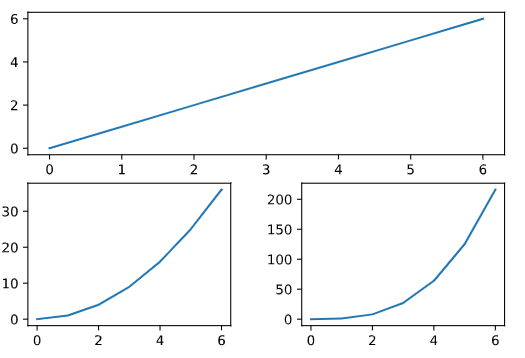
\includegraphics[scale=.55]{subadj}
	\end{minipage} \\
	We can add a \textbf{legend} to our graph, be either passing a list of strings to the .legend( ) method or passing the keywords label=`` " to the .plot method and then calling plt.legend( ) afterwards with no parameters.
	\begin{lstlisting}
	months = range(12)
	hyrule = [63, 65, 68, 70, 72, 72, 73, 74, 71, 70, 68, 64]
	kakariko = [52, 52, 53, 68, 73, 74, 74, 76, 71, 62, 58, 54]
	
	plt.plot(months, hyrule) # could also pass label="Hyrule"
	plt.plot(months, kakariko) # could also pass label="Kakariko"
	
	plt.legend(["Hyrule", "Kakariko"], loc=8) # default loc is 'best position'
	
	plt.show() \end{lstlisting}\vspace*{1mm}
	We can \textbf{modify tick marks} by creating an axes object and modifying the axes of that specific subplot.
	\begin{minipage}[c]{10cm}
	\begin{lstlisting}
	month_names = ["Jan", "Feb", "Mar", "Apr", 
	               "May", "Jun", "Jul", "Aug", 
	               "Sep","Oct", "Nov", "Dec"]
		
	months = range(12)
	conversion = [0.05, 0.08, 0.18, 0.28, 0.4, 0.66, 
		          0.74, 0.78, 0.8, 0.81, 0.85, 0.85]
		
	plt.xlabel("Months")
	plt.ylabel("Conversion")
		
	plt.plot(months, conversion)
		
	ax = plt.subplot() # create axes object
	ax.set_xticks(months) # set x ticks to months
	ax.set_xticklabels(month_names) # string labels
	ax.set_yticks([0.10, 0.25, 0.5, 0.75])
	ax.set_yticklabels(["10%", "25%", "50%", "75%"])
		
	plt.show() \end{lstlisting}\vspace*{1mm}
	\end{minipage}
	\begin{minipage}[c]{7cm}
		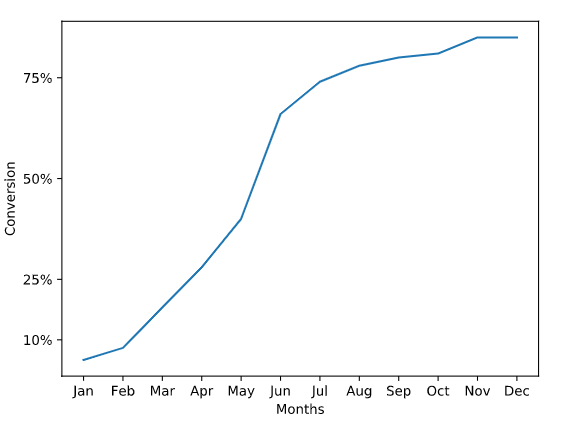
\includegraphics[scale=.52]{ticks}
	\end{minipage} \\
	We can create \textbf{figures} and save them to an output file on our system using the following commands.
	\begin{lstlisting}
	plt.close('all') # clear all existing plots before new one is plotted
	plt.figure(figsize=(7,3)) # creat a figure with width = 7in, height = 3in
	plt.plot(years, power_generated) # plot our data (instead of showing, save to file)
	plt.savefig('power_generated.png') # can also save as .pdf or .svg \end{lstlisting} \newpage
%%%% PAGE 54 %%%%

	\noindent LIME GRAPHING PROJECT
	\begin{lstlisting}
	months = ["Jan", "Feb", "Mar", "Apr", "May", "Jun", "Jul", "Aug", "Sep", "Oct", 
	"Nov", "Dec"]
	
	visits_per_month = [9695, 7909, 10831, 12942, 12495, 16794, 14161, 12762, 
	12777, 12439, 10309, 8724]
	
	# numbers of limes of different species sold each month
	key_limes_per_month = [92.0, 109.0, 124.0, 70.0, 101.0, 79.0, 106.0, 101.0, 
	                       103.0, 90.0, 102.0, 106.0]
	persian_limes_per_month = [67.0, 51.0, 57.0, 54.0, 83.0, 90.0, 52.0, 63.0, 
	                           51.0, 44.0, 64.0, 78.0]
	blood_limes_per_month = [75.0, 75.0, 76.0, 71.0, 74.0, 77.0, 69.0, 80.0, 
	                         63.0, 69.0, 73.0, 82.0]
	
	plt.figure(figsize=(12,8)) # create new figure
	ax1 = plt.subplot(1,2,1) # axes object for left plot
	x_values = range(len(months))
	plt.plot(x_values, visits_per_month, marker='o')
	plt.xlabel("Months")
	plt.ylabel("Number of Visits")
	ax1.set_xticks(x_values)
	ax1.set_xticklabels(months)
	plt.title("Number of Visits per Month")
	
	ax2 = plt.subplot(1,2,2) # axes object for right plot
	plt.plot(x_values, key_limes_per_month, color='green', label='Key Limes')
	plt.plot(x_values, persian_limes_per_month, color='orange', label='Persian Limes')
	plt.plot(x_values, blood_limes_per_month, color='red', label='Blood Limes')
	plt.legend()
	ax2.set_xticks(x_values)
	ax2.set_xticklabels(months)
	plt.title("Lime Sales by Type per Month")
	
	plt.subplots_adjust(wspace=0.3)
	plt.savefig("LimeGraphComparison.png")
	plt.show() \end{lstlisting}\vspace*{1mm}
	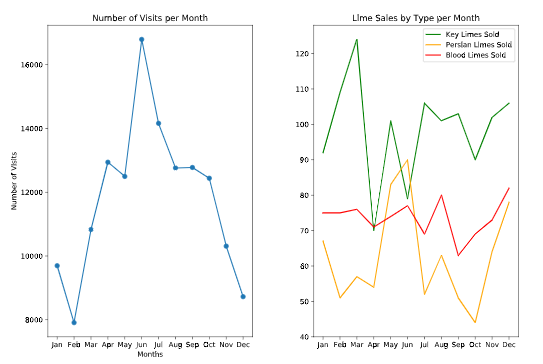
\includegraphics[scale=.95]{lime} \newpage
%%%% PAGE 55 %%%%
	
	\subsubsection{Different Plot Types \& Error}
	We can create \textbf{simple bar charts} to compare multiple categories of data with the plt.bar( ) function.\\
	\hspace*{3mm} - Note: We want our x to have the same number of elements as y, often we use range(len(y\_value))
	\begin{minipage}[c]{9cm}
	\begin{lstlisting}
	drinks = ["cappuccino", "latte", "chai", 
	          "americano", "mocha", "espresso"]
	sales =  [91, 76, 56, 66, 52, 27]
	# create bar graph
	plt.bar(range(len(drinks)), sales) 
	# create axes object
	ax = plt.subplot()
	ax.set_xticks(range(len(drinks)))
	# label each x to corresponding drinks
	ax.set_xticklabels(drinks, rotation=20)	
	plt.show() \end{lstlisting}\vspace*{1mm}
	\end{minipage}
	\begin{minipage}[c]{8cm}
		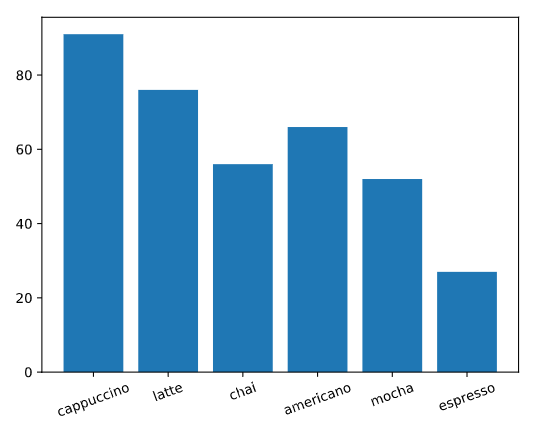
\includegraphics[scale=.5]{barchart}
	\end{minipage} \vspace*{1mm} \\
	We can use \textbf{side-by-side bar charts} to compare two sets of data with the same types of axis values. We must generate the x-axis values using list comprehension (same formula every time). \\
	\begin{minipage}[c]{9.2cm}
	\begin{lstlisting}
	drinks = ["cappuccino", "latte", "chai", 
	          "americano", "mocha", "espresso"]
	sales1 =  [91, 76, 56, 66, 52, 27]
	sales2 = [65, 82, 36, 68, 38, 40]
	
	n = 1  # Current dataset number
	t = 2 # Number of datasets
	d = 6 # Number of sets of bars
	w = 0.8 # Width of each bar
	store1_x = [t*element + w*n for element in 
	            range(d)]
	
	n=2 # 2nd dataset number (use prev. t,d,w)
	store2_x = [t*element + w*n for element in 
	            range(d)]
	
	plt.bar(store1_x, sales1) #plot first bar
	plt.bar(store2_x, sales2) # plot 2nd bar
	plt.show() # display graph \end{lstlisting}\vspace*{1mm}
	\end{minipage}
	\begin{minipage}[c]{8cm}
		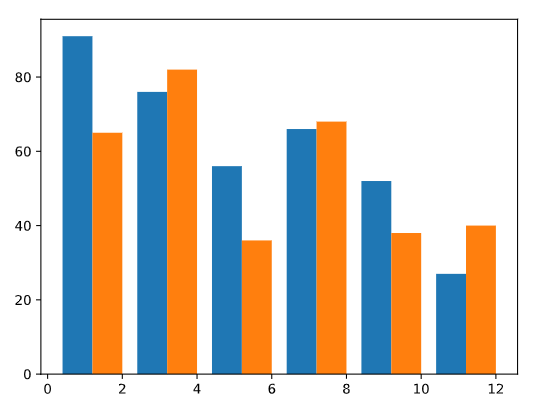
\includegraphics[scale=.57]{sidebyside}
	\end{minipage} \vspace*{1mm} \\
	We can use \textbf{stacked bar charts} to compare two data sets while preserving the total between them. We do this by plotting the first graph, then passing the keyword `bottom=' for the 2nd graph to be on top. \href{https://matplotlib.org/3.1.1/gallery/lines_bars_and_markers/bar_stacked.html}{Click here} for visual of graph style.
	\begin{lstlisting}
	# use datasets from above: drinks, sales1, sales2 
	
	plt.bar(range(len(drinks)), sales1, label='Location 1')
	plt.bar(range(len(drinks)), sales2, bottom=sales1, label='Location 2')
	plt.legend()
	plt.show() \end{lstlisting}\vspace*{1mm}
	We can visually represent uncertainty in our graph through using \textbf{error bars}, by passing the keywords `yerr' and `capsize' to the plt.bar( ) function. Note that you can change the error for each y-value by passing a list to yerr. (Click above link in stacked bar chart section to see example of yerr).
	\begin{lstlisting}
	drinks = ["cappuccino", "latte", "chai", "americano", "mocha", "espresso"]
	ounces_of_milk = [6, 9, 4, 0, 9, 0]
	error = [0.6, 0.9, 0.4, 0, 0.9, 0]
	
	plt.bar(range(len(drinks)), ounces_of_milk, yerr=error, capsize=5)
	plt.show() \end{lstlisting} \newpage
%%%% PAGE 56 %%%%
	
	\noindent Just like in bar charts, we can represent \textbf{error in line graphs} by using the .fill\_between( ) method and passing x-values, lower y bounds, upper y bounds, and alpha. We also must use list comprehension to calculate the upper/lower y bounds from the original y-values. (note: alpha changes error transparency).\\
	\begin{minipage}[c]{9.2cm}
	\begin{lstlisting}
	months = range(12)
	month_names = ["Jan", "Feb", "Mar", "Apr", 
	               "May", "Jun", "Jul", "Aug", 
	               "Sep", "Oct", "Nov", "Dec"]
	revenue = [16000, 14000, 17500, 19500, 
	           21500, 21500, 22000, 23000, 
 	           20000, 19500, 18000, 16500]
	
	y_lower = [0.9*i for i in revenue]
	y_upper = [1.1*i for i in revenue]
	
	ax = plt.subplot()
	plt.fill_between(months, y_lower, y_upper, 
	                 alpha=0.2)
	plt.plot(months, revenue, marker=".")
	ax.set_xticks(months)
	ax.set_xticklabels(month_names)
	plt.show() \end{lstlisting}\vspace*{1mm}
	\end{minipage}
	\begin{minipage}[c]{8cm}
		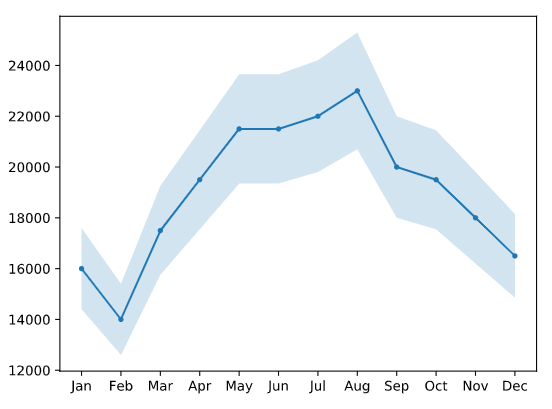
\includegraphics[scale=.57]{lineerr}
	\end{minipage} \vspace*{1mm} \\
	We can use \textbf{pie charts} to display elements of a data set as proportions of a whole by using plt.pie( ). Note that it will be tilted and we don't want this, so we must past plt.axis(``equal'') to flatten. Labeling a pie chart can be done in two different ways: \\ 
	\hspace*{3mm} - Use plt.legend( ) to create a color coded legend for each slice \\
	\hspace*{3mm} - Pass the keyword \textit{labels=` '} to plt.pie( ) to add labels on each slice \\
	We can also add the percent to the pie chart by passing the keyword autopct=` ' to the plt.pie( ) function
	\begin{lstlisting}
	payment_method_names = ["Card Swipe", "Cash", "Apple Pay", "Other"]
	payment_method_freqs = [270, 77, 32, 11]
	
	plt.pie(payment_method_freqs, autopct='%0.1f%%') # to 1 decimal place with % sign
	plt.axis('equal') # flatten our pie chart
	plt.legend(payment_method_names) # create color coded legend for graph
	plt.show() \end{lstlisting}\vspace*{1mm}
	We can create \textbf{histograms} to find a more intuitive sense for a dataset and see how many values fall in between a certain range. We do this by calling plt.hist( ). Note that we can also compare two different distribution by plotting multiple histograms, but we need to know a few keywords for this: \\
	\hspace*{3mm} - \textit{bins=} changes the number of bins to divide the data into (default is 10) \\
	\hspace*{3mm} - \textit{range=( )} to change the x-axis display value range \\
	\hspace*{3mm} - \textit{alpha=} to change the transparency of our graphs (lets us see overlap of 2 histograms) \\
	\hspace*{3mm} - \textit{histtype=`step'} will only draw the outline of our graphs (good for viewing overlap) \\
	\hspace*{3mm} - \textit{normed=True} will normalize the data so total shaded area = 1 (good for different sized data sets)
	\begin{minipage}[c]{9cm}
	\begin{lstlisting}
	# plot the first histogram (blue)
	plt.hist(sales_times1, bins=20, alpha=0.4, 
	         normed=True)
	
	# plot the second histogram (orange)
	plt.hist(sales_times2, bins=20, alpha=0.4, 
	         normed=True)
	
	plt.show() # overlap is brown \end{lstlisting}\vspace*{1mm}
	\end{minipage}
	\begin{minipage}[c]{9cm}
		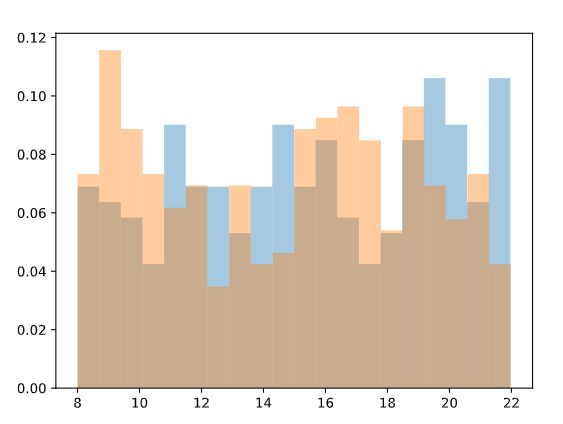
\includegraphics[scale=.48]{multhist}
	\end{minipage} \newpage
%%%% PAGE 57 %%%%
	
	\subsubsection{Selecting the Correct Visualization}
	The three steps of the data visualization process are \textit{preparing, visualizing, and styling}. We often wonder which chart to use (the visualization stage), so we can use this diagram to help us select a chart based on the data we are using and the question we are focusing on: \\~\\
	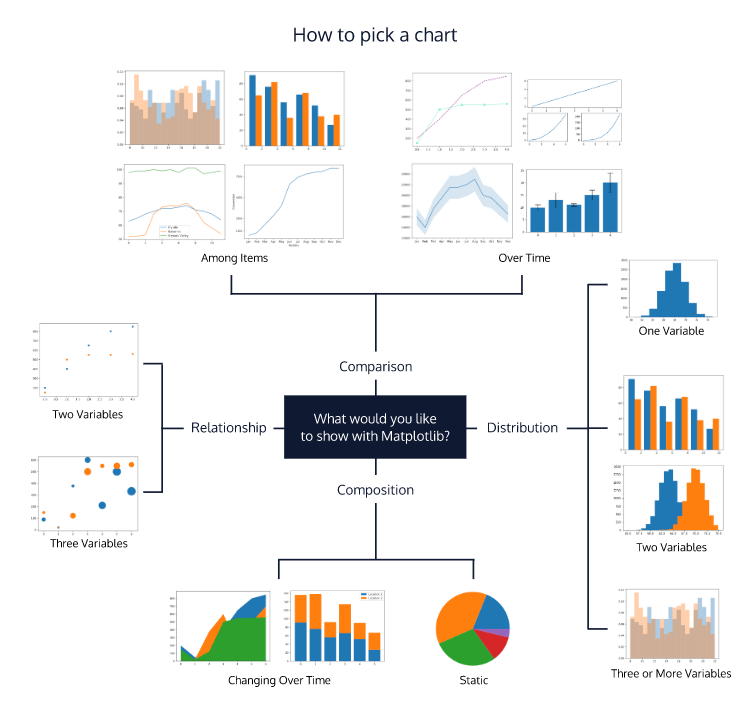
\includegraphics[scale=.8]{visdiag} \\
	\textbf{Composition Charts} - Used when asking ``what are the parts of some whole" or ``what is the data made of". Data pertaining to proportions or percentages as a whole are a good fit. \vspace*{2mm} \\
	\textbf{Distribution Charts} - Data in large quantities work well (see patterns, re-occurrences, clustering). Data that we want to see its ``distribution'' of is a good fit (such as seeing a normal dist. in statistics). \vspace*{2mm} \\
	\textbf{Relationship Charts} - Used when asking ``how do variables relate to each other". Data with two or more variables area good fit (used to see correlation between them). \vspace*{2mm} \\
	\textbf{Comparison Charts} - Used when asking ``how do variables compare to each other". Data must have multiple variables and are being used to compare against one another. \\~\\
	\textbf{Resources}: \\
	1) \href{https://s3.amazonaws.com/codecademy-content/courses/matplotlib/data_vis_matplotlib_cheatsheet_v1_revisons.pdf}{Matplotlib Cheat Sheet} from Codecademy. \\
	2) \href{https://matplotlib.org/tutorials/index.html}{Tutorials from Matplotlib website}. \\
	3) See `Constellation` project in Python folder for \underline{scatter plot} and \underline{3d rotations} in Matplotlib. \newpage
%%%% PAGE 58 %%%%

	\subsection{Introduction to Seaborn}
	Seaborn is a Python data visualization library that provides simple code to create elegant visualizations for statistical exploration and insight. Seaborn is based on Matplotlib, but improves on Matplotlib in several ways: \\	
	\hspace*{3mm} - Seaborn provides a more visually appealing plotting style and concise syntax. \\
	\hspace*{3mm} - Seaborn natively understands Pandas DataFrames, making it easier to plot data directly from CSVs. \\
	\hspace*{3mm} - Seaborn can easily summarize Pandas DataFrames with many rows of data into aggregated charts. \vspace*{2mm}\\
	Assume the following imports are all done in the examples:
	\begin{lstlisting}
	import pandas as pd
	from matplotlib import pyplot as plt
	import seaborn as sns
	import numpy at np \end{lstlisting}\vspace*{1mm}
	Seaborn has a much simpler way to create \textbf{bar charts} compared to Matplotlib, and we can do so with the function sns.barplot( ) and the following three keywords: \\
	\hspace*{3mm} - \textit{data=} is a Pandas DataFrame that contains the data. \\
	\hspace*{3mm} - \textit{x=} is a string that tells Seaborn which column in the DataFrame contains x-labels. \\
	\hspace*{3mm} - \textit{y=} is a string that tells Seaborn which column in the DataFrame contains y-values. \\ 
	Note: By default, Seaborn will aggregate and plot the mean of each category. 
	\begin{lstlisting}
	df = pd.read_csv('results.csv') # contains columns 'Gender' and 'Mean Satisfaction'
	sns.barplot(x='Gender', y='Mean Satisfaction', data= df)
	plt.show()\end{lstlisting}\vspace*{1mm}
	Seaborn can also calculate \textbf{aggregate statistics} (a single number used to describe a set of data) for large datasets. We can use NumPy to calculate these aggregates from our DataFrames. 
	\begin{lstlisting}
	gradebook = pd.read_csv("gradebook.csv")
	
	assignment1 = gradebook[gradebook.assignment_name == 'Assignment 1']
	asn1_median = np.median(assignment1.grade)	
	
	# Seaborn will agregate grade by assignment_name and plot average grade for both 
	# assignment 1 and assignment 2
	sns.barplot(data=gradebook, x='assignment_name', y='grade')
	plt.show()\end{lstlisting}\vspace*{1mm}
	By default, the barplot( ) function will place \textbf{error bars} (the range of values that might be expected for that bar) on all of our bars in the graph. By default, Seaborn uses a \textit{bootstrapped confidence interval} at a 95\% confidence level (but we can change the error types of these bars using the \textit{ci=} keyword). 
	\begin{lstlisting}
	gradebook = pd.read_csv("gradebook.csv")
	
	# change error bars to one standard deviation instead of 95% confidence intervals
	sns.barplot(data=gradebook, x="name", y="grade", ci='sd')\end{lstlisting}\vspace*{1mm}
	We can \textbf{calculate different aggregates} than just the mean of our data (Seaborn's default aggregate) by using the \textit{estimator=} keyword, which accepts any function that works on a list. Some examples: \\
	\hspace*{3mm} - np.median : use if our data has many outliers. \\
	\hspace*{3mm} - len : how many times a value appears (categorical data). 
	\begin{lstlisting}
	df = pd.read_csv("survey.csv")
	
	# Show how many men and women answered the survey (grouped by gender)
	sns.barplot(data=df, x='Gender', y='Response', estimator=len)
	# Show the median response value aggregated by gender
	sns.barplot(data=df, x='Gender', y='Response', estimator=np.median)\end{lstlisting}\newpage
%%%% PAGE 59 %%%%
	
	\noindent We can \textbf{aggregate by multiple columns} to visualize nested categorical variables. We can compare two columns at once by using the keyword \textit{hue=} to add a nested categorical variable to the plot.
	\begin{minipage}[c]{9cm}
	\begin{lstlisting}
	gradebook = pd.read_csv("gradebook.csv")
	
	# Visualize mean response value by gender 
	# with age range nested
	sns.barplot(data=df, x="Gender", 
 	            y="Response", 
	            hue="Age Range")
	plt.show() \end{lstlisting}\vspace*{1mm}
	\end{minipage}
	\begin{minipage}[c]{10cm}
		\hspace*{5mm} 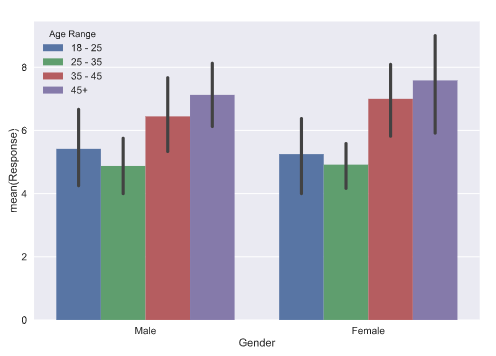
\includegraphics[scale=.5]{seamult}
	\end{minipage} \\
	\subsubsection{Plotting Distributions}
	One of the most powerful aspects of Seaborn is its ability to visualize and compare distributions. Calculating and graphing distributions is integral to analyzing massive amounts of data. We’ll look at how Seaborn allows us to communicate important statistical information through plots. \vspace*{2mm} \\
	We can use \textbf{KDE Plots} (Kernel Density Estimator) to give us the sense of a univariate (only on varaible, `one-dimensional') as a curve. KDE plots are preferable to histograms because they smooth the datasets and allow us to generalize over the shape of our data (and aren't beholden to specific data points).
	\begin{minipage}[c]{10.3cm}
	\begin{lstlisting}
	# Take in the data from the CSVs as NumPy arrays:
	s1 = np.genfromtxt("dataset1.csv", delimiter=",")
	s2 = np.genfromtxt("dataset2.csv", delimiter=",")
	s3 = np.genfromtxt("dataset3.csv", delimiter=",")
	s4 = np.genfromtxt("dataset4.csv", delimiter=",")
	
	sns.set_style("darkgrid") # set style
	
	# Plot the 4 datasets
	sns.kdeplot(s1, shade=True) 
	sns.kdeplot(s2, shade=True) # bimodal (two peaks)
	sns.kdeplot(s3, shade=True) # skewed left
	sns.kdeplot(s4, shade=True) # normal-ish
	plt.legend(['set 1', 'set 2', 'set 3', 'set 4'])
	plt.show() \end{lstlisting}\vspace*{1mm}
	\end{minipage}
	\begin{minipage}[c]{10cm}
		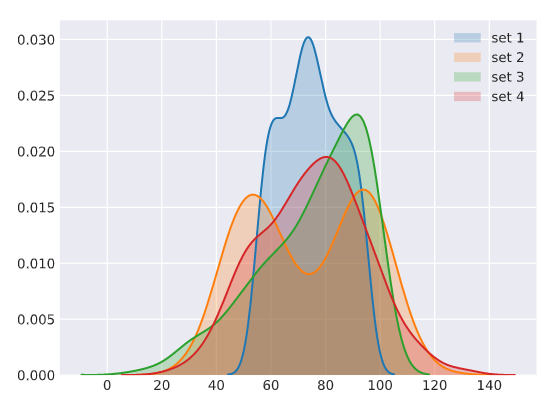
\includegraphics[scale=.48]{kde}
	\end{minipage} \\
	We can use \textbf{box plots} to show us the range of our dataset, give us an idea about where a significant portion of our data lies, and whether or not any outliers are present. We interpret a box plot as: the \textit{box} represents interquartile range, the \textit{line in the middle} of the box is the mean, the \textit{end lines} are the first and third quartiles, and the \textit{diamonds} show outliers. \\
	\hspace*{3mm} - An advantage of box plots over KDE is that it's easy to plot multiples and compare range of values. \\
	\hspace*{3mm} - Note that it shows the range of values and not the curve (distribution) of the datasets. \\
	\begin{minipage}[c]{10.3cm}
	\begin{lstlisting}
	n=500
	df = pd.DataFrame({ # using s1-s4 from above
		"label": ["set_one"] * n + ["set_two"] * n + 
		         ["set_three"] * n + ["set_four"] * n,
		"value": np.concatenate([s1, s2, s3, s4])
	})
	
	sns.set_style("darkgrid") # set style
	
	# Plot the 4 datasets using the dataframe
	sns.boxplot(data=df, x='label', y='value')
	plt.show()	\end{lstlisting}\vspace*{1mm}
	\end{minipage}
	\begin{minipage}[c]{10cm}
		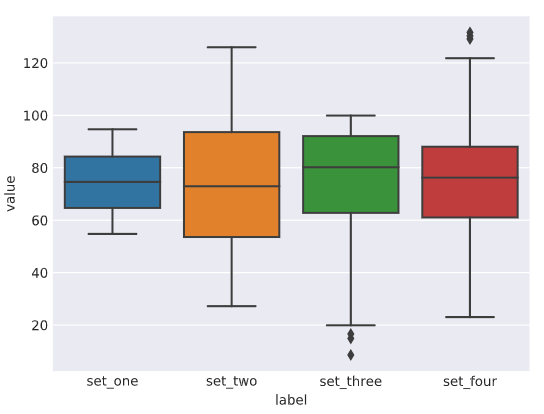
\includegraphics[scale=.48]{bpdist}
	\end{minipage} \newpage
%%%% PAGE 60 %%%%
	
	\noindent We can use \textbf{violin plots} to compare distributions by giving us an estimation of the dataset. It can show us the distribution (like the KDE plot) and information about the median/interquartile range (like the box plot). They are trickier to read and can be broken down to the following parts: \\
	\hspace*{3mm} - There are two \textit{KDE plots} that are symmetrical along the center line. \\
	\hspace*{3mm} - A \textit{white dot} represents the median. \\
	\hspace*{3mm} - The \textit{thick black line} in the center of each violin represents the interquartile range. \\
	\hspace*{3mm} - The \textit{lines extending from the center} are 95\% confidence intervals for our data. \\
	\begin{minipage}[c]{10.3cm}
	\begin{lstlisting}
	# using s1, s2, s3, and s4 from above
	# and using df from above
	
	sns.set_style("darkgrid") # set style
	
	# plot the 4 distributions using violin plot
	sns.violinplot(data=df, x='label', y='value')
	plt.show()
	# notice we see the same distributions from KDE
	# and same ranges from the boxplot \end{lstlisting}\vspace*{1mm}
	\end{minipage}
	\begin{minipage}[c]{10cm}
		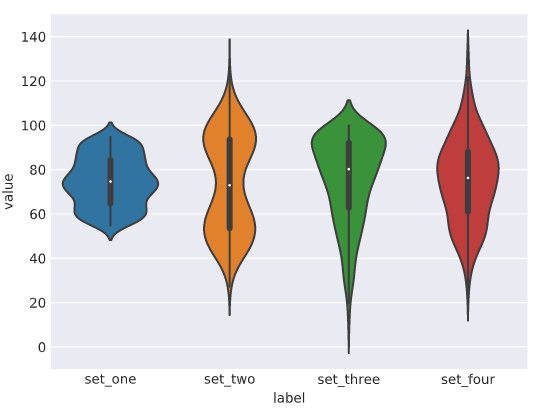
\includegraphics[scale=.48]{violin}
	\end{minipage} \\
	
	\subsubsection{Styling Graphs}
	Styling your graphs will influence how your audience understands what you're trying to convey. When deciding the style, ask yourself: is it part of a report, is it part of a presentation, is it stand alone with no explanation? These questions will help decide which style to chose in order to best convey your data. \\~\\
	Seaborn has five \textbf{built in themes}: darkgrid, whitegrid, dark, white, and ticks. All of which can be passed into the sns.set\_style( ) method. \vspace*{2mm} \\
	It is important to consider \textbf{background color}. The higher the contrast between you plot color palette and the figure background, the more legible the data visualization will be. \vspace*{2mm} \\
	Including a \textbf{grid} can be helpful when you want your audience to be able to draw their own conclusions about data. Research papers and reports are a good example of when you would want to include a grid.\vspace*{2mm} \\
	We can remove \textbf{spines} from plots (the four black borders that contain the graph) by using sns.despine(), which by default will remove the top/right spines (can pass \textit{left=True, bottom=True} to remove all spines).\vspace*{2mm} \\
	We can \textbf{customize plots for presentation} by using sns.set\_context( ) and passing these keywords: \\
	\hspace*{3mm} - the first parameter adjusts the scale of the plot: `paper', `notebook', `talk', `poster'. \\
	\hspace*{3mm} - \textit{font\_scale=} will change the size of the text. \\
	\hspace*{3mm} - \textit{rc=} will let us change any value in a dictionary (run sns.plotting\_context() to see which values can 
	\hspace*{5.5mm} be changed). \vspace*{2mm} \\
	We can change \textbf{palette color} with two different functions, sns.color\_palette( ) and sns.set\_pallete( ). \\
	\hspace*{3mm} - sns.color\_palette( ) can be saved to a variable, then passed in sns.palplot( ) to see an array of colors. \\
	\hspace*{3mm} - sns.set\_pallete( ) is passed the name of the pallete you want to use for the plot. \vspace*{2mm} \\
	Note: you can also use \href{https://colorbrewer2.org/#type=sequential&scheme=BuGn&n=3}{Color Brewer Palettes} instead of the default Seaborn colors by passing the name and number of colors needed.
	\begin{lstlisting}
	palette = sns.color_palette("bright") # to visualize the colors in a pallete
	sns.palplot(palette) 
	
	sns.set_palette("Paired") # to set the pallete for the plot
	sns.set_palette("Set3", 10) # color brewer pallete with 10 different shades	\end{lstlisting} \vspace*{1mm}
	See `Kiva Loans (Seaborn Project)' in \textit{DS Projects} folder for final Seaborn project.\newpage
%%%% PAGE 61 %%%%

	\subsection{Data Visualization Cumulative Project (Matplotlib)}
	\begin{lstlisting}
	restaurants = pd.read_csv('restaurants.csv')
	orders = pd.read_csv('orders.csv')
	
	##### Q1: What cuisines does FoodWheel offer? What area should they focus on? #####
	
	# count number of different types of cuisines offered (returns int)
	cuisine_options_count = restaurants.cuisine.nunique()
	
	# number of restaurants for each cuisine offered (returns table)
	cuisine_counts = restaurants.groupby('cuisine').name.count().reset_index()
	
	cuisines = cuisine_counts.cuisine.values # list of cuisine names
	counts = cuisine_counts.name.values # number of restaruants of each cuisine
	
	# plot a pie chart of number of restuarants offereing certain cuisines 
	plt.pie(counts, autopct='%d%%', labels=cuisines)
	plt.title('Number of Restaurants Offering Cuisine Types')
	plt.axis('equal')
	plt.show() # see (Figure 1) below
	
	############### Q2: How has average order amount changed over time? ###############
	
	# create new column with month (extract from date column)
	orders['month'] = orders.date.apply(lambda x: x.split('-')[0])
	
	avg_order = orders.groupby('month').price.mean().reset_index() # avg order price
	std_order = orders.groupby('month').price.std().reset_index() # std of order price
	
	bar_heights = avg_order.price.values # average order prices
	bar_errors = std_order.price.values # standard dev of prices
	
	ax = plt.subplot()
	plt.bar(range(len(bar_heights)), bar_heights, yerr=bar_errors, capsize=5)
	plt.ylabel('Average Order Price')
	plt.title('Average Order Price by Month (Figure 2)')
	ax.set_xticks(range(len(avg_order)))
	ax.set_xticklabels(['April', 'May', 'June', 'July', 'August', 'September'])
	plt.show() # see (Figure 2) below
	
	### Q3: How much has each customer on FoodWheel spent over the past six months? ###
	
	c_amount = orders.groupby('customer_id').price.sum().reset_index() # total each cust
	
	plt.hist(c_amount.price.values, range=(0, 200), bins=40)
	plt.xlabel('Total Spent')
	plt.ylabel("Number of Customers")
	plt.title('Customer Expenditure Over 6 Months (Figure 3)')
	plt.show() # see (Figure 3) below	\end{lstlisting}\vspace*{1mm}
	\begin{minipage}[c]{5.5cm}
		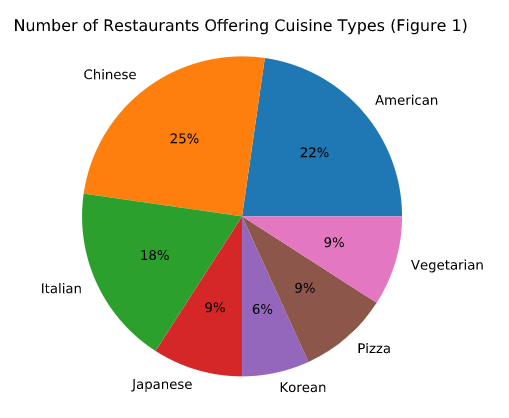
\includegraphics[scale=.39]{figure1}
	\end{minipage}
	\begin{minipage}[c]{6cm}
		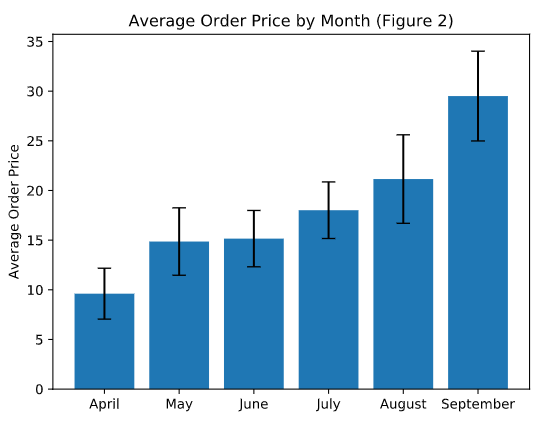
\includegraphics[scale=.39]{figure2}
	\end{minipage}
	\begin{minipage}[c]{6cm}
		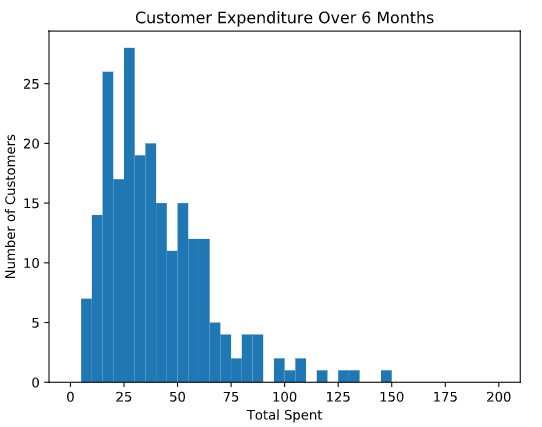
\includegraphics[scale=.39]{figure3}
	\end{minipage} \newpage
%%%% PAGE 62 %%%%
	
	\section{Statistics in Python}
	\subsection{Basic Statistical Calculations}
	We can us the \textbf{NumPy} and \textbf{SciPy} library to find statistical values from CSV's and NumPy arrays. \\
	\hspace*{3mm} - \textbf{mean}: the average value in a list of numbers (sum / number of elements). \\
	\hspace*{3mm} - \textbf{median}: the value that falls in the middle of a sorted dataset (smallest to largest). \\
	\hspace*{8mm} - note: the np.median( ) function will automatically sort the list for you. \\
	\hspace*{3mm} - \textbf{mode}: the most frequently occurring observation in a dataset (can have multiple).\\
	\hspace*{8mm} - note: this will return an object, access mode by var\_name[0][0], frequency by var\_name[1][0]. \\
	\hspace*{8mm} - note 2: if there are two modes, stats.mode( ) will return the smallest value only.
	\begin{lstlisting}
	from scipy import stats
	import numpy as np
	
	greatest_books = pd.read_csv("top-hundred-books.csv")
	author_ages = greatest_books['Ages']
	
	average_age = np.average(author_ages) # mean (42.12)
	median_age = np.median(author_ages) # median (41.0)
	mode_age = stats.mode(author_ages) # mode (38, frequency = 7) \end{lstlisting}\vspace*{1mm}
	\textbf{Variance} ($\sigma^2$) is a descriptive statistic that describes how spread out the points in a data set are. We get this by taking the squared difference of the data points from the mean (X - $\mu$)$^2$, adding them all up, and then finding the average. (note that variance in measured in \textit{units squared}).
	\begin{lstlisting}
	#using the dataframe from above and the author_ages list
	var_age = np.var(author_ages) \end{lstlisting}\vspace*{1mm}
	\textbf{Standard deviation} ($\sigma$) is computed by taking the square root of the variance and is measured in the correct units (easily interpreted and compared to mean). We can expect 68\% of the data to fall within 1 std of the mean, 95\% to fall within 2 std's of the mean, and 99.7\% to fall within 3 std's of the mean.
	\begin{lstlisting}
	#using the dataframe from above and the author_ages list
	var_age = np.std(author_ages) \end{lstlisting}\vspace*{4mm}
	
	\subsection{Histograms}
	A \textbf{histogram} displays the distribution of your underlying data, and reveals interpretable trends. Two keys features of histograms are \textit{bins} and \textit{counts}. \\
	\hspace*{3mm} - bin: a sub-range of value that falls within the range of a dataset (must all be same width). \\
	\hspace*{3mm} - count: the number of values that fall within a bin's range.	\\
	\hspace*{3mm} - np.histogram( ) takes an array, range, and bin count to calculate the frequency for each range. \\
	\hspace*{7mm} - note: the first array returned is the y value, the second is the range up to the following number.
	\begin{lstlisting}
	transactions = pd.read_csv("transactions.csv")
	times = transactions["Transaction Time"].values # create numpy array
	cost = transactions["Cost"].values # create numpy array
	
	# find the range of the times 
	min_time = np.amin(times) # 0.02661518360957871
	max_time = np.amax(times) # 23.675374635328755
	range_time = max_time - min_time # 23.648759451719176
	
	times_hist = np.histogram(times, range=(0,24), bins=4)
	# (array([101, 231, 213, 455]), array([ 0.,  6., 12., 18., 24.])) 
	# example interpetation: range 0-5.9 has 101 values, 6-11.9 has 231 values \end{lstlisting} \newpage
%%%% PAGE 63 %%%%

	\noindent Histograms are typically viewed \textbf{graphically}, and it becomes harder to interpret the np.histogram( ) function as our number of bins increase. By using plt.hist( ) from matplotlib and the same parameters as np.histogram( ) we can create a visual to see and trends in our data. 
	\begin{lstlisting}[language=Python]
	# using times list from above
	plt.hist(times, range=(0,24), bins=4) # this will graphiclly display times_hist above\end{lstlisting}\vspace*{1mm}
	When plotting a histogram, it’s essential to \textbf{select bins that fully capture the trends} in the underlying data. Often, this will require some guessing and checking. By changing the number of bins in our example above from 4 to 24, we can see that instead of the highest frequency being 18-24 (with 4 bins), the highest values are now from 17-22 (with 24 bins). \\~\\
	Now that we can plot and find values of a histogram, we will learn \textbf{how to describe a histogram} to communicate the correct information. We will take a look at five features of a dataset. \\
	\hspace*{3mm} - center: we will use average and median as our measure of centrality. \\
	\hspace*{3mm} - spread: we will us the minimum, maximum, and range as our measure. \\
	\hspace*{3mm} - skew: the symmetry of our data (can be symmetric, right-skew, or left-skew). \\
	\hspace*{3mm} - modality: the number of peaks in a dataset (uniform(0), unimodal(1), bimodal(2), multimodal(2+)). \\
	\hspace*{3mm} - outliers: a point far away from the rest of the data (report and investigate). \vspace*{1mm} \\
	\begin{minipage}[c]{8cm}
		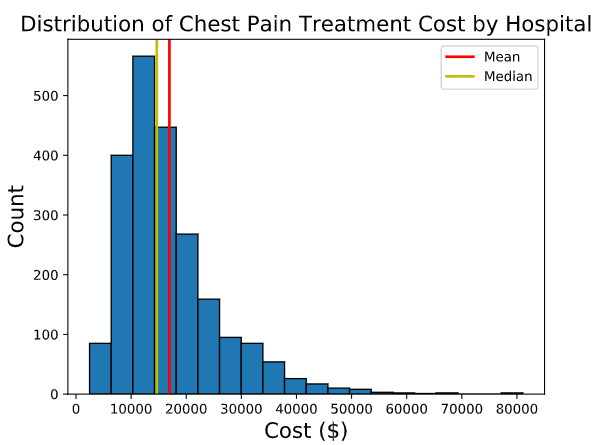
\includegraphics[scale=.5]{chest}
	\end{minipage}
	\begin{minipage}[c]{9.5cm}
		This histogram displays the distribution of chest pain cost for over 2,000 hospitals across the United States. The average and median costs are \textit{\$16,948} and \textit{\$14,659.6}, respectively. Given that the data is \textit{unimodal}, with one local maximum and a \textit{right skew}, the fact that the average is \textit{greater} than the median, matches our expectation. The range of costs is very large, \textit{\$78,623}, with the smallest cost equal to \textit{\$2,459} and the largest cost equal to \textit{\$81,083}. There is one hospital, \textit{Bayonne Hospital Center}, that charges far more than the rest at \textit{\$81,083}.
	\end{minipage} \vspace*{4mm}
	
	\subsection{Quartiles, Quantiles, and Interquartile Range}
	A common way to communicate a high-level overview of a dataset is to find the values that split the data into four groups of equal size, called \textbf{quartiles} (split into Q1, Q2, Q3, Q4). \\
	\hspace*{3mm} - Q2: this is the middle value (to find it, sort the list and take the median of it). \\
	\hspace*{3mm} - Q1: this is the middle of all the values below Q2 (between minimum and median). \\
	\hspace*{3mm} - Q3: this is the middle of all the value above Q3 (between median and max). \\
	\hspace*{3mm} - note: when calculating Q1 and Q3, you can include or exclude the median from the calculation. \vspace*{2mm} \\
	We can use \textbf{NumPy to find quartiles} by using the \textit{np.quantile( )} function (a quartile is just a specific quantile). We pass two parameters to it, the dataset and a number between 0-1 (quartile percent). 
	\begin{lstlisting}
	from song_data import songs
	import numpy as np
	
	songs_q1 = np.quantile(songs, 0.25) # Q1 (25%)
	songs_q2 = np.quantile(songs, 0.5) # Q2 (50%)
	songs_q3 = np.quantile(songs, 0.75) # Q3 (75%)	\end{lstlisting}\vspace*{1mm}
	Quartiles are so commonly used that the three quartiles, along with the minimum and maximum values of a dataset, are called the \textbf{five-number summary of the dataset}. These help you quickly get a sense of the range, centrality, and spread of the dataset. \newpage
%%%% PAGE 64 %%%%
	
	\noindent \textbf{Quantiles} are similar to quartiles, but can be expressed as any number (not just split into four). If you have \textit{n} quantiles, it will split the data into \textit{n+1} groups of equal size. Similar to above, we will use NumPy's \textit{np.quantile( )} function to separate the data. To evenly separate the data into multiple quantiles, we pass a list as our parameter. 
	\begin{lstlisting}
	quartiles = np.quantile(songs, [0.25, 0.5, 0.75]) # create quartiles (split into 4)
	deciles = np.quantile(songs, [i/10 for i in range(1,10)]) 
	# list comprehension to find quantile for every 10% (split into 10) \end{lstlisting}\vspace*{1mm}
	Common quantiles: \\
	\hspace*{3mm} - 2-quantile: splits the data in two groups of equal size (also known as the median). \\
	\hspace*{3mm} - 4-quantiles: split the data into four groups of equal size (also known as quartiles). \\
	\hspace*{3mm} - percentiles: split the data into 100 groups (used to compare new data points to dataset). \\~\\
	The \textbf{interquartile range (IQR)} is a descriptive statistic that tries to solve the problem of outliers affecting our range of a dataset. The IQR ignores the tails of the dataset, so you know the range around-which your data is centered. The IQR is the difference between Q3 and Q1 (the middle 50\%). \vspace*{1mm} \\
	We can calculate IQR by hand using NumPy, or find \textbf{IQR in SciPy} by using the \textit{iqr( )} function. Note that IQR is robust, meaning outliers have little impact on it, so two datasets IQR can be identical even with different outliers.
	\begin{lstlisting}
	from scipy.stats import iqr
	
	q1 = np.quantile(songs, 0.25) # calculate Q1
	q3 = np.quantile(songs, 0.75) # calculate Q3
	interquartile_range = q3 - q1 # 99.53959000000003
	
	interquartile_range = iqr(songs) # 99.53959000000003 \end{lstlisting}\vspace*{4mm}
	\textbf{Boxplots} are one of the most common ways to visualize a dataset, they give you a sense of the central tendency and spread of the data. Some of the key features of a boxplot are: \\
	\hspace*{3mm} - median: this is the line within the box (half the data above, half below). \\
	\hspace*{3mm} - interquartile range: these are the edges of the box (data between Q1 and Q3). \\
	\hspace*{3mm} - whiskers: these tell us about the spread of the data (usually 1.5 times the IQR, extend to the \hspace*{24mm} min/max values, or one standard deviation away from the box). \\
	\hspace*{3mm} - outliers: points that fall outside the whiskers (represented with a dot or asterisk). \vspace*{1mm} \\
	We can use \textbf{Matplotlib to make boxplots} by passing it a list (or multiple lists). 
	\begin{lstlisting}
	from music_data import two_thousand, two_thousand_one, two_thousand_two
	import matplotlib.pyplot as plt
	
	# create 3 boxplots on one graph
	plt.boxplot([two_thousand, two_thousand_one, two_thousand_two], 
	            labels = ["2000 Songs", "2001 Songs", "2002 Songs"]) \end{lstlisting}\vspace*{1mm}
	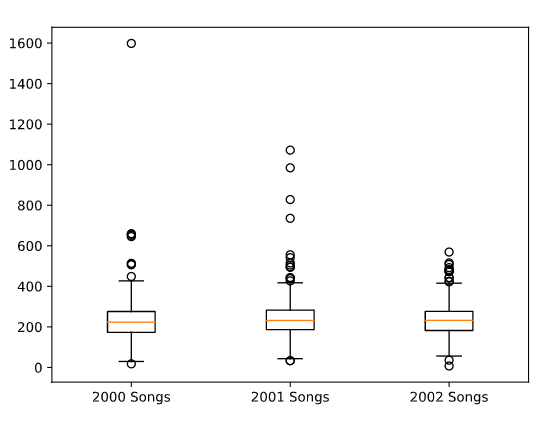
\includegraphics[scale=.4]{bpquart} \newpage
%%%% PAGE 65 %%%%

	\subsection{Introduction to NumPy}
	NumPy includes a powerful data structure known as an \textbf{array}. A NumPy array is a special type of list, and each item can be of any type (strings, numbers, or even other arrays). Note that we can also \textbf{transform a CSV into a NumPy array} using the \textit{np.genfromtxt( )} function. \\
	\hspace*{3mm} - note: the delimiter is how the data is separated in the CSV (could be a tab, colon, comma, etc.).
	\begin{lstlisting}
	import numpy as np
	
	test_1 = np.array([92, 94, 88, 91, 87])
	test_2 = np.genfromtxt('test_2.csv', delimiter=',') \end{lstlisting}\vspace*{1mm}
	Generally, NumPy arrays are more efficient than lists, they allow you to do \textbf{element-wise operations}. These can include addition, subtraction, power, etc on every element in a NumPy array (plus we can add/subtract multiple arrays). 
	\begin{lstlisting}
	test_1 = np.array([92, 94, 88, 91, 87])
	test_2 = np.array([79, 100, 86, 93, 91])
	test_3 = np.array([87, 85, 72, 90, 92])
	test_3_fixed = test_3 + 2 # add 2 to all array elements
	total_grade = test_1 + test_2 + test_3_fixed # add together all 3 arrays
	final_grade = total_grade / 3 # divide each element by 3
	print(final_grade) # [86 93 82 92 90] \end{lstlisting}\vspace*{1mm}
	We can create \textbf{two dimensional arrays} in NumPy (an array of arrays). Note that all arrays must have the same number of elements in order to create a two dimensional array. In statistics, we often use these to represent a set of samples (such as flipping a coin). \\
	\hspace*{3mm} - selecting elements: the syntax is array[row, column]. \\
	\hspace*{3mm} - there are two axes: axis 0 are elements in the same column, axis 1 are elements in the same row.
	\begin{lstlisting}
	student_scores = np.array([[92, 94, 88, 91, 87],
	                           [79, 100, 86, 93, 91],
	                           [87, 85, 72, 90, 92]])
	tanya_test_3 = student_scores [2,0] # 87
	cody_test_scores = student_scores[:,4] # [87 91 92] (all rows, last column) \end{lstlisting}\vspace*{1mm}
	Another useful thing that arrays can do is perform \textbf{element-wise logical operations}, which will return either T/F and can be used to create sub-arrays. 
	\begin{lstlisting}
	porridge = np.array([79, 65, 50, 63, 56, 90, 85, 98, 79, 51])
	
	cold = porridge[porridge < 60] # [50 56 51]
	hot = porridge[porridge > 80] # [90 85 98]
	just_right = porridge[(porridge > 60) & (porridge < 80)] # [79 65 63 79] \end{lstlisting}\vspace*{4mm}
	
	\subsubsection{Statistics with NumPy}
	We can use NumPy's built in function \textit{np.mean( )} to calculate the \textbf{mean} of our arrays (both 1-D and 2-D). We can also use \textbf{logical operators} to find the percent of an array that meets a given condition.
	\begin{lstlisting}
	allergy_trials = np.array([[6, 1, 3, 8, 2], 
	                           [2, 6, 3, 9, 8], 
	                           [5, 2, 6, 9, 9]])
	total_mean = np.mean(allergy_trials) # total of all elements
	trial_mean = np.mean(allergy_trials, axis=1) # for each row
	patient_mean = np.mean(allergy_trials, axis=0) # for each column
	
	print(total_mean) # 5.26666666667
	print(trial_mean) # [ 4.   5.6  6.2]
	print(patient_mean)	# [ 4.33333333  3.     4.     8.66666667  6.33333333] \end{lstlisting} \newpage
%%%% PAGE 66 %%%%
	
	\noindent \textbf{Outliers} (values that don’t fit within the majority of a dataset) can be used to determine if they were due to an error in sample collection or whether or not they represent a significant but real deviation from the mean. We can use \textit{np.sort( )} to sort our arrays and look at the end points to determine any outliers. \\~\\
	We can calculate the \textbf{median} of our dataset by using the \textit{np.median( )} function. \\~\\
	We can calculate \textbf{percentiles}, where the Nth percentile is defined as the point N\% of samples lie below it. These are useful measurements because they can tell us where a particular value is situated within the greater dataset. To do this, we can use the \textit{np.percentile( )} function. \\
	\hspace*{3mm} - \textit{Five-number summary}: minimum, first quartile, median, third quartile, and maximum. \\
	\hspace*{3mm} - The IQR can be found by subtracting the 25th percentile from the 75th percentile.
	\begin{lstlisting}
	movies_watched = np.array([2, 3, 8, 0, 2, 4, 3, 1, 1, 0, 5, 1, 1, 7, 2])
	
	first_quarter = np.percentile(movies_watched, 25) # pass the array and percentile
	third_quarter = np.percentile(movies_watched, 75) # pass the array and percentile
	interquartile_range = third_quarter - first_quarter # Q3 - Q1
	
	print(first_quarter) # 1.0
	print(third_quarter) # 3.5
	print(interquartile_range) # 2.5 \end{lstlisting}\vspace*{1mm}
	The \textbf{standard deviation} tells us the spread of the data. The larger the standard deviation, the more spread out our data is from the center. The smaller the standard deviation, the more the data is clustered around the mean. We can do this in NumPy with the \textit{np.std( )} function.
	\begin{lstlisting}[language=Python]
	pumpkin = np.array([68, 1820, 1420, 2062, 704, 1156, 1857, 1755, 2092, 1384])
	
	pumpkin_std = np.std(pumpkin)
	print(pumpkin_std) # 611.318378588 \end{lstlisting}\vspace*{4mm}
	
	\subsubsection{Distributions with NumPy}
	We can \textbf{classify} types of distributions in two ways: \vspace*{1mm} \\
	1) Counting the number of \textbf{distinct peaks} present in the graph. Peaks represent concentrations of data. We can describe them as: \textit{Unimodal} (one peak), \textit{Bimodal} (two peaks), \textit{Multimodal} (more than two peaks), or \textit{Uniform} (no distinct peaks, flat). \vspace*{2mm} \\
	2) Describing where most of the numbers are \textbf{relative to the peak}. We can describe them as \textit{Symmetric} (equal amounts of data on both sides of peak), \textit{Skew-Right} (long tail to the right of the peak, most of the data on the left), or \textit{Skew-Left} (long tail on the left of the peak, most of the data is on the right). \vspace*{2mm} \\
	Note: In heavily skewed distributions, the mean becomes a less useful measurement. This means for \textit{symmetric} the mean and median are close together, for \textit{skew-right} this means the mean is greater than the median, and for \textit{skew-left} the mean is less than the median. \\~\\
	\underline{\textbf{Normal Distribution}} \\
	The most common distribution in statistics is known as the \textbf{normal distribution}, which is symmetric and unimodal. Normal distributions are defined by their mean and standard deviation. The mean sets the ``middle" of the distribution, and the standard deviation sets the ``width" of the distribution. \newpage
%%%% PAGE 67 %%%%

	\noindent We can \textbf{generate normally distributed datasets} by using NumPy's function \textit{np.random.normal( )} and passing the following arguments: \\
	\hspace*{3mm} - loc: the mean for the distribution. \\
	\hspace*{3mm} - scale: the standard deviation of the distribution. \\
	\hspace*{3mm} - size: the number of random numbers to generate.
	\begin{lstlisting}
	b_data = np.random.normal(6.7, 0.7, 1000) # mean of 6.7, std of 0.7, 1000 samples \end{lstlisting}\vspace*{1mm}
	We know that the \textbf{standard deviation} affects the ``shape' of our normal distribution. Some rules for the normal distribution are that: 68\% fall within +/- 1 std of the mean, 95\% fall within +/- 2 std's of the mean, and 99.7\% fall within +/- 3 std's of the mean. \\~\\
	\underline{\textbf{Binomial Distribution}} \\
	The \textbf{binomial distribution} can tells us how likely it is for a certain number of ``successes”" to happen, given a probability of success and a number of trials. This distribution is important because it allows us to know how likely a certain outcome is, even when it’s not the expected one. \vspace*{1mm} \\
	Just like before, we can \textbf{generate binomial distribution datasets} by using \textit{np.random.binomial( )} and passing the following arguments: \\
	\hspace*{3mm} - N: the number of samples or trials. \\
	\hspace*{3mm} - P: the probability of success. \\
	\hspace*{3mm} - size: the number of experiments. \\
	Note: we can find the \textbf{probability} of an event occurring by taking the mean with a logical statement. \\
	Note 2: we will get a slightly different number each time since we are using random number generators.
	\begin{lstlisting}
	# we send 500 emails asking for donations with a 5% success rate and we 
	# conducted 10,000 experiments
	emails = np.random.binomial(500, 0.05, size=10000) 
	
	no_emails = np.mean(emails == 0) # probability no one opens the email
	b_test_emails = np.mean(emails >= (500*0.08)) # probability 8% of more open email
	print(no_emails) # 0.0
	print(b_test_emails) # 0.0029 \end{lstlisting}\vspace*{4mm}
	
	\subsection{Hypothesis Testing with SciPy}
	A \textbf{sample} is a subset of the entire population. The mean of each sample is the \textbf{sample mean} and it is an estimate of the \textbf{population mean}. For a population, the mean is a \textit{constant value} no matter how many times it’s recalculated. But with a set of samples, the mean will depend on exactly what samples we happened to choose. From a sample mean, we can then extrapolate the mean of the population as a whole. \vspace*{1mm} \\
	The \textbf{Central Limit Theorem}, states that if we have a large enough sample size, all of our sample means will be sufficiently close to the population mean. \vspace*{1mm} \\
	\textbf{Hypothesis testing} is a mathematical way of determining whether we can be confident that the null hypothesis (usually that the probability of two populations are equal) is false. \\
	\hspace*{3mm} - \textit{Type I error}: occurs when the null hypothesis is rejected even though it is true (``false positive"). \\
	\hspace*{3mm} - \textit{Type II error}: occurs when the null hypothesis is accepted even though it is false (``false negative"). \vspace*{.2mm} \\
	A hypothesis test provides a numerical answer, called a \textbf{p-value}, that helps us decide how confident we can be in the result. In this context, a \textit{p-value} is the probability that we yield the observed statistics under the assumption that the null hypothesis is true. Generally, we want a p-value of less than 0.05, meaning that there is less than a 5\% chance that our results are due to random chance in order to reject the null hypothesis. \newpage
%%%% PAGE 68 %%%%

	\subsubsection{Types of Tests}
	A univariate T-test (\textbf{1 Sample T Test}) compares a sample mean to a hypothetical population mean. We can use the SciPy function \textit{ttest\_1samp( )} and passing it a distribution of values and an expected mean, for which it will return a t-statistic and a p-value. 
	\begin{lstlisting}
	from scipy.stats import ttest_1samp
	
	ages = np.genfromtxt("ages.csv")
	ages_mean = np.mean(ages) # 31
	temp, pval = ttest_1samp(ages, 30)
	print(pval) # 0.5605 \end{lstlisting}\vspace*{1mm}
	A \textbf{2 Sample T-Test} compares two sets of data, which are both approximately normally distributed, and see if there is a significant difference between the two means. We can use the SciPy function \textit{ttest\_ind( )} and passing both distributions as inputs.
	\begin{lstlisting}
	from scipy.stats import ttest_ind
	
	week1 = np.genfromtxt("week1.csv",  delimiter=",")
	week2 = np.genfromtxt("week2.csv",  delimiter=",")
	
	week1_mean = np.mean(week1) # 25.4480593951
	week2_mean = np.mean(week2) # 29.0215681077
	
	temp, pval = ttest_ind(week1, week2)
	print(pval) # 0.000676767690007 \end{lstlisting}\vspace*{1mm}
	Note: The more t-tests we perform to compare data, the more likely we are to get a false positive (Type I error). For example, if we compare n t-tests the probability of making an error is (1-0.95**n). \vspace*{2mm} \\
	When comparing more than two numerical datasets, we use \textbf{ANOVA} (Analysis of Variance) which tests the null hypothesis that all of the datasets have the same mean. If we reject the null hypothesis, we’re saying that at least one of the sets has a different mean; however, it does not tell us which datasets are different. We can use the SciPy function \textit{f\_oneway( )} and pass all the datasets we wish to compare.
	\begin{lstlisting}
	from scipy.stats import f_oneway
	
	a = np.genfromtxt("store_a.csv",  delimiter=",") # mean = 58.3496
	b = np.genfromtxt("store_b.csv",  delimiter=",") # mean - 65.626
	c = np.genfromtxt("store_c.csv",  delimiter=",") # mean = 62.361
	
	temp, pval = f_oneway(a,b,c)
	print(pval) # 0.000153411660078 (reject H0) \end{lstlisting}\vspace*{1mm}
	Assumptions of Numerical Hypothesis Tests: \\
	1. The samples should each be normally distributed (use plt.hist( ) to visualize the distribution). \\
	2. The population standard deviations of the groups should be equal (divide standard deviations and \hspace*{4.5mm} see if ratio is near 1, within 10\% is a good measure).\\
	3. The samples should be independent (info from one dist. shouldn't give info about other dist.). \vspace*{2mm} \\
	After performing an ANOVA test, we can find out which datasets are different with a \textbf{Tukey's Range Test}. We can use the statsmodel function \textit{pairwise\_tukeyhsd( )} by passing a list of all the data, a list of labels, and the significance level (usually 0.05). 
	\begin{lstlisting}
	# using a, b, and c from above example
	from statsmodels.stats.multicomp import pairwise_tukeyhsd
	
	v = np.concatenate([a, b, c]) # list of data
	labels = ['a'] * len(a) + ['b'] * len(b) + ['c'] * len(c) # labels for data
	tukey_results = pairwise_tukeyhsd(v, labels, 0.05)
	print(tukey_results) # prints a chart saying whether to reject or not \end{lstlisting} \newpage
%%%% PAGE 69 %%%%
	
	\noindent If we have a dataset where the entries are not numbers, but categories instead with two different possibilities for entries, we can use a \textbf{Binomial Test}. A Binomial Test compares a categorical dataset to some expectation. The null hypothesis, in this case, would be that there is no difference between the observed behavior and the expected behavior. We can use the SciPy function \textit{binom\_test( )} by passing the number of successes (x), the total trials (n), and the expected probability of success (p).
	\begin{lstlisting}
	from scipy.stats import binom_test
	
	pval = binom_test(x=510, n=10000, p=0.06)
	print(pval) # 0.000115920327245 (reject H0)
	
	pval2 = binom_test(x=590, n=10000, p=0.06)
	print(pval2) # 0.689152983573 (reject H0) \end{lstlisting}\vspace*{1mm}
	If we have two or more categorical datasets that we want to compare, we should use a \textbf{Chi Square test}. (Useful for problems like: An A/B test where half of users were shown a green submit button and the other half were shown a purple submit button. Was one group more likely to click the submit button?). We can use the SciPy function \textit{chi2\_contingency( )} where there is one input that is a contingency table with: columns = each different condition, rows = different outcomes. In this case, the null hypothesis is that there’s no significant difference between the datasets.
	\begin{lstlisting}
	from scipy.stats import chi2_contingency
	
	# Contingency table
	#         harvester |  leaf cutter
	# ----+------------------+------------
	# 1st gr | 30       |  10
	# 2nd gr | 35       |  5
	# 3rd gr | 28       |  12
	
	X = [[30, 10],
	     [35, 5],
	     [28, 12]]
	chi2, pval, dof, expected = chi2_contingency(X)
	print(pval) # 0.155082308077 (do not reject H0) \end{lstlisting}\vspace*{4mm}
	
	\subsubsection{Sample Size Determination (A/B Tests \& Surveys)}
	An \textbf{A/B Test} is a scientific method of choosing between two options, but in order to determine the sample size necessary we need three numbers for our sample size calculator: \\
	\hspace*{3mm} - \textit{Baseline conversion rate}: number of converted visitors divided by the total number of visitors. \\
	\hspace*{3mm} - \textit{Minimum detectable effect (lift)}: 100 * (target-baseline)/baseline (ex: lift of 50\% means 5\% to 7.5\%)\\
	\hspace*{3mm} - \textit{Statistical significance}: how sure we need to be of the results. \\
	In order to compare the two options, we need a metric. Generally, our metric will be the percent of users who take a certain action after interacting with one of our options. \vspace*{1mm} \\
	Often we do not want to \textit{split an A/B test} as 50/50 in case the new option does not perform well. This will extend the time of our test and lead to more data for the old option, but a Chi-Square test will account for this imbalance. \vspace*{1mm} \\
	Rules: \\
	1) Don’t continue to run a test after the predetermined sample size, until ``significant" results are found. \\
	2) Don’t stop a test before reaching the predetermined sample size, just because your results reach \hspace*{4mm} significance early. \newpage
%%%% PAGE 70 %%%%

	\noindent When we perform a \textbf{survey} we can use a sample size calculator to determine how many people we need to be confident in our results, however we need to know 4 parameters first: \\
	\hspace*{3mm} - \textit{Margin of Error}: the furthest we expect the true value to be from what we measure in the survey. \\
	\hspace*{3mm} - \textit{Confidence level}: the probability that the MOE contains the true proportion (large CI = large SS). \\
	\hspace*{3mm} - \textit{Population size}: 100,000 is default, it depends if it is a global population or within a group.  \\
	\hspace*{3mm} - \textit{Expected Proportion}: a guess of what our result will be (from previous studies, default is 50\%). \\~\\
	Note: whenever we want to make \textbf{comparisons between subpopulations in our survey}, we must use the A/B Test Calculator in order to get our desired survey size. 
	\begin{lstlisting}
	# A/B Testing (finding values and using calculator to find sample size needed)
	import noshmishmosh
	import numpy as np
	
	all_visitors = noshmishmosh.customer_visits
	paying_visitors = noshmishmosh.purchasing_customers 
	total_visitor_count = len(all_visitors)
	paying_visitor_count = len(paying_visitors)
	
	baseline_percent = 100.0 * paying_visitor_count / total_visitor_count
	print(baseline_percent) # 18.6% baseline
	
	payment_history = noshmishmosh.money_spent
	average_payment = np.mean(payment_history)
	new_customers_needed = np.ceil(1240.0/average_payment) # round up
	
	percentage_point_increase = (100.0 * new_customers_needed) / total_visitor_count
	print(percentage_point_increase) # we need a 9.4% increase
	
	minimum_detectable_effect = 100.0 * percentage_point_increase / baseline_percent
	print(minimum_detectable_effect) # 50.54% lift
	
	ab_sample_size = 290 # used calculator to find value \end{lstlisting}\vspace*{4mm}
	
	\section{Data Cleaning / Scraping}
	\subsection{Regular Expressions}
	A \textbf{regular expression (regex)} is a special sequence of characters that describe a pattern of text that should be found, or matched, in a string or document. We can identify how often and where certain pieces of text occur, as well as have the opportunity to replace/update these pieces of text. \vspace*{1mm} \\
	\hspace*{3mm} - \textit{Literals}: our regex contains the exact text we want to match (letters or numbers). \\
	\hspace*{3mm} - \textit{Alternation}: our regex will match the letter/number on either side of the $|$ symbol. \\
	\hspace*{3mm} - \textit{Character sets}: let us match one char from a series of chars within [ ] (good for different spellings). \\
	\hspace*{33mm} ex: con[sc]en[sc]us will match consensus, concensus, consencus, and concencus. \\
	\hspace*{33mm} we can use \^{} to negate certain chars. [\^{}cat] with match any letters but c, a, or t. \\
	\hspace*{3mm} - \textit{Wildcards}: We can use . to match any characters and $\backslash$ to escape a wildcard function. \\
	\hspace*{25mm} ex: we can use ....$\backslash$. to find a 4 letter word with a period, like `lion.' \\
	\hspace*{3mm} - \textit{Ranges}: specify a range of characters to match by using [ - ] (can be multiple ranges also).\\
	\hspace*{3mm} - \textit{Shorthand Character Classes}: represent common ranges (\href{https://www.regular-expressions.info/shorthand.html}{click here for list}). \\
	\hspace*{3mm} - \textit{Grouping}: ( ) allow us to group parts together. ex: It's (4$|$5) pm = It's 4 pm \textit{or} It's 5 pm. \\
	\hspace*{3mm} - \textit{Fixed Quantifiers}: using \{ \} allows us to indicate a quantity/range of characters we want to match. \\
	\hspace*{38mm} ex: $\backslash$w\{3\} (3 word characters), roa\{3,6\}r (roaaar, roaaaar, roaaaaar, roaaaaaar).\newpage
%%%% PAGE 71 %%%%

	\noindent \hspace*{3mm} - \textit{Optional Quantifiers}: we can use ? to indicate a character, or word, is optional. \\
	\hspace*{3mm} - \textit{Kleene star/plus}: * (char appears 0 or more times), + (char appears 1 or more times). \\
	\hspace*{3mm} - \textit{Anchors}: \^{} denotes the beginning of a string, \$ denotes the end of a string (match start/end of text). \\	
	\subsection{Data Cleaning with Pandas}
	Often we have the same data separated into multiple files that all follow the same structure. We can use \textit{glob} with \textit{pandas} in order to \textbf{open and combine multiple files with regex}. 
	\begin{lstlisting}
	import pandas as pd
	import glob
	
	student_files = glob.glob('exams*.csv') # read any csv exams_.csv
	df_list = [] 
	
	for files in student_files: # go through each filename in glob 
		data = pd.read_csv(files) # create a pd dataframe
		df_list.append(data) # append dataframe to our list
	
	students = pd.concat(df_list) # concatenate all dataframes into one \end{lstlisting}\vspace*{1mm}
	In order to \textbf{reshape the data} so that each variable is a separate column and each row is a separate observation, we can us \textit{pd.melt( )} with the following parameters: \\
	\hspace*{3mm} - \textit{frame}: the DataFrame we want to melt. \\
	\hspace*{3mm} - \textit{id\_vars}: the column(s) of the old DataFrame to preserve. \\
	\hspace*{3mm} - \textit{value\_vars}: the column(s) of the old DataFrame that you want to turn into variables. \\
	\hspace*{3mm} - \textit{value\_name}: what to call the column of the new DataFrame that stores the values. \\
	\hspace*{3mm} - \textit{var\_name}: what to call the column of the new DataFrame that stores the variables. \\
	Note: it is also best to us df.columns to rename the columns after melting just to be safe. 
	\begin{lstlisting}
	students = pd.melt(frame=students, id_vars=['full_name', 'gender_age', 'grade'], 
	                   value_vars=['fractions', 'probability'], 
	                   value_name = 'score', var_name = 'exam')	\end{lstlisting}\vspace*{1mm}
	Often we have \textbf{duplicates in our rows}. In order to check, we use \textit{.duplicated( )} which returns a series telling us T/F. Next, we use \textit{.drop\_duplicates( )} to remove the first instance of any duplicates that have all matching column values. Note that if you want to delete every duplicate in a given column, pass the parameter \textit{subset=[`column\_name']}.
	\begin{lstlisting}
	duplicates = students.duplicated() 
	print(duplicates.value_counts()) # 1976 (F), 24 (T)
	students = students.drop_duplicates()
	duplicates = students.duplicated()
	print(duplicates.value_counts()) # 1976 (F), 0 (T)	\end{lstlisting}\vspace*{1mm}
	Often, multiple measurements are recorded in the same column, and we want to separate these out so that we can do individual analysis on each variable. We can \textbf{split by indexing} using the \textit{.str} method.
	\begin{lstlisting}
	# column 'gender_age' has data that looks like 'M16'
	students['gender'] = students.gender_age.str[0:1] # create new column for gender
	students['age'] = students.gender_age.str[1:3] # create new column for age \end{lstlisting}\vspace*{1mm}
	Similar to above, we can also \textbf{split by character} when not all rows in a column are matching lengths.
	\begin{lstlisting}
	# column 'full_name' has data that looks like 'First_name Last_name'
	name_split = students.full_name.str.split(' ') # split column values on space
	students['first_name'] = name_split.str.get(0) # get first name
	students['last_name'] = name_split.str.get(1) # get last name \end{lstlisting} \newpage
%%%% PAGE 72 %%%%
	
	\noindent We often want to \textbf{look at the types of data} that we are working with. This will help when trying to do any kind of analysis on a given column (such as line graphs) because we will need to convert certain datatypes. We use the \textit{.dtypes} method to find out this information. \vspace*{1.5mm} \\
	We can use regex in Python in combination with Pandas \textit{to\_numeric( )} function to \textbf{transform strings to numerical values} that allow us to perform aggregate statistics on. Along with this, we can also use regex to \textbf{extract numerical data from strings}.
	\begin{lstlisting}
	# score column is '75%' and we want it to be numeric not a string
	students.score = students['score'].replace('[\%]', '', regex=True) # remove all %
	students.score = pd.to_numeric(students.score) # convert to float64	
	
	# grade column is '10th grade' but we only want the numeric value
	students.grade = students['grade'].str.split('(\d+)', expand=True)[1]
	students.grade = pd.to_numeric(students.grade)
	avg_grade = students.grade.mean()
	print(avg_grade) # 10.62 \end{lstlisting}\vspace*{1mm}
	We often have \textbf{data with missing elements} (NaN values). We can use two methods to deal with these: \\
	1) Use \textit{.dropna()} to drop all incomplete rows (pass \textit{subset=[` ']} to remove rows in a certain column). \\
	2) Use \textit{fillna( )} to fill a columns NaN values with a specified new value (can be mean of the column).
	\begin{lstlisting}
	# bill_df is missing num_guests row 3 and bill row 5
	bill_df = bill_df.dropna() # drops the 2 rows with NaN values
	bill_df = bill_df.dropna(subset=['num_guests']) # drop all NaN rows in num_guests
	bill_df = bill_df.fillna(value={"bill":bill_df.bill.mean(), 
	                         "num_guests":bill_df.num_guests.mean()})
	# the above method will fill all NaN values with the mean of the given column \end{lstlisting}\vspace*{1mm}
	
	\subsection{Web Scrapping with Beautiful Soup}
	Beautiful Soup allows us to easily and quickly take information from a website and put it into a DataFrame. This method is used when data is not well-organized in a csv or json file and we have to search for it ourselves. \\~\\
	Rules of Scraping: \\
	1) Always check a website’s Terms and Conditions before scraping (read statement on legal use of data). \\
	2) Do not spam the website with a ton of requests (general rule is one request per second). \\
	3) If the layout of the website changes, you will have to change your scraping code to the new structure. \\~\\
	In order to get the HTML of the website, we need to make a \textbf{request} to get the content of the webpage. From Python's requests library we can use the \textit{.get( )} method to make this request, and the \textit{.content( )} method to store the content of the response.
	\begin{lstlisting}
	import requests
	
	webpage_response = requests.get('https://s3.amazonaws.com/codecademy-content/courses/
	                                 beautifulsoup/shellter.html')
	webpage = webpage_response.content \end{lstlisting}\vspace*{1mm}
	Next, we will want to convert the HTML document to a \textbf{BeautifulSoup object} so we can easily pull the parts we are interested in. We can do this by importing bs4, then passing the webpage.contents and a \textit{parser} to the \textit{BeautifulSoup( )} function.
	\begin{lstlisting}
	from bs4 import BeautifulSoup
	# use webpage variable from above
	soup = BeautifulSoup(webpage, 'html.parser') \end{lstlisting} \newpage
%%%% PAGE 73 %%%%
	
	\noindent We can navigate through a BeautifulSoup object by calling the \textbf{tag names} on them. These are the characters within the $< >$. We can get the children of a tag by using the \textit{.children} method, and the parent tags by using the \textit{.parent} method.
	\begin{lstlisting}
	# use BeautifulSoup object from above
	for child in soup.div.children:
		print(child) # print child tag of first <div> \end{lstlisting}\vspace*{1mm} 
	If we want to find all of the occurrences of a tag, instead of just the first one, we can use the \textit{.find\_all( )} method, which takes any of the following parameters: \\
	\hspace*{3mm} - \textit{Tags}: can pass any tag as a string (ex: ``h1"). \\
	\hspace*{3mm} - \textit{Regex}: using re.compile(`[ ]') we can pass a regex to the find\_all method. \\
	\hspace*{3mm} - \textit{Lists}: a list of tag names we want to extract. \\
	\hspace*{3mm} - \textit{Attributes}: We can match elements with attributes using .attr=\{ \}. \\
	\hspace*{3mm} - \textit{Functions}: We can create logic functions to get complicated selections.
	\begin{lstlisting}
	soup.find_all("h1") # all <h1> tags
	soup.find_all(re.compile("[ou]l")) # all <ol> and <ul> tags
	soup.find_all(['h1', 'a', 'p']) # all <h1>, <a>, and <p> tags
	soup.find_all(attrs={'class':'banner'}) # all elements in the "banner" class
	
	def has_banner_class_and_hello_world(tag):
		return tag.attr('class') == "banner" and tag.string == "Hello world"
	
	soup.find_all(has_banner_class_and_hello_world) 
	# <div class="banner">Hello world</div>	\end{lstlisting}\vspace*{1mm}
	We can also use \textbf{CSS selectors} and the \textit{.select( )} method to capture the desired elements. We can also use the \textit{.get\_text( )} to retrieve the text inside the tag we call it on. We can use the parameter `$|$' to separate text with different tags within the outside tag. 
	\begin{lstlisting}[language=Python]
	webpage_response = requests.get('https://s3.amazonaws.com/codecademy-content/courses/
	                                 beautifulsoup/cacao/index.html')
	soup = BeautifulSoup(webpage_response.content, 'html.parser') # creat Soup object
	
	rating_tags = soup.find_all(attrs={'class': 'Rating'}) # get all tags
	ratings = [ ]
	for rating in rating_tags[1:]: # skip first element (class header)
		rate_value = rating.get_text() # get text from tag
		ratings.append(float(rate_value)) # convert to float
	
	company_name_tags = soup.select('.Company') # get all tags
	company_names = [ ]
	for company in company_name_tags[1:]: # skip first element (class header)
		c_value = company.get_text() # get text within tag
		company_names.append(c_value)
	
	# create a DataFrame and find 10 highest rated companies (on average)
	df = pd.DataFrame({'Company': company_names, 'Ratings': ratings})
	top_10 = df.groupby('Company').Ratings.mean().nlargest(10)
	
	cocoa_percents = []
	cocoa_percent_tags = soup.select(".CocoaPercent") # get all tags
	for td in cocoa_percent_tags[1:]: # skip first element (class header)
		percent = float(td.get_text().strip('%')) # get percent amount (take off %)
		cocoa_percents.append(percent)
	
	df['CocoaPercentage'] = cocoa_percents # create new column \end{lstlisting} \newpage
%%%% PAGE 74 %%%%
	
	\section{Machine Learning (Supervised Learning)}
	\textbf{Supervised Learning} is where the data is labeled and the program learns to predict the output from the input data. SL problems can be further grouped into regression and classification problems: \vspace*{1mm} \\ 
	\hspace*{2mm} 1) \textit{Regression} - we are trying to predict a continuous-valued output. \\
	\hspace*{2mm} 2) \textit{Classification} - we are trying to predict a discrete number of values. \vspace*{2mm} \\ 
	\textbf{Unsupervised Learning} is a type of machine learning where the program learns the inherent structure of the data based on unlabeled examples. \textit{Clustering} is a common unsupervised machine learning approach that finds patterns and structures in unlabeled data by grouping them into clusters. \vspace*{1mm}
	\subsection{Linear Regression}
	When we are trying to find a line that fits a set of data best, we are performing \textbf{Linear Regression}. A line is a rough approximation, but it allows us the ability to explain and predict variables that have a linear relationship with each other. \vspace*{2mm} \\	
	A line is determined by its slope and its intercept (in the form of \textbf{y = mx + b}). When we perform Linear Regression, the goal is to get the ``best" \textit{m} and \textit{b} for our data. \vspace*{2mm} \\
	When we think about how we can assign a slope and intercept to fit a set of points, we have to define what the best fit is. For each data point, we calculate \textbf{loss}, a number that measures how bad the model’s prediction was (also referred to as error). We can think about loss as the \textit{squared distance} from the point to the line. We do the squared distance so that points above and below the line both contribute to total loss in the same way. \vspace*{2mm} \\
	The goal of a linear regression model is to find the slope and intercept pair that \textit{minimizes loss on average across all of the data}.
	\begin{lstlisting}
	x = [1, 2, 3]
	y = [5, 1, 3] # actual y value
	
	#y = 0.5x + 1
	m2 = 0.5
	b2 = 1
	y_predicted2 = [(m2*x + b2) for x in x] # predicted y value
	
	total_loss2 = 0
	for i in range(len(y)):
		total_loss2 += (y[i] - y_predicted2[i])**2 # squared distance
	print(total_loss2) # 13 (total squared distance) \end{lstlisting}\vspace*{1mm}
	We use a process called \textbf{gradient descent} where as we try to minimize loss, we take each parameter we are changing, and move it as long as we are decreasing loss. It’s like we are moving down a hill, and stop once we reach the bottom. The equation to find the gradient of loss as intercept changes (\textbf{b gradient}): $$ \frac{2}{N} \sum_{i=1}^{N} -(y_i - (mx_i + b)) $$ \textit{N} = number of points we have in our dataset. \\ \textit{m} = current gradient guess. \\ \textit{b} = current intercept guess. \newpage
%%%% PAGE 75 %%%%

	\begin{lstlisting}
	# Python function that calculates the gradient loss for intercept (equation above)
	def get_gradient_at_b(x, y, m, b):
		N = len(x) 
		diff = sum([(y-(m*x+b)) for y, x in zip(y, x)])
		b_gradient = (-2 / N) * diff
		return b_gradient \end{lstlisting}\vspace*{1mm}
	Next we can find the way the loss changes as the slope of our line changes (\textbf{m gradient}). We can use this formula: $$ \frac{2}{N} \sum_{i=1}^{N} -x_i(y_i - (mx_i + b)) $$ Once we have a way to calculate both the m gradient and the b gradient, we’ll be able to follow both of those gradients downwards to the point of lowest loss for both the m value and the b value. Then, we’ll have the best m and the best b to fit our data.
	\begin{lstlisting}
	# Python function that calculates the gradient loss for slope (equation above)
	def get_gradient_at_b(x, y, m, b):
		N = len(x) 
		diff = sum([x*(y-(m*x+b)) for y, x in zip(y, x)])
		m_gradient = (-2 / N) * diff
		return m_gradient \end{lstlisting}\vspace*{1mm}
	Now that we know how to calculate the gradient, we want to take a “step” in that direction. However, it’s important to think about whether that step is too big or too small. We can scale the size of the step by multiplying the gradient by a \textbf{learning rate} (the size of the step to take).  
	\begin{lstlisting}
	def step_gradient(x, y, b_current, m_current, learning_rate):
		b_gradient = get_gradient_at_b(x, y, b_current, m_current) 
		m_gradient = get_gradient_at_m(x, y, b_current, m_current)
		b = b_current - (learning_rate * b_gradient) # 'b' step scaled by learning rate
		m = m_current - (learning_rate * m_gradient) # 'm' step scaled by learning rate
		return (b, m) \end{lstlisting}\vspace*{1mm}
	How do we know when we should stop changing the parameters m and b? How will we know when our program has learned enough? \textbf{Convergence} is when the loss stops changing (or changes very slowly) when parameters are changed. \vspace*{2mm} \\
	We want our program to be able to iteratively learn what the best m and b values are. So for each m and b pair that we guess, we want to move them in the direction of the gradients we’ve calculated. We have to choose a \textbf{learning rate}, which will determine how far down the loss curve we go. A \textit{small learning rate} will take a long time to converge (might run out of time or cycles before getting an answer) while a \textit{large} learning rate might skip over the best value (might never converge). \vspace*{1mm} \\
	Finding the absolute best learning rate is not necessary for training a model. You just have to find a learning rate large enough that gradient descent converges with the efficiency you need, and not so large that convergence never happens. \vspace*{1mm}
	\begin{lstlisting}
	def gradient_descent(x, y, learning_rate, num_iterations):
		b = 0
		m = 0
		for step in range(num_iterations):
			b, m = step_gradient(b, m, x, y, learning_rate)
		return (b,m) 
	
	months = [1, 2, 3, 4, 5, 6, 7, 8, 9, 10, 11, 12]
	revenue = [52, 74, 79, 95, 115, 110, 129, 126, 147, 146, 156, 184]
	b, m = gradient_descent(months, revenue, 0.01, 1000)
	y = [m*x + b for x in months] # y values for line \end{lstlisting} \newpage
%%%% PAGE 76 %%%%

	\noindent Luckily, we don’t have to build a regression algorithm from scratch every time we want to use linear regression. We can use Python’s scikit-learn library. Scikit-learn, or \textbf{sklearn}, is used specifically for Machine Learning. Inside the linear\_model module, there is a LinearRegression() function we can use. \vspace*{1mm} \\
	You can first create a LinearRegression model, and then fit it to your x and y data. The .fit() method gives the model two variables that are useful to us: \vspace*{.5mm} \\	
	\hspace*{2mm} 1) line\_fitter.coef\_ which contains the slope. \\
	\hspace*{2mm} 2) line\_fitter.intercept\_ which contains the intercept. \vspace*{1.5mm} \\
	We can also use the .predict() function to pass in x-values and receive the y-values that this line would predict. Note that the \textit{number of iterations} and \textit{learning rate} have default values within scikit-learn so we do not need to set them.
	\begin{lstlisting}
	from sklearn.linear_model import LinearRegression
	import matplotlib.pyplot as plt
	import numpy as np
	
	temperature = np.array(range(60, 100, 2))
	temperature = temperature.reshape(-1, 1)
	sales = [65, 58, 46, 45, 44, 42, 40, 40, 36, 38, 38, 28, 30, 
	         22, 27, 25, 25, 20, 15, 5]
	
	line_fitter = LinearRegression() # create liner regression model
	line_fitter.fit(temperature, sales) # fit our data (x,y)
	sales_predict = line_fitter.predict(temperature) # list of predicted y values
	
	plt.plot(temperature, sales, 'o') # plot points
	plt.plot(temperature, sales_predict) # plot predicted line
	plt.show() \end{lstlisting}\vspace*{1mm}
	Linear Regression Project 
	\begin{lstlisting}
	import pandas as pd
	import matplotlib.pyplot as plt
	import numpy as np
	from sklearn import linear_model
	
	df = pd.read_csv("https://s3.amazonaws.com/codecademy-content/programs/data-science-
	                  path/linear_regression/honeyproduction.csv")
	
	# group by year and get total production for year
	prod_per_year = df.groupby('year').totalprod.sum().reset_index()
	X = prod_per_year['year'] # year column
	X = X.values.reshape(-1, 1) # reshape for scikit-learn (1 value per row)
	y = prod_per_year['totalprod'] # totalprod column
	
	regr = linear_model.LinearRegression() # create Linear Regression model
	regr.fit(X, y)
	print(regr.coef_[0]) # slope is first and only item in list (-4951114.285)
	print(regr.intercept_) # 10100974009.52381
	y_predict = regr.predict(X)
	
	# predict the amount of honey produced in 2050
	X_future = np.array(range(2013, 2051)) # array with years 2013-2050
	X_future = X_future.reshape(-1, 1) # reshape for scikit-learn (1 value per row)
	future_predicts = regr.predict(X_future) # predict y values \end{lstlisting} \newpage
%%%% PAGE 77 %%%%
	
	\subsection{Multiple Linear Regression}
	\textbf{Multiple Linear Regression} uses two or more independent variables to predict the values of the dependent variable. When we have two independent variables, we can create a linear regression plane. It is based on the following equation: $$ y = b + m_1x_1 + m_2x_2 + ... + m_nx_n$$ 
	As with most machine learning algorithms, we have to split our dataset into two datasets: \\
	\hspace*{2mm} 1) \textbf{Training set} - the data used to fit the model. \\
	\hspace*{2mm} 2) \textbf{Test set} - the data partitioned away at the very start of the experiment (to provide an unbiased \hspace*{27mm} evaluation of the model). \vspace*{1mm} \\
	In general, putting 80\% of your data in the training set and 20\% of your data in the test set is a good place to start. We can use \textit{train\_test\_split( )} from sklearn.model\_selection in Python to split our x/y data into these separate sets. We pass in the proportion of the dataset we want for train split and test split (between 0.0 and 1.0). 
	\begin{lstlisting}
	from sklearn.model_selection import train_test_split
	
	streeteasy = pd.read_csv("https://raw.githubusercontent.com/sonnynomnom/Codecademy-
	                          Machine-Learning-Fundamentals/master/StreetEasy/manhattan.
	                          csv")
	
	df = pd.DataFrame(streeteasy)
	# pick our x (independent variable) columns
	x = df[['bedrooms', 'bathrooms', 'size_sqft', 'min_to_subway', 'floor', 
	        'building_age_yrs', 'no_fee', 'has_roofdeck', 'has_washer_dryer', 
	        'has_doorman', 'has_elevator', 'has_dishwasher', 'has_patio', 'has_gym']]
	y = df[['rent']] # our y (dependent variable) columns
	
	# split the test/train data (random state is the seed for random num generator)
	x_train, x_test, y_train, y_test = train_test_split(x, y, train_size = 0.8, 
	                                                  test_size = 0.2, random_state = 6)
	
	print(x_train.shape) # (2831 row, 14 col)
	print(x_test.shape) # (708 row, 14 col)
	print(y_train.shape) # (2831 row, 1 col)
	print(y_test.shape) # (708 row, 1 col)	\end{lstlisting}\vspace*{1mm}
	We use the \textbf{sklearn} LinearRegression( ) function (same as the single linear regression) for the multiple linear regression model. We fit our training set to the model and use that to predict y values for a given plane. 
	\begin{lstlisting}
	# using data from above
	mlr = LinearRegression()
	mlr.fit(x_train, y_train)
	y_predict = mlr.predict(x_test) # predict y values from x_test
	
	# test our model on an apartment in brooklyn
	sonny_apartment = [[1, 1, 620, 16, 1, 98, 1, 0, 1, 0, 0, 1, 1, 0]]
	# note this must be nested list since predict takes one parameter
	
	predict = mlr.predict(sonny_apartment) # use above model to predict
	
	print("Predicted rent: $%.2f" % predict)
	# They are paying $2000 a month, our model predicts $2393.58 (underpaying)	\end{lstlisting} \newpage
%%%% PAGE 78 %%%%
	
	\noindent Now that we have implemented Multiple Linear Regression, we will learn how to \textbf{tune and evaluate the model}. From the equation at the beginning of the section, the \textit{m} values refer to the coefficients and \textit{b} refers to the intercept. We can print the coefficients by using \textit{.coef\_} and see which coefficients carry the most weight (have the greatest impact on our model).
	\begin{lstlisting}
	# using the data from above
	print(mlr.coef_)
	# [[-302.73009383 1199.3859951     4.79976742  -24.28993151   24.19824177
	#   -7.58272473 -140.90664773   48.85017415  191.4257324  -151.11453388
	#   89.408889    -57.89714551  -19.31948556  -38.92369828]]	\end{lstlisting}\vspace*{1mm}
	In regression, the independent variables will either have a \textbf{positive linear relationship} to the dependent variable, a \textbf{negative linear relationship}, or \textbf{no relationship}. A negative linear relationship means that as X values increase, Y values will decrease. Similarly, a positive linear relationship means that as X values increase, Y values will also increase. One way to find \textbf{correlation} is by graphing a single independent varaible against the dependent variable to visualize the linear relationship between the two. \\~\\
	When trying to evaluate the accuracy of our multiple linear regression model, one technique we can use is \textbf{Residual Analysis}. he difference between the actual value y, and the predicted value $\hat{y}$ is the residual e, where \textbf{e = y - $\mathbf{\hat{y}}$}. \vspace*{1.5mm} \\
	Sklearn comes with a \textit{.score( )} method that returns the coefficient of determination R$^2$ of the prediction. \textbf{R$^2$} is the percentage variation in y explained by all the x variables together. The TSS tells you how much variation there is in the y variable. R$^2$ is defined as 1 - $\frac{u}{v}$ where... \vspace*{1mm} \\
	\hspace*{2mm} - \textit{u} is the residual sum of squares (RSS) calculated by ((y - y\_predict) ** 2).sum() \\
	\hspace*{2mm} - \textit{v} is the total sum of squares (TSS) calculated by ((y - y.mean()) ** 2).sum() \vspace*{2mm} \\
	For example, say we are trying to predict rent based on the size\_sqft and the bedrooms in the apartment and the R$^2$ for our model is 0.72, which means that all the x variables (square feet and number of bedrooms) together explain 72\% variation in y (rent). \vspace*{1mm} \\	
	Now let’s say we add another x variable, building’s age, to our model. By adding this third relevant x variable, the R$^2$ is expected to go up. Let say the new R$^2$ is 0.95. This means that square feet, number of bedrooms and age of the building together explain 95\% of the variation in the rent. \vspace*{1mm} \\	
	The best possible R$^2$ is 1.00 (and it can be negative because the model can be arbitrarily worse). Usually, a R$^2$ of 0.70 is considered good.
	\begin{lstlisting}
	# using the data from above
	print(mlr.score(x_train, y_train)) # R^2 = 0.7725460559817883
	print(mlr.score(x_test, y_test)) # R^2 = 0.8050371975357647 \end{lstlisting}\vspace*{1mm}
	We can then remove independent variables that have low correlations to see if we can improve our $R^2$.
	\begin{lstlisting}
	# using the data from above
	x = df[['bedrooms', 'bathrooms', 'size_sqft', 'floor', 'building_age_yrs']]
	
	print(mlr.score(x_train, y_train)) # 0.7698948202598073
	print(mlr.score(x_test, y_test)) # 0.8089360081246582 \end{lstlisting}\vspace*{1mm}
	As we can see, we removed 9 of the independent variables and still had about the same $R^2$ value. These variables had low correlation and less of an impact on our model compared to the remaining 5. Although $R^2$ did not go up (stayed about the same) our model is now more simple and requires less input. \\~\\
	(See \textit{Yelp Regression} in projects folder for final regression project). \newpage
%%%% PAGE 79 %%%%
	
	\subsection{Classification: K-Nearest Neighbors}
	Classification is used to predict a discrete label. \textbf{Binary classification} is when the outputs fall under a finite set of possible outcomes, with many situations having only two possible outcomes. \textbf{Multi-label classification} is when there are multiple possible outcomes. To perform these classifications, we use models like \textit{Naive Bayes}, \textit{K-Nearest Neighbors}, and \textit{SVMs}.
	\subsubsection{Distance Formulas \& Normalization}
	\textbf{Euclidean Distance} is the most commonly used distance formula. To find the Euclidean distance between two points, we first calculate the squared distance between each dimension, add them together, and take the square root. The equation is: $$ \sqrt{(a_1-b_1)^2 + (a_2-b_2)^2 + ... + (a_n-b_n)^2} $$
	\begin{lstlisting}
	def euclidean_distance(pt1, pt2): # calculate distance between two lists
		distance = 0
		if len(pt1) != len(pt2):
			return 'Points are not same dimensions'
		distance = sum([(a-b)**2 for a, b in zip (pt1, pt2)]) ** 0.5
		return distance	\end{lstlisting}\vspace*{2mm}
	\textbf{Manhattan Distance} is extremely similar to Euclidean distance. Rather than summing the squared difference between each dimension, we instead sum the absolute value of the difference between each dimension. Computing Manhattan distance is like asking how many blocks away you are from a point. $$ |a_1-b_1| + |a_2-b_2| + ... + |a_n-b_n| $$ Note that Manhattan distance will always be greater than or equal to Euclidean distance.
	\begin{lstlisting}
	def manhattan_distance(pt1, pt2): # calculate distance between two lists
		distance = 0
		if len(pt1) != len(pt2):
			return 'Points are not same dimensions'
		distance = sum([abs(a-b) for a, b in zip(pt1, pt2)])
		return distance\end{lstlisting}\vspace*{2mm}
	\textbf{Hamming distance} only cares about whether the dimensions are exactly equal. When finding the Hamming distance between two points, add one for every dimension that has different values. This is often used in spell checking algorithms. 
	\begin{lstlisting}[language=Python]
	def hamming_distance(pt1, pt2): # calculate distance between two lists
		distance = 0
		for point in range(len(pt1)):
			if pt1[point] != pt2[point]:
				distance += 1
		return distance\end{lstlisting}\vspace*{2mm}
	Now that we have written these functions, we can use the \textbf{SciPy} library functions to calculate these distances. Note that the Hamming distance returns a value between 0 and 1 (this is because it divides by the total number of dimensions).
	\begin{lstlisting}
	from scipy.spatial import distance # import library
	
	distance.euclidean([1,2], [4,0]) # Euclidean Distance
	distance.cityblock([1,2], [4,0]) # Manhattan Distance
	distance.hamming([5, 4, 9], [1, 7, 9]) # Hamming Distance \end{lstlisting} \newpage
%%%% PAGE 80 %%%%
	
	\noindent Many machine learning algorithms attempt to find trends in the data by comparing features of data points. However, there is an issue when the features are on drastically different scales. The goal of \textbf{normalization} is to make every datapoint have the same scale so each feature is equally important. \vspace*{1.5mm} \\ 
	\textbf{Min-max normalization} is one of the most common ways to normalize data. For every feature, the minimum value of that feature gets transformed into a 0, the maximum value gets transformed into a 1, and every other value gets transformed into a decimal between 0 and 1. However, it does not handle outliers very well. The formula is: $$ \frac{value - min}{max - min} $$ \\
	\textbf{Z-score normalization} is a strategy of normalizing data that avoids the outlier issue of min-max. $$ \frac{value - \mu}{\sigma} $$ Here, $\mu$ is the mean value of the feature and $\sigma$ is the standard deviation of the feature. If a value is exactly equal to the mean of all the values of the feature, it will be normalized to 0. If it is below the mean, it will be a negative number, and if it is above the mean it will be a positive number. The size of those negative and positive numbers is determined by the standard deviation of the original feature. If the unnormalized data had a large standard deviation, the normalized values will be closer to 0. \vspace*{1.5mm} \\
	Summary: \\
	\hspace*{2mm} - \textbf{Min-max}: Guarantees all features will have the exact same scale but does not handle outliers well. \\
	\hspace*{2mm} - \textbf{Z-score}: Handles outliers, but does not produce normalized data with the exact same scale. \\~\\
	In order to test the effectiveness of your algorithm, we’ll \textit{split this data} into 3 different sets. \vspace*{1.5mm} \\
	The \textbf{training set} is the data that the algorithm will learn from. Learning looks different depending on which algorithm you are using. In K-Nearest Neighbors, the points in the training set are the points that could be the neighbors. \vspace*{1.5mm} \\
	The \textbf{validation set} is used to compute the accuracy/error of the classifier. The key here is that we know the true labels of every point in the validation set, but we temporarily pretend like we don’t. We can use every point in the validation set as input to our classifier. We then receive a classification for that point, from which we peek at the true label of the validation point to see whether we got it right or not. We can do this for every point in the validation set to compute the \textbf{validation error} (we can also chose to find precision, recall, and F1 score). \vspace*{1.5mm} \\
	When \textbf{splitting data}, putting 80\% of your data in the training set and 20\% of your data in the validation set is a good place to start. \vspace*{1.5mm} \\
	If our dataset is too small, we will perform \textbf{N-Fold Cross-Validation}, for which we do this entire process N times and average the accuracy. Every time the validation set will be a different chunk of the data (split into N chunks). If we then average all of the accuracies, we will have a better sense of how our model does on average. \vspace*{1.5mm} \\
	Once you’re happy with your model’s performance, it is time to introduce the \textbf{test set}. This is part of your data that you partitioned away at the very start of your experiment. It’s meant to be a substitute for the data in the real world that you’re actually interested in classifying. \newpage
%%%% PAGE 81 %%%%

	\subsubsection{K-Nearest Neighbors}
	\textbf{K-Nearest Neighbors (KNN)} is a classification algorithm. The central idea is that data points with similar attributes tend to fall into similar categories. If you have a dataset of points where the class of each point is known, you can take a new point with an unknown class, find it’s nearest neighbors, and classify it. \vspace*{2mm} \\
	There are \textbf{3 steps} in the K-Nearest Neighbor Algorithm: \\
	\hspace*{3mm} 1) Normalize the data. \\
	\hspace*{3mm} 2) Find the k nearest neighbors. \\
	\hspace*{3mm} 3) Classify the new point based on those neighbors. \vspace*{2mm} \\
	We need to define what it means for two points to be close together or far apart. To do this, we’re going to use the \textbf{Distance Formula}. Let's find the distance between points in 2D.
	\begin{lstlisting}
	star_wars = [125, 1977]
	raiders = [115, 1981]
	mean_girls = [97, 2004]
	
	def distance(movie1, movie2):
		result = ((movie1[0] - movie2[0])**2 + (movie1[1] - movie2[1])**2)**0.5
		return result
	
	print(distance(star_wars, raiders)) # 10.770329614269007 (closer)
	print(distance(star_wars, mean_girls)) # 38.897300677553446 \end{lstlisting}\vspace*{1mm}
	We can add more dimensions (features) to our points and by using the distance formula from \textit{section 1}, we can find the K-Nearest Neighbors of a point in \textit{N-dimensional space} (note that anything above 3D is hard to visualize). Let's write a \textbf{general distance function} for N-dimensions.
	\begin{lstlisting}
	star_wars = [125, 1977, 11000000] # [length, date, budget]
	raiders = [115, 1981, 18000000]
	mean_girls = [97, 2004, 17000000]
	
	def distance(movie1, movie2):
		result = sum([(a-b)**2 for a,b in zip(movie1, movie2)])**0.5
		return result
	
	print(distance(star_wars, raiders)) # 7000000.000008286
	print(distance(star_wars, mean_girls)) # 6000000.000126083 (closer) \end{lstlisting}\vspace*{1mm}
	\textbf{Step 1}. The distance formula treats all dimensions equally, regardless of their scale. So a difference in 70 years for movie date is treated the same as a difference in \$70 in movie budget. This makes the year meaningless when the budget has a difference of millions of dollars. The solution to this problem is to \textbf{normalize} the data so every value is between 0 and 1. Lets use min-max normalization.
	\begin{lstlisting}
	release_dates = [1897, 1998, 2000, 1948, 1962, 1950, 1975, 1960, 2017, 1937, 1968, 
	1996, 1944, 1891, 1995, 1948, 2011, 1965, 1891, 1978]
	
	def min_max_normalize(lst):
		minimum = min(lst)
		maximum = max(lst)
		normalized = [(x - minimum)/(maximum - minimum) for x in lst]
		return normalized
	
	print(min_max_normalize(release_dates)) # [0.04761904761904, 0.849206349206, ...]
	# we see that 1897 gets normalized to 0.047619047619047616
	# which is closer to 0 since its close to the minimum value of 1891 \end{lstlisting} \newpage
%%%% PAGE 82 %%%%
	
	\noindent \textbf{Step 2}. We can now begin classifying unknown data by \textbf{find the k nearest neighbors} of the unclassified point. We ultimately want to end up with a sorted list of distances and the movies associated with those distances.
	\begin{lstlisting}
	def classify(unknown, dataset, k):
		distances = []
		for title in dataset:
			distance_to_point = distance(dataset[title], unknown)
			distances.append([distance_to_point, title])
		distances.sort() # sorts distance from smallest to largest
		neighbors = distances[:k] # gets the first 'k' distances
		return neighbors \end{lstlisting}\vspace*{1mm}
	\textbf{Step 3}. It's time to \textbf{classify the new point based on those neighbors}. For our example, the goal is to count the number of good movies and bad movies in the list of neighbors. If more of the neighbors were good, then the algorithm will classify the unknown movie as good. Otherwise, it will classify it as bad. We look at the movie\_labels dataset and see whether the title is a good movie (1) or a bad movie (0). We will sum the number for each category, and the greater value will determine our unknown point. 
	\begin{lstlisting}
	from movies import movie_dataset, movie_labels
	# movie_dataset has the following normalized value [budget, duration, year]
	
	def classify(unknown, dataset, labels, k):
		distances = []
		num_good = 0
		num_bad = 0
		for title in dataset:
			distance_to_point = distance(dataset[title], unknown)
			distances.append([distance_to_point, title])
		distances.sort()
		neighbors = distances[0:k]
		for movie in neighbors:
			title = movie[1]
			if labels[title] == 0: # bad movie
				num_bad += 1
			else: # good movie
				num_good += 1
		if num_good > num_bad:
			return 1 # good movie
		else:
			return 0 # bad movie
	
	print(classify([.4, .2, .9], movie_dataset, movie_labels, k=5)) # 1 (good movie) \end{lstlisting}\vspace*{1mm}
	IMPORTANT NOTE: when \textbf{testing real data}, we want to make sure that the movie we are classifying isn't already in our database (we don't want a nearest neighbor to be itself). 
	\begin{lstlisting}[language=Python]
	print('Code 8' in movie_dataset) # False
	my_movie = [2400000, 100, 2019] # [budget, duration, year]
	normalized_my_movie = min_max_normalize(my_movie)
	print(normalized_my_movie) # [0.000196453853, 0.215017064, 1.033707865]
	print(classify(normalized_my_movie, movie_dataset, movie_labels, 5)) # 0 \end{lstlisting}\vspace*{1mm}
	We now need to report how effective our algorithm is. As with most machine learning algorithms, we have split our data into a training set and validation set. Once these sets are created, we will want to use every point in the validation set as input to the K Nearest Neighbor algorithm. We then compare this predication to the actual value (in this example, found in validation labels to see if it predicted good/bad movie correctly).  If we do this for every movie in the validation set, we can count the number of times the classifier got the answer right and the number of times it got it wrong. Using those two numbers, we can compute the \textbf{validation accuracy}. The validation accuracy changes as k changes. \newpage
%%%% PAGE 83 %%%%

	\noindent The first situation that will be useful to consider is when k is very small (k = 1). We would expect the validation accuracy to be fairly low due to \textbf{overfitting}, which occurs when you rely too heavily on your training data; you assume that data in the real world will always behave exactly like your training data. In the case of KNN, overfitting happens when you don’t consider enough neighbors. A single outlier could drastically determine the label of an unknown point. \vspace*{2mm} \\
	On the other hand, if k is very large, our classifier will suffer from \textbf{underfitting}, which occurs when your classifier doesn’t pay enough attention to the small quirks in the training set. Imagine you have 100 points in your training set and you set k = 100. Every single unknown point will be classified in the same exact way (the distances between the points don’t matter at all). 
	\begin{lstlisting}
	from movies import training_set, training_labels, validation_set, validation_labels
	
	def find_validation_accuracy(training_set, training_labels, validation_set, 
	                             validation_labels, k):
		num_correct = 0.0
		for title in validation_set:
			guess = classify(validation_set[title], training_set, training_labels, k)
			if guess == validation_labels[title]: # if classification matches label
				num_correct += 1
		validation_error = num_correct / len(validation_set)
		return validation_error
	
	print(find_validation_accuracy(training_set, training_labels, validation_set, 
	      validation_labels, 3)) # 0.6639344262295082 \end{lstlisting}\vspace*{1mm}
	Note: We can \textbf{graph k} with different values to see where the highest validation accuracy occurs. \vspace*{2mm} \\
	Rather than writing your own classifier every time, you can use Python’s \textbf{sklearn} library. We perform the following steps: \\
	\hspace*{3mm} 1) Create a KNeighborsClassifier object with parameter k (n\_neighbors). \\
	\hspace*{3mm} 2) Train our classifier with \textit{.fit()}, passing in our training set and their labels. \\
	\hspace*{3mm} 3) After training the model, we use \textit{.predict()} to classify unknown points. \vspace*{1mm} \\
	Note that we can use the \textit{.score( )} method to find the validation accuracy of our model.
	\begin{lstlisting}
	from sklearn.datasets import load_breast_cancer
	from sklearn.model_selection import train_test_split 
	from sklearn.neighbors import KNeighborsClassifier
	import matplotlib.pyplot as plt 
	
	breast_cancer_data = load_breast_cancer() # load in data
	
	training_data, validation_data, training_labels, validation_labels = 
	       train_test_split(breast_cancer_data.data, breast_cancer_data.target, 
	                        test_size = 0.2, random_state = 100) # split data
	
	accuracies = [ ]
	for k in range(1,101):
		classifier = KNeighborsClassifier(n_neighbors = k) # create KNN object
		classifier.fit(training_data, training_labels) # train the object with data
		accuracies.append(classifier.score(validation_data, validation_labels))
		# find the validation accuracy and append it to the list
	
	k_list = range(1,101) # x values
	plt.plot(k_list, accuracies)
	plt.xlabel('k')
	plt.ylabel('Validation Accuracy')
	plt.title('Breast Cancer Classifier Accuracy')
	plt.show() # we see validation accuracy is highest near k = 25	\end{lstlisting} \newpage
%%%% PAGE 84 %%%%
	
	\subsubsection{K Nearest Neighbor Regression}
	KNN can also perform \textbf{regression}, but instead of returning a classification it will return a number. This process is almost identical to classification, except for the final step. We will use the movie dataset from the previous section, but instead of counting the number of good and bad neighbors, the regressor averages their IMDb ratings. \vspace*{2mm} \\
	We can compute a \textbf{weighted average} based on how close each neighbor is. The \textit{numerator} is the sum of every rating divided by their respective distances. The \textit{denominator} is the sum of one over every distance. We do this because the closer the movie is to a given point, the more important it should be when computing our prediction. \vspace*{2mm} \\
	Luckily, we can use the \textbf{Scikit-learn} implementation of KNN regression. Similarly, there are a few steps needed in order to set up our model: \\
	\hspace*{3mm} 1) Create a regressor with k and whether or not the averages are weighted. \\
	\hspace*{7mm} - weights = `uniform' (all neighbors will be considered equally in the average). \\
	\hspace*{7mm} - weights = `distance' (the weighted average method described above will be used). \\
	\hspace*{3mm} 2) Train the model  with our data and the values associated with those points using \textit{.fit( )}. \\
	\hspace*{3mm} 3) Use \textit{.predict( )} to make predictions for unknown values.	
	\begin{lstlisting}
	from movies import movie_dataset, movie_ratings
	from sklearn.neighbors import KNeighborsRegressor
	
	regressor = KNeighborsRegressor(n_neighbors = 5, weights = 'distance')
	regressor.fit(movie_dataset, movie_ratings)
	unkown_values = [[0.016, 0.300, 1.022], [0.0004092981, 0.283, 1.0112], 
	                 [0.00687649, 0.235, 1.0112]]
	print(regressor.predict(unkown_values)) # [6.84913968 5.47572913 6.91067999] \end{lstlisting}\vspace*{1mm}
	
	\subsection{Accuracy, Recall, and Precision}
	The simplest way of reporting the effectiveness of an algorithm is by calculating its \textbf{accuracy}. Accuracy is calculated by finding the total number of correctly classified points and dividing by the total number of points. We define this as: $$  \frac{True\; Positives + True\; Negatives}{True\; Positives + True\; Negatives + False\; Positives + False\; Negatives}$$
	Let's say we want to predict whether or not you will get above a B on a test. Then the terms above are:
	\hspace*{3mm} - \textit{True Positive} : The algorithm predicted you would get above a B, and you did. \\
	\hspace*{3mm} - \textit{True Negative} : The algorithm predicted you would get below a B, and you did. \\
	\hspace*{3mm} - \textit{False Positive} : The algorithm predicted you would get above a B, and you didn’t. \\
	\hspace*{3mm} - \textit{False Negative} : The algorithm predicted you would get below a B, and you didn’t. 
	\begin{lstlisting}
	labels = [1, 0, 0, 1, 1, 1, 0, 1, 1, 1] # our scores (1 is above B, 0 is below)
	guesses = [0, 1, 1, 1, 1, 0, 1, 0, 1, 0] # predicted scores
	true_positives, true_negatives, false_positives, false_negatives = 0,0,0,0
	
	for x in range(len(guesses)):
		if labels[x] == 1 and guesses[x] == 1: # true positives (both are 1)
			true_positives += 1
		if labels[x] == 0 and guesses[x] == 0: # true negatives (both are 0)
			true_negatives += 1
		if labels[x] == 0 and guesses[x] == 1: # false positives 
			false_positives += 1
		if labels[x] == 1 and guesses[x] == 0: # false negatives
			false_negatives += 1 \end{lstlisting} \newpage
%%%% PAGE 85 %%%%

	\begin{lstlisting}
	
	accuracy = (true_positives + true_negatives) / len(guesses)
	print(accuracy) # 0.3 \end{lstlisting} \vspace*{2mm}
	Accuracy can be an extremely misleading statistic depending on your data. Another statistic that would be helpful is \textbf{recall}. Recall measures the percentage of relevant items that your classifier found. For example, if our classifier always returned True, it would have a low accuracy but its recall would be 1. We define the formula as: $$ \frac{True\; Positives}{True\; Positives + False\; Negatives} $$ 
	\begin{lstlisting}
	# using the above measurements
	recall = true_positives / (true_positives + false_negatives)
	print(recall) # 0.42857142857142855 \end{lstlisting} \vspace*{2mm}
	Unfortunately, recall isn’t a perfect statistic either. We can use \textbf{precision} to measures the percentage of items your classifier found that were actually relevant. Note that precision and recall are statistics that are on opposite ends of a scale. If one goes down, the other will go up. The formula is: $$ \frac{True\; Positives}{True\; Positives + False\; Positives} $$
	\begin{lstlisting}
	# using the above measurements
	precision = true_positives / (true_positives + false_positives)
	print(recall) # 0.5 \end{lstlisting} \vspace*{2mm} 
	We need one number that can sufficiently describe how effective our algorithm is. The \textbf{F1 score} is the \textit{harmonic mean} of precision and recall. The harmonic mean of a group of numbers is a way to average them together. We describe the formula as: $$ 2 * \frac{Precision * Recall}{Precision + Recall} $$
	The F1 score combines both precision and recall into a single statistic. We use the harmonic mean rather than the traditional arithmetic mean because we want the F1 score to have a low value when either precision or recall is low. 
	\begin{lstlisting}
	# using the above measurements of recall and precision
	f_1 = 2 * ((precision * recall) / (precision + recall))
	print(f_1) # 0.4615384615384615	\end{lstlisting} \vspace*{2mm} 
	The Python library \textbf{scikit-learn} has some functions that will calculate these statistics for you.
	\begin{lstlisting}
	from sklearn.metrics import accuracy_score, recall_score, precision_score, f1_score
	# using the above labels & guesses data
	
	print(accuracy_score(labels, guesses)) # 0.3
	print(recall_score(labels, guesses)) # 0.42857142857142855
	print(precision_score(labels, guesses)) # 0.5
	print(f1_score(labels, guesses)) # 0.4615384615384615 \end{lstlisting} \vspace*{2mm}
	\textbf{Overfitting} occurs when we have fit our model’s parameters too closely to the training data. When we overfit, we are assuming that everything we see in the training data is exactly how it will appear in the real world. Instead, we want to be modeling \textit{trends} that show us the general behavior of a variable. \vspace*{1mm} \\
	Machine Learning algorithms always must introduce a \textbf{bias} as a function of being programs that are trying to make assumptions and rules by looking at data. Some ways to avoid this are: making sure to sample from all types of groups (people), perform data augmentation (altering the data to reduce bias), or restricting features that have a large impact on your model. \newpage
%%%% PAGE 86 %%%%
	
	\subsection{Logistic Regression}
	\textbf{Logistic Regression} is a supervised machine learning algorithm that uses regression to predict the \textit{continuous} probability, ranging from 0 to 1, of a data sample belonging to a specific category/class. Then, based on that probability, the sample is classified as belonging to the more probable class, ultimately making Logistic Regression a \textit{classification algorithm}. This act of deciding which of two classes a data sample belongs to is called \textbf{binary classification}: \vspace*{1mm}\\
	\hspace*{3mm} 1) \textbf{Positive class} - labeled with a 1, this is when probability is greater than 0.5. \\
	\hspace*{3mm} 2) \textbf{Negative class} - labeled with a 0, this is when probability is less than 0.5. \vspace*{2mm}\\
	To \textbf{predict the probability} of a data sample belonging to a class, we: \vspace*{.5mm}\\	
	\hspace*{3mm} 1) Initialize all feature coefficients and intercept to 0. \\
	\hspace*{3mm} 2) Multiply each of the feature coefficients by their respective feature value to get the log-odds. \\
	\hspace*{3mm} 3) Place the log-odds into the sigmoid function to link the output to the range [0,1], the probability.\vspace*{1.5mm}\\
	By comparing the predicted probabilities to the actual classes of our data points, we can evaluate how well our model makes predictions and use \textit{gradient descent} to update the coefficients and find the best ones for our model. To then make a final classification, we use a \textit{classification threshold} to determine whether the data sample belongs to the positive class or the negative class. \vspace*{2mm}\\
	In Logistic Regression, we make the same multiplication of feature coefficients and feature values and add the intercept, but instead of the prediction, we get what is called the \textbf{log-odds}. The log-odds are another way of expressing the probability of a sample belonging to the positive class. In probability, it's: $$ Log\; Odds = \log(\frac{P(event\; occuring)}{P(event\; not\; occuring)}) $$
	However for our Logistic Regression model we calculate the log-odds, represented by z below, by summing the product of each feature value by its respective coefficient and adding the intercept: $$ z = b_0 + b_1x_1 + ... + b_nx_n $$
	This kind of multiplication and summing is known as the \textbf{dot product}. We can perform this by using \textbf{NumPy's} np.dot( ) method. It will take each row of the features parameter, multiply each row by the coefficient column, and sum the results.  
	\begin{lstlisting}
	import numpy as np
	
	def log_odds(features, coefficients, intercept):
		return np.dot(features, coefficients) + intercept \end{lstlisting} \vspace*{1mm}
	We then get the S-shaped curve for our graph by using the \textbf{Sigmoid Function}. By plugging the log-odds into the Sigmoid Function, defined below, we map the log-odds z to the range [0,1]. $$ h(z) = \frac{1}{1 + e^{-z}}$$ This lets the Logistic Regression model output the probability of a sample belonging to the positive class.
	\begin{lstlisting}
	def sigmoid(z):
		denominator = 1 + np.exp(-z) # 1 + e^-z
		return (1 / denominator) # h(z) value \end{lstlisting} \vspace*{1mm}
	Note that we get a list of lists with 1 column returned from the log\_odds function, and by plugging it into the sigmoid function we will get a list of lists with 1 column of probabilities returned to us. \newpage
%%%% PAGE 87 %%%%

	\noindent What coefficients and intercept should we use in our model to best predict our question? We need a way to evaluate how well a given model fits the data we have. The function used to evaluate the performance of a machine learning model is called a \textbf{loss function}, or a \textit{cost function}. We calculate the loss for each data sample (how wrong the model’s prediction was) and then average the loss across all samples. We want to minimize this value for our training data. In Logistic Regression, this is known as \textbf{Log Loss}: $$ -\frac{1}{m} \sum_{i=1}^{m}[y_i\,  log(h(z_i)) + (1-y_i)log(1-h(z_i))] $$
	\hspace*{3mm} - \textit{m} is the total number of data samples. \\
	\hspace*{3mm} - $y_i$ is the class of data sample i. \\
	\hspace*{3mm} - $z_i$ is the log-odds of sample i. \\
	\hspace*{3mm} - $h(z_i)$ is the sigmoid of the log-odds of sample i (probability of i belonging to positive class). \vspace*{1mm} \\
	We want to punish our model with an increasing loss as it makes progressively incorrect predictions, and we want to reward the model with a small loss as it makes correct predictions. We can then use gradient descent to find the coefficients that minimize log-loss across all of our training data.
	\begin{lstlisting}
	def log_loss(probabilities,actual_class):
		return np.sum(-(1/actual_class.shape[0])*(actual_class*np.log(probabilities) + 
		               (1-actual_class)*np.log(1-probabilities))) \end{lstlisting} \vspace*{1mm}
	Many machine learning algorithms, including Logistic Regression, spit out a classification probability as their result. Once we have this probability, we need to make a decision on what class the sample belongs to. This is where the \textbf{classification threshold} comes in (default threshold for many algorithms is 0.5): \\
	\hspace*{3mm} - If predicted probability of being in the positive class $\geq$ 0.5, we classify as \textit{positive class}. \\
	\hspace*{3mm} - If predicted probability of being in the positive class $\leq$ 0.5, we classify as \textit{negative class}. \vspace*{1mm} \\
	Note that we can change these thresholds based on the use-case of our model.
	\begin{lstlisting}
	def predict_class(features, coefficients, intercept, threshold):
		calculated_log_odds = log_odds(features, coefficients, intercept)
		probabilities = sigmoid(calculated_log_odds)
		return np.where(probabilities >= threshold, 1, 0) # 1 if >= 0.5, 0 if < 0.5	\end{lstlisting} \vspace*{1mm}
	Now we can use the \textbf{sklearn} library to build a Logistic Regression model. One important note is that sklearn‘s Logistic Regression implementation requires feature data to be \textit{normalized}, which is due to a technique called \textit{Regularization}. Some of the steps for creating the model are: \\
	\hspace*{3mm} - create a LogisticRegression( ) object. \\
	\hspace*{3mm} - use \textit{.fit( )} to perform gradient descent and minimize log-loss. \\
	\hspace*{3mm} - use \textit{.predict( )} to predict the class of the samples (default threshold of 0.5). \\
	\hspace*{3mm} - use \textit{.predict\_proba( )} to get the probabilities of the samples belonging to the positive class. 
	\begin{lstlisting}
	from sklearn.linear_model import LogisticRegression
	
	model = LogisticRegression() # create object
	model.fit(hours_studied_scaled, passed_exam) # train model
	calculated_coefficients = model.coef_ # get model coefficients
	intercept = model.intercept_  # get model intercept
	passed_predictions = model.predict_proba(guessed_hours_scaled) 
	# predict each samples probability	\end{lstlisting} \vspace*{1mm}
	Since our data is normalized, all features vary over the same range. Given this, we can compare the feature coefficients’ magnitudes and signs to determine which have the greatest \textbf{impact} on class prediction. \\
	\hspace*{3mm} - Features with larger, positive coefficients increase the probability of a sample being in positive class.\\	
	\hspace*{3mm} - Features with larger, negative coefficients decrease the probability of a sample being in positive class.\\
	\hspace*{3mm} - Features with small +/- coefficients have minimal impact on the prob. of a sample in positive class.\newpage
%%%% PAGE 88 %%%%

	\noindent LOGISTIC REGRESSION PROJECT
	\begin{lstlisting}
	
	import pandas as pd
	import numpy as np
	from sklearn.linear_model import LogisticRegression
	from sklearn.model_selection import train_test_split
	from sklearn.preprocessing import StandardScaler
	
	passengers = pd.read_csv('passengers.csv') # Load the passenger data
	
	# Update sex column to numerical
	passengers['Sex'] = passengers['Sex'].map({'female': 1, 'male': 0}) 
	
	# Fill the nan values in the age column with mean age
	passengers = passengers.fillna(value={'Age':passengers.Age.mean()})
	
	# Create a first class column
	set_first_class = lambda x : 1 if x == 1 else 0
	passengers['FirstClass'] = passengers['Pclass'].apply(set_first_class)
	
	# Create a second class column
	set_second_class = lambda x : 1 if x == 2 else 0
	passengers['SecondClass'] = passengers['Pclass'].apply(set_second_class)
	
	features = passengers[['Sex', 'Age', 'FirstClass', 'SecondClass']] # features data
	surivival = passengers['Survived'] # label data
	
	# Perform train/test split
	train_features, test_features, 
	train_labels, test_labels = train_test_split(features, surivival, train_size = 0.8, 
	                                             test_size = 0.2)
	
	scaler = StandardScaler() # scale the data (normalize)
	train_features = scaler.fit_transform(train_features)
	test_features = scaler.transform(test_features)
	
	model = LogisticRegression() # Create the model
	model.fit(train_features, train_labels) # Train the model
	
	model.score(train_features, train_labels) # 0.7865168539325843
	
	model.score(test_features, test_labels) # 0.7597765363128491
	
	# Analyze the coefficients
	list(zip(['Sex','Age','FirstClass','SecondClass'],model.coef_[0]))
	# Sex is the most important feature in predicting (1.28)
	
	Jack = np.array([0.0,20.0,0.0,0.0]) # Sample passenger
	Rose = np.array([1.0,17.0,1.0,0.0]) # Sample passenger
	You = np.array([0.0,22.0,0.0,1.0]) # Sample passenger
	
	sample_passengers = np.array([Jack, Rose, You]) # Combine arrays
	
	sample_passengers = scaler.transform(sample_passengers) # Scale (normalize)
	
	model.predict(sample_passengers) # [0 1 0] 
	\end{lstlisting} \newpage
%%%% PAGE 89 %%%%

	\subsection{Support Vector Machines (SVM)}
	A \textbf{Support Vector Machine} (SVM) is a supervised machine learning model used for classification. An SVM makes classifications by defining a \textit{decision boundary} and then seeing what side of the boundary an unclassified point falls on. \vspace*{1mm} \\
	Decision boundaries are easiest to wrap your head around when the data has two features (2D graph) and is separated by a decision line. However, they exist even when your data has more than two features. If there are three features, the decision boundary is now a plane in a 3D graph and instead of a separating line it becomes a \textit{separating plane}. Anything over 3 features becomes difficult to visualize. \vspace*{2mm} \\
	One problem that SVMs need to solve is figuring out what \textbf{decision boundary} to use. In general, we want our decision boundary to be as far away from training points as possible. Maximizing the distance between the decision boundary and points in each class will decrease the chance of false classification. \vspace*{2mm} \\
	The \textbf{support vectors} are the points in the training set closest to the decision boundary (they define the decision boundary, think of them as vectors coming from the origin). If you are using \textit{n} features, there are at least \textit{n+1} support vectors. The distance between a support vector and the decision boundary is called the \textbf{margin} (we want to make the margin as large as possible). \vspace*{1mm} \\
	Because the support vectors are so critical in defining the decision boundary, many of the other training points can be ignored. This is one of the advantages of SVMs, they are much faster because they only use the support vectors. \vspace*{2mm} \\
	Python’s \textbf{scikit-learn} library has implemented an SVM that will calculating the parameters of the best decision boundary. Note that the scikit-learn library uses a Support Vector Classifier rather than a Support Vector Machine. \\
	\hspace*{2mm} - The training labels are 0 or 1 (think of them as blue points or red points, respectively). \\
	\hspace*{2mm} - The \textit{.fit( )} method will create the line between points. \\
	\hspace*{2mm} - The \textit{.predict( )} method must always be passed in a list (ex: [ [3,2] ] ). \\
	\hspace*{2mm} - The \textit{.support\_vector\_} method shows which points are used as the support vectors.
	\begin{lstlisting}
	from sklearn.svm import SVC
	from graph import points, labels
	
	classifier = SVC(kernel = 'linear') # create SVC object
	classifier.fit(points, labels) # create the boundry line
	print(classifier.predict([[3,4], [6,7]])) # [0 1] meaning [blue red] \end{lstlisting} \vspace*{1mm}
	\textbf{Outliers} can be a problem. The size of the margin decreases when a single outlier is present, and as a result, the decision boundary changes as well. However, if we allowed the decision boundary to have some error, we could still use the original line. SVMs have a parameter \textbf{C} that determines how much error the SVM will allow for: \\
	\hspace*{2mm} - \textit{Hard margin} : C is large, doesn't allow many misclassifications (runs risk of overfitting). \\
	\hspace*{2mm} - \textit{Soft margin} : C is small, some points can be on wrong side of line (runs risk of underfitting). \vspace*{1mm} \\
	The optimal value of C will depend on your data. Don’t always maximize margin size at the expense of error. Don’t always minimize error at the expense of margin size. The best strategy is to validate your model by testing many different values for C (try between 0.01 and 1).
	\begin{lstlisting}
	from sklearn.svm import SVC
	from graph import points, labels
	
	points.append([3,3])
	labels.append(0)
	
	classifier = SVC(kernel='linear', C = 0.01) # increasing C reduces error boundry
	classifier.fit(points, labels)
	# in visual, we see that the new point is on the red boundry even though it is blue	\end{lstlisting} \newpage
%%%% PAGE 90 %%%%

	\noindent \textbf{Kernels} are the key to creating a decision boundary between data points that are not \textit{linearly separable} (meaning you can't just draw a straight line as the decision boundary between two classes). Note that most machine learning models should allow for some error. You shouldn’t need to create a non-linear decision boundary just to fit some outliers. Drawing a line that correctly separates every point would be drastically overfitting the model to the data.
	\begin{lstlisting}
	classifier = SVC(kernel='linear')
	classifier.fit(training_data, training_labels)
	print(classifier.score(validation_data, validation_labels)) # 0.4333 accuracy
	
	classifier2 = SVC(kernel='poly', degree=2)
	classifier2.fit(training_data, training_labels)
	print(classifier2.score(validation_data, validation_labels)) # 1.0 accuracy	\end{lstlisting} \vspace*{1mm}
	The \textbf{Polynomial kernel} transforms the data in a clever way to make it linearly separable: $$ (x,y) \rightarrow (\sqrt{2}xy, x^2, y^2) $$ The kernel has added a new dimension to each point. By projecting the data into a higher dimension, the two classes are now linearly separable by a plane (note how the blue points separate from the red). \\
	\begin{minipage}[c]{9cm}
		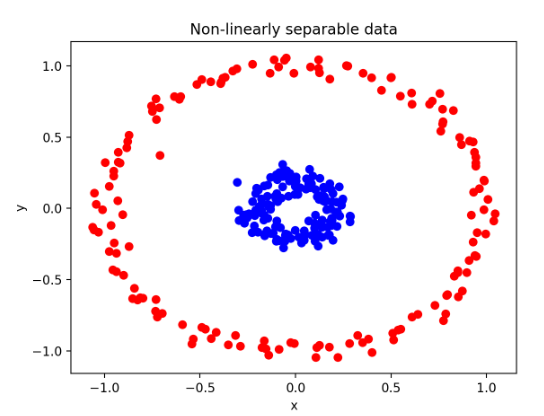
\includegraphics[scale=.5]{pk}
	\end{minipage}
	\begin{minipage}[c]{9cm}
		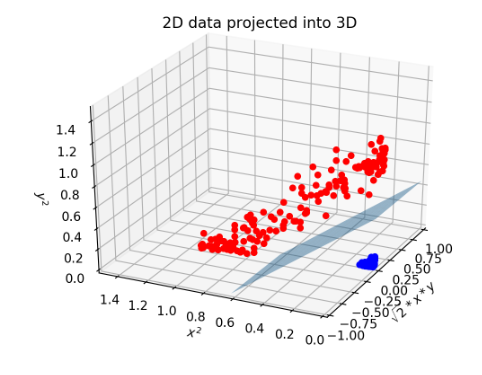
\includegraphics[scale=.5]{pk2}
	\end{minipage}
	\begin{lstlisting}
	classifier = SVC(kernel = "linear", random_state = 1)
	classifier.fit(training_data, training_labels)
	print(training_data[0]) # [0.31860062 0.11705731]
	print(classifier.score(validation_data, validation_labels)) # 0.56666666
	
	new_training = [[2**0.5 * point[0] * point[1], point[0]**2, point[1]**2] for 
	                point in training_data]
	
	new_validation = [[2**0.5 * point[0] * point[1], point[0]**2, point[1]**2] for 
	                  point in validation_data]
	
	classifier.fit(new_training, training_labels)
	print(new_training[0]) # [0.052742434610, 0.101506356208, 0.0137024148660]
	print(classifier.score(new_validation, validation_labels)) # 1.0 \end{lstlisting} \vspace*{1mm}
	The most commonly used kernel in SVMs is a \textbf{radial basis function} (rbf) kernel, which is the default kernel in scikit-learn. An rbf kernel transforms two-dimensional points into points with an infinite number of dimensions. You can essentially tune the model to be more or less sensitive to the training data by changing the \textit{gamma} parameter. High gamma make training data more important (but can cause overfitting) while low gamma makes training data less relevant (but can cause underfitting). 
	\begin{lstlisting}
	classifier = SVC(gamma = 1) # SVC object with rbf kernel
	classifier.fit(training_data, training_labels)
	print(classifier.score(validation_data, validation_labels)) # 0.8888888888 
	
	# note that a SVC with gamma 0.1 has a score of 0.777777777778 \end{lstlisting} \newpage
%%%% PAGE 91 %%%%

	\subsection{Decision Trees}
	\textbf{Decision trees} are machine learning models that try to find patterns in the features of data points. \vspace*{1mm} \\ 
	1) We begin with every point in the training set at the top of the tree. \\
	2) We then decide to split the data into smaller groups based on a feature. \\
	3) Once we have these subsets, we repeat the process - we split the data in each subset again on a \hspace*{4mm} different feature. \\
	4) Eventually, we reach a point where we decide to stop splitting the data into smaller groups. We’ve \hspace*{4mm} reached a leaf of the tree. We can now count up the labels of the data in that leaf. If an unlabeled \hspace*{4mm} point reaches that leaf, it will be classified as the \textit{majority label}. \vspace*{2mm} \\
	We want to end up at a leaf with only one type of label from the training data.	This idea can be quantified by calculating the \textbf{Gini impurity} of a set of data points. To find the Gini impurity, start at 1 and subtract the squared percentage of each label in the set. If a data set has only one class, you’d end up with a Gini impurity of 0. The lower the impurity, the better the decision tree.
	\begin{lstlisting}
	from collections import Counter
	
	labels = ["unacc", "unacc", "acc", "acc", "good", "good"]
	
	impurity = 1
	label_counts = Counter(labels)
	print(label_counts) # Counter({'unacc': 2, 'acc': 2, 'good': 2})
	for label in label_counts:
		probability_of_label = label_counts[label] / len(labels)
		impurity = impurity - probability_of_label ** 2
	print(impurity) # 0.6666666666666665 \end{lstlisting} \vspace*{1mm}
	We know that we want to end up with leaves with a low Gini Impurity, but we still need to figure out which features to split on in order to achieve this. To answer this question, we can calculate the \textbf{information gain} of splitting the data on a certain feature, which measures difference in the impurity of the data before and after the split. \vspace*{2mm} \\
	The sizes of the subset that get created after the split are important too. Let’s modify the formula for information gain to reflect the fact that the size of the set is relevant. Instead of simply subtracting the impurity of each set, we’ll subtract the \textbf{weighted impurity} of each of the split sets. $$ Weighted\; Information\; Gain\; = Base\; Impurity - Leaf\; Weight * Leaf\; Impurity\; ... $$ Note that we find the \textit{Leaf Weight * Leaf Impurity} for all features that we split on. \vspace*{2mm} \\
	The \textbf{sklearn.tree} module contains the \textit{DecisionTreeClassifier} class. Note that when building the tree with \textit{.fit()} we should map string values to numbers for our data points. 
	\begin{lstlisting}
	from cars import training_points, training_labels, testing_points, testing_labels
	from sklearn.tree import DecisionTreeClassifier
	
	print(training_points[0]) # [4.0, 3.0, 4.0, 2.0, 1.0, 2.0]
	print(training_labels[0]) # acc
	
	classifier = DecisionTreeClassifier() # create the object
	classifier.fit(training_points, training_labels) # build the tree
	print(classifier.score(testing_points, testing_labels)) # 0.97109826589	\end{lstlisting} \vspace*{1mm}
	One problem with the way we’re currently making our decision trees is that our trees aren’t always \textit{globablly optimal}. This means that there might be a better tree out there that produces better results. Our current strategy of creating trees is greedy. We assume that the best way to create a tree is to find the feature that will result in the largest information gain right now and split on that feature. \newpage
%%%% PAGE 92 %%%%

	\noindent Another problem with our trees is that they potentially \textit{overfit} the data. This means that the structure of the tree is too dependent on the training data and doesn’t accurately represent the way the data in the real world looks like. In general, larger trees tend to overfit the data more. \vspace*{2mm} \\
	One way to solve this problem is to \textbf{prune} the tree. The goal of pruning is to shrink the size of the tree. Scikit-learn currently doesn’t prune the tree by default, however we can dig into the code a bit to prune it ourselves. (Note in the below code that the accuracy increased when setting the max depth). 
	\begin{lstlisting}
	classifier = DecisionTreeClassifier(random_state = 0)
	classifier.fit(training_points, training_labels)
	print(classifier.score(testing_points, testing_labels)) # 0.97687861271
	print(classifier.tree_.max_depth) # 12
	
	classifier2 = DecisionTreeClassifier(random_state = 0, max_depth = 11)
	classifier2.fit(training_points, training_labels)
	print(classifier2.score(testing_points, testing_labels)) # 0.9826589595
	print(classifier2.tree_.max_depth) # 11	\end{lstlisting} \vspace*{1mm}
	Key ideas from lesson: \\
	- Good decision trees have \textbf{pure leaves}. A leaf is pure if all of the data points in that class have the \hspace*{2mm} same label. \\
	- An \textbf{internal node} represents which features to split the data on. \\
	- Decision trees are created using a \textbf{greedy algorithm} that prioritizes finding the feature that results \hspace*{2mm} in the largest information gain when splitting the data using that feature. \\
	- Decision trees often suffer from \textit{overfitting}. Making the tree small by \textbf{pruning} helps to generalize the \hspace*{2mm} tree so it is more accurate on data in the real world. \vspace*{1mm} \\
	DECISION TREE PROJECT. For more information (how the Landmass feature is stored) \href{http://archive.ics.uci.edu/ml/datasets/Flags}{click here}.
	\begin{lstlisting}
	flags = pd.read_csv('flags.csv', header = 0) # we want row 0 to be our header
	
	labels = flags['Landmass']
	data = flags[["Red", "Green", "Blue", "Gold", "White", "Black", "Orange", "Circles", 
	              "Crosses", "Saltires", "Quarters", "Sunstars", "Crescent", "Triangle"]]
	
	train_data, test_data, train_labels, test_labels = train_test_split(data, labels, 
	                                                   random_state = 1)
	
	scores = []
	for i in range(1,21): # try tree depth from 1 to 20
		tree = DecisionTreeClassifier(random_state = 1, max_depth = i)
		tree.fit(train_data, train_labels)
		scores.append(tree.score(test_data, test_labels))
	
	plt.plot(range(1,21), scores)
	plt.show()	# plot accuracy over the tree depth range (peak between 3 to 6)\end{lstlisting} \vspace*{1mm}
	
	\subsubsection{Random Forests}
	A \textbf{random forest} is an ensemble machine learning technique - a random forest contains many decision trees that all work together to classify new points. When a random forest is asked to classify a new point, the random forest gives that point to each of the decision trees. Each of those trees reports their classification and the random forest returns the most popular classification. It’s like every tree gets a vote, and the most popular classification wins. This can help solve the problem of \textit{overfitting} that often occures in decision trees by minimizing the impact these overfit estimations have in total. \newpage
%%%% PAGE 93 %%%%

	\noindent Random forests create different trees using a process known as \textbf{bagging}. Every time a decision tree is made, it is created using a different subset of the points in the training set (note that we chose these random rows \textit{with replacement}).  
	\begin{lstlisting}
	tree = build_tree(car_data, car_labels) # split on 'Estimated Safety'
	
	indices = [random.randint(0,999) for x in range(0,1000)] # 1000 random numbers
	
	data_subset = [car_data[index] for index in indices] # data at all indices
	labels_subset = [car_labels[index] for index in indices] # labels at all indices
	
	subset_tree = build_tree(data_subset, labels_subset) # split on 'Person Capacity' \end{lstlisting} \vspace*{1mm}
	Right now when we create a decision tree, we look at every one of those features and choose to split the data based on the feature that produces the most information gain. We could change how the tree is created by only allowing a subset of features to be considered at each split, known as \textbf{feature bagging}. To determine the \textbf{number of features to randomly select}, a good rule of thumb is to randomly select the \textit{square root} of the total number of features.
	\begin{lstlisting}
	unlabeled_point = ['high', 'vhigh', '3', 'more', 'med', 'med']
	
	predictions = []
	for x in range(0,20): # create 20 different trees
		indices = [random.randint(0, 999) for i in range(1000)] # random indices
		data_subset = [car_data[index] for index in indices] # random data
		labels_subset = [car_labels[index] for index in indices] # corresponding labels
		subset_tree = build_tree(data_subset, labels_subset) # build tree for forest
		predictions.append(classify(unlabeled_point, subset_tree)) # add prediction to list
	
	final_prediction = max(predictions, key=predictions.count) # find most common element
	print(final_prediction) # print result -> 'acc'	\end{lstlisting} \vspace*{1mm}
	\textbf{Scikit-learn} has a \textit{RandomForestClassifier} class that can create a given amount of decision trees for you, with all functions working similar to the DecisionTree class. 
	\begin{lstlisting}
	from cars import training_points, training_labels, testing_points, testing_labels
	from sklearn.ensemble import RandomForestClassifier
	
	classifier = RandomForestClassifier(n_estimators = 2000, random_state = 0)
	# note that n_estimators is the number of trees in the forest
	classifier.fit(training_points, training_labels)
	print(classifier.score(testing_points, testing_labels)) # 0.9826589595375722\end{lstlisting} \vspace*{1mm}
	PREDICTING INCOME WITH RANDOM FORESTS PROJECT
	\begin{lstlisting}
	income_data = pd.read_csv('income.csv', header=0, delimiter = ", ")
	
	income_data['sex-int'] = income_data['sex'].apply(lambda x : 0 if x == 'Male' else 1)
	income_data['country-int'] = income_data['native-country'].apply(lambda x : 0 if 
	                             x == 'United-States' else 1)
	
	labels = income_data[['income']]
	data = income_data[["age", "capital-gain", "capital-loss", "hours-per-week", 
	                    "sex-int", "country-int"]]
	
	train_data, test_data, train_labels, test_labels = train_test_split(data, labels, 
	                                                   random_state = 1)
	
	forest = RandomForestClassifier(random_state = 1)
	forest.fit(train_data, train_labels)
	print(forest.feature_importances_) # [0.3221 0.2906 0.1185 0.2004 0.0587 0.0097]
	print(forest.score(test_data, test_labels)) # 0.823731728288908 \end{lstlisting} \newpage
%%%% PAGE 94 %%%%

	\subsection{Classification: Naive Bayes}
	\subsubsection{Bayes' Theorem}
	\textbf{Bayes’ Theorem} is the basis of a branch of statistics called \textit{Bayesian Statistics}, where we take prior knowledge into account before calculating new probabilities. The general formula is: $$ P(A|B) = \frac{P(B|A) * P(A)}{P(B)} $$
	If two events are \textbf{independent}, then the occurrence of one event does not affect the probability of the other event. If two events are \textbf{dependent}, then when one event occurs, the probability of the other event occurring changes in a predictable way. \vspace*{1mm} \\
	\textbf{Conditional probability} is the probability that two events happen. It’s easiest to calculate conditional probability when the two events are independent. If event A and event B are independent, then the probability of both events occurring is the product of the probabilities: $$ P(A \cap B) = P(A) * P(B) $$ 
	The extra information about how we expect the world to work is called a \textbf{prior}. When we only use the first piece of information, it’s called a \textbf{Frequentist Approach} to statistics. When we incorporate our prior, it’s called a \textbf{Bayesian Approach}. Refer above for the general formula. \vspace*{1mm} \\
	ex: Suppose we are testing for a rare disease. We know the test is correct 99\% of the time and only $\frac{1}{100000}$ patients have it. Find P(rare disease $|$ positive result).
	\begin{lstlisting}
	p_positive_given_disease = 0.99 # P(B|A)
	p_disease = 1.0/100000 # P(A)
	p_positive = (p_disease * 0.99) + ((1-p_disease) * 0.01) #P(B)
	
	p_disease_given_positive = (p_positive_given_disease * p_disease) / p_positive
	print(p_disease_given_positive) # 0.000989030749865	\end{lstlisting} \vspace*{1mm}
	We can use Bayes' Theorem to determine \textbf{Spam Filters}. ex: Given that an email contains “enhancement”, what is the probability that the email is spam? We know “enhancement” appears in 0.1\% of non-spam emails, 5\% of spam emails, and that spam emails make up about 20\% of total emails.
	\begin{lstlisting}
	# let A = spam, B= enhancement
	
	p_spam = 0.20 # P(A)
	p_enhancement_given_spam = 0.05 #P(B|A)
	p_enhancement = (p_enhancement_given_spam * p_spam) + ( 0.001 * (1 - p_spam))
	# p_enhancement = P(B|A) * P(A) + P(B| not A) * P(not A) 
	
	p_spam_enhancement = (p_enhancement_given_spam * p_spam) / p_enhancement
	print(p_spam_enhancement) # 0.925925925926	\end{lstlisting} \vspace*{1mm}
	ex: Let event A = student knows the material, event B = answering correctly. Find P(A$|$B). We know: \\
	1) There is a question on the exam that 60\% of students know the correct answer to. \\
	2) Given a student knows the correct answer, there is a 15\% chance the student picked the wrong answer.\\
	3) Given a student doesn't know the answer, there is a 20\% chance the student guesses correctly.	
	\begin{lstlisting}
	p_knows_material = 0.60
	p_correct_given_knows_material = 1 - 0.15
	p_answering_correctly = (p_knows_material * p_correct_given_knows_material) + ((1-p_knows_material) * 0.20)
	
	bayes = (p_correct_given_knows_material * p_knows_material) / p_answering_correctly
	print(bayes) # 0.864406779661	\end{lstlisting} \newpage
%%%% PAGE 95 %%%%

	\subsubsection{Naive Bayes Classifier}
	A \textbf{Naive Bayes classifier} is a supervised machine learning algorithm that leverages Bayes’ Theorem to make predictions and classifications. Recall Bayes' formula from the previous section, this can be turned into a classifier if we replace B with a \textit{data point} and A with a \textit{class}. Naive Bayes classifiers are often used for text classification. In order to compute the probabilities used in Bayes’ theorem, we need previous data points. \vspace*{1.5mm} \\
	In this lesson, we are going to create a Naive Bayes classifier that can predict whether a review for a product is positive or negative. We labeled all reviews with a score less than 4 as a negative review. We have counter objects for the number of times a word appeared in the each of the positive and negative reviews. We want to classify: review = ``This crib was amazing". $$ P(positive | review) = \frac{P(review | positive) * P(positive)}{P(review)} $$
	The first part of Bayes’ Theorem that we are going to tackle is \textbf{P(positive)}. To find this, we need to look at all of our reviews in our dataset - both positive and negative - and find the percentage of reviews that are positive.
	\begin{lstlisting}
	from reviews import neg_list, pos_list, neg_counter, pos_counter

	total_reviews = len(pos_list) + len(neg_list)
	percent_pos = len(pos_list) / total_reviews
	percent_neg = len(neg_list) / total_reviews
	print(percent_pos) # P(positive) = 0.5
	print(percent_neg) # P(negative) = 0.5 \end{lstlisting} \vspace*{1mm}
	The second part of Bayes’ Theorem is a bit extensive. We now want to compute \textbf{P(review $|$ positive)}. Let positive be abbreviated to pos. To do this, we must find: \\ P(“This crib was amazing"$|$pos) = P(“This"$|$pos)*P(“crib"$|$pos)*P(“was"$|$pos)*P(“amazing"$|$pos). \vspace*{1.5mm} \\
	We will use a technique called \textbf{smoothing} to avoid multiplying by 0 if the word we are looking for does not exist in any of our positive reviews. In this case, we smooth by adding \textit{1} to the numerator of each probability and \textit{N} (number of unique words in our dataset) to the denominator of each probability. 
	\begin{lstlisting}
	total_pos = sum(pos_counter.values()) # total number of positive reviews
	total_neg = sum(neg_counter.values()) # total number of negative reviews
	pos_probability, neg_probability = 1, 1 # probability starts at 1
	review_words = review.split() # create list of review words
	
	for word in review_words:
		word_in_pos = pos_counter[word]
		word_in_neg = neg_counter[word]
		pos_probability *= (word_in_pos + 1) / (total_pos + len(pos_counter))
		neg_probability *= (word_in_neg + 1) / (total_neg + len(neg_counter))
	
	print(pos_probability) # P(review|positive) = 7.684476462488163e-13
	print(neg_probability) # P(review|negative) = 2.389642284511267e-13	\end{lstlisting} \vspace*{1mm}
	Before we compute \textbf{P(review)}, think of our original question. We want to predict whether the review is positive or negative. The value for P(review) is the same in both cases, so there’s no reason why we need to divide them by the same value. This means we can completely \textbf{ignore the denominator}. 
	\begin{lstlisting}
	final_pos = pos_probability * percent_pos
	final_neg = neg_probability * percent_neg
	if final_pos > final_neg:
		print('The review is positive') # This statement is printed
	else:
		print('The review is negative')	\end{lstlisting} \newpage
%%%% PAGE 96 %%%%
	
	\noindent  In order to use scikit-learn’s Naive Bayes classifier, we need to first \textbf{transform our data} into a format that scikit-learn can use. A \textbf{tagged} dataset is necessary to calculate the probabilities used in Bayes’ Theorem. To do so, we’re going to use scikit-learn’s \textit{CountVectorizer} object. \\
	1) We need to teach it the vocabulary of the training set by calling the .fit() method. \\
	2) After fitting the vectorizer, we can now call .transform() which takes a list of strings and will transform \hspace*{3mm} those strings into counts of the trained words (use .vocabulary\_ to see the index of each word). \\
	3) We than use the varaible storing the .transform( ) value as our input to our Naive Bayes Classifier. 
	\begin{lstlisting}
	from reviews import neg_list, pos_list
	from sklearn.feature_extraction.text import CountVectorizer
	
	review = "This crib was amazing"
	
	counter = CountVectorizer()
	counter.fit(neg_list + pos_list)
	review_counts = counter.transform([review])
	training_counts = counter.transform(neg_list + pos_list)\end{lstlisting} \vspace*{1mm}
	Now that we’ve formatted our data correctly, we can use it using \textbf{scikit-learn} \textit{MultinomialNB} classifier. Note that the .predict\_proba( ) method prints the probability of the data being each label (in this case, bad or good). The class with the highest probability will be the algorithm’s prediction.
	\begin{lstlisting}
	from sklearn.naive_bayes import MultinomialNB
	
	review = "This crib was great amazing and wonderful"
	review_counts = counter.transform([review]) # counts for reviews (must be a list)
	training_labels = [0] * 1000 + [1] * 1000 # create our labels
	
	classifier = MultinomialNB() # create object
	classifier.fit(training_counts, training_labels) # train the model
	print(classifier.predict(review_counts)) # [1] meaning good review
	print(classifier.predict_proba(review_counts)) # [[0.04977729 0.95022271]] \end{lstlisting} \vspace*{1mm}
	Some methods used to \textbf{improve data} before feeding into the classifier (Natural Language Processing Techniques): \\
	\hspace*{3mm} - Remove punctuation from the training set. \\
	\hspace*{3mm} - Lowercase every word in the training set. \\
	\hspace*{3mm} - Using a bigram model makes the assumption of independence more reasonable. 
	\begin{lstlisting}
	from sklearn.datasets import fetch_20newsgroups
	from sklearn.naive_bayes import MultinomialNB
	from sklearn.feature_extraction.text import CountVectorizer
	
	train_emails = fetch_20newsgroups(categories = ['comp.sys.ibm.pc.hardware','rec.
	               sport.hockey'], subset = 'train', shuffle = True, random_state = 108)
	test_emails = fetch_20newsgroups(categories = ['comp.sys.ibm.pc.hardware','rec.
	               sport.hockey'], subset = 'test', shuffle = True, random_state = 108)
	
	counter = CountVectorizer()
	counter.fit(test_emails.data + train_emails.data) # .data holds the email contents
	train_counts = counter.transform(train_emails.data)
	test_counts = counter.transform(test_emails.data)
	
	classifier = MultinomialNB()
	classifier.fit(train_counts, train_emails.target) # .target has the labels (0, 1)
	print(classifier.score(test_counts, test_emails.target)) # 0.9974715549936789 \end{lstlisting} \newpage
%%%% PAGE 97 %%%%

	\subsection{AI Decision Making: Minimax}
	The concept of thinking ahead is the central idea behind the \textbf{minimax algorithm}. The minimax algorithm is a decision-making algorithm that is used for finding the best move in a two player game (it’s a recursive algorithm). Think of this as a \textit{tree} with the lead nodes being the possible outcomes of the game. In order to determine which move to make, we’d guess what our opponent would do by running the minimax algorithm from our opponent’s point of view. The recursion stops when the game is over (either we won or the opponent did). \vspace*{2mm} \\
	For the rest of this exercise, we will write the minimax algorithm to be used on a game of Tic-Tac-Toe. An essential step in the minimax function is evaluating the \textbf{strength} of a leaf (we want to know which player had the better outcome). Here’s one potential \textit{evaluation function}: a leaf where player ``X" wins evaluates to a 1, a leaf where player ``O" wins evaluates to a -1, and a leaf that is a tie evaluates to 0. \vspace*{2mm} \\
	Now we move onto \textbf{evaluating} the leaves. Let's say were playing as the ``X" player and you have 3 choices, picking move A will result in you winning and moves B/C will each result in a tie. By picking move A, you’ve picked the move that led to the board with the \textit{highest value} (1) and are now the \textbf{maximizing player}. Let's say were playing as the ``O" player instead and you have 3 choices, picking move A would somehow immediately lead to you losing, while moves B and C would lead to a tie. You’d pick one of the boards that would lead to a tie (0) and become the \textbf{minimizing player} (you'd ideally want to chose -1 but it was not an option). \vspace*{2mm} \\
	One of the central ideas behind the minimax algorithm is the idea of \textbf{exploring future hypothetical states}. Essentially, we’re saying if we were to make this move, what would happen. We don’t want to actually make our move on the board but rather make a copy of the board and make the move on that one. In order to do this, we must use \textit{deepcopy( )} to make a copy of the board in a different place in memory (\textit{from copy import deepcopy}).
	\begin{lstlisting}
	def minimax(input_board, is_maximizing):
		if game_is_over(input_board): # base case
			return [evaluate_board(input_board), ""] # returns (1, 0, or -1) and ""
		best_move = ""
		if is_maximizing == True: # if player 'X' turn
			best_value = -float("Inf") # set smallest value possible
			symbol = "X"
		else: # player 'O' turn
			best_value = float("Inf") # set biggest value possible
			symbol = "O"
		for move in available_moves(input_board): # try all available moves
			new_board = deepcopy(input_board) # create new copy in memory
			select_space(new_board, move, symbol) # make move on the copy
			# this recursive call below is with the new move and for the opposite player
			hypothetical_value = minimax(new_board, not is_maximizing)[0] # returns list
			if is_maximizing and hypothetical_value > best_value: # better move for 'X'
				best_value = hypothetical_value
				best_move = move
			if not is_maximizing and hypothetical_value < best_value: # better move for 'O'
				best_value = hypothetical_value
				best_move = move
		return [best_value, best_move] # return list of value and move \end{lstlisting} \vspace*{1mm}
	Key takeaways from this lesson: \\
	1) A game can be represented as a tree. The current state of the game is the root of the tree, and each potential move is a child of that node. The leaves of the tree are game states where the game has ended. \\
	2) The minimax algorithm returns the best possible move for a given game state. It assumes that your opponent will also be using the minimax algorithm to determine their best move. \\
	3) Game states can be evaluated and given a specific score (in this case: -1, 0, or 1). \newpage
%%%% PAGE 98 %%%%

	\section{Machine Learning (Unsupervised Learning)}
	\subsection{K-Means Clustering}
	\textbf{Unsupervised Learning} is how we find patterns and structure in \textit{unlabeled} data that don't provide labeled answers to your question. \textbf{Clustering} finds structure in unlabeled data by identifying similar groups, or clusters. Some examples are recommendation/search engines or market/image segmentation. \\~\\
	The goal of clustering is to separate data so that data similar to one another are in the same group, while data different from one another are in different groups. But how many groups do we chose? \textbf{K-Means} is the most popular and well-known clustering algorithm: \\
	\hspace*{3mm}- The ``K" refers to the number of clusters (groups) we expect to find in a dataset. \\
	\hspace*{3mm}- The ``Means'' is the average distance of data to each cluster center (centroid), we want to minimize. \vspace*{1mm} \\
	The \textbf{steps} we take are iterative: \\
	\hspace*{3mm} 1) Place k random centroids for the initial clusters. \\
	\hspace*{3mm} 2) Assign data samples to the nearest centroid. \\
	\hspace*{3mm} 3) Update centroids based on the above-assigned data samples. \vspace*{1mm} \\
	Repeat Steps 2/3 until \textbf{convergence} (when points don’t move between clusters and centroids stabilize).\\~\\
	We can \textbf{import datasets from sklearn} to use in our projects. We can use the following accessors: \\
	\hspace*{3mm}- \textit{.data} : lets us view the sample data of our module.\\
	\hspace*{3mm}- \textit{.target} : gives us the answers (labels) for the corresponding data. \\
	\hspace*{3mm}- \textit{.DESCR} : gives us features (columns), class (labels), summary statistics, and more. 
	\begin{lstlisting}
	from sklearn import datasets
	
	iris = datasets.load_iris() # an example of this data is : [5.6 2.7 4.2 1.3] \end{lstlisting} \vspace*{1mm}
	We will start by implementing \textbf{step 1} using the iris dataset. We expect 3 clusters (for 3 flower species). 
	\begin{lstlisting}
	samples = iris.data # get only the data from our dataset
	
	x = samples[:,0] # all rows, sepal length column
	y = samples[:,1] # all rows, sepal width column
	
	k = 3 # Number of clusters (classes)
	centroids_x = np.random.uniform(min(x), max(x), size=k) # 3 random x centroids
	centroids_y = np.random.uniform(min(y), max(y), size=k) # 3 random y centroids
	centroids = np.array(list(zip(centroids_x, centroids_y))) # centroid matrix (3x2) \end{lstlisting} \vspace*{1mm}
	We will now implement \textbf{step 2}. We will assign data points to the nearest centroid using the Distance Formula. We will have a list of 3 distances and use \textit{argmin( )} to find the smallest index.
	\begin{lstlisting}
	def distance(a,b): # Distance formula
		dis = sum([(a-b)**2 for a,b in zip(a,b)]) ** 0.5
		return dis
	
	labels = np.zeros(len(samples)) # Cluster labels for each point (init to 0)
	distances = np.zeros(k) # [0 0 0]
	
	for i in range(len(samples)): # go through all samples
		distances[0] = distance(sepal_length_width[i], centroids[0])
		distances[1] = distance(sepal_length_width[i], centroids[1])
		distances[2] = distance(sepal_length_width[i], centroids[2])
		cluster = np.argmin(distances) # get the smallest distance index
		labels[i] = cluster # assign data point its corresponding label (0,1,2) \end{lstlisting} \newpage
%%%% PAGE 99 %%%%
	
	\noindent We will now implement \textbf{step 3}. Find new cluster centers by taking the average of the assigned points.
	\begin{lstlisting}
	from copy import deepcopy
	
	centroids_old = deepcopy(centroids) 
	for x in range(k): # iterate 3 times
		points = [sepal_length_width[j] for j in range(len(sepal_length_width)) 
		          if labels[j] == x] # get data point if labels match
		centroids[x] = np.mean(points, axis = 0) # mean of points with same cluster label \end{lstlisting} \vspace*{1mm}
	We will now \textbf{repeat steps 2/3} until the centroids stabilize (convergence). We stop when all three values in our error array are equal to 0 (difference between old and new centroid). Place the code from steps 2 and 3 inside the while loop.
	\begin{lstlisting}
	error = np.zeros(3)
	for x in range(3):
		error[x] = distance(centroids[x], centroids_old[x]) # find initial distance
		
	while error.all() != 0: # while not all index values are 0
		for i in range(len(samples)):
			distances[0] = distance(sepal_length_width[i], centroids[0])
			distances[1] = distance(sepal_length_width[i], centroids[1])
			distances[2] = distance(sepal_length_width[i], centroids[2])
			cluster = np.argmin(distances)
			labels[i] = cluster
		
		centroids_old = deepcopy(centroids)
		for i in range(3):
			points = [sepal_length_width[j] for j in range(len(sepal_length_width)) 
			          if labels[j] == i]
			centroids[i] = np.mean(points, axis=0)
		
		for x in range(3):
			error[x] = distance(centroids[x], centroids_old[x]) # find new distance	\end{lstlisting} \vspace*{1mm}
	We can now use the \textbf{sklearn.cluster} module to implement K-Means more efficiently. After this, we can feed new data samples into it and obtain cluster labels using \textit{.predict( )}. 
	\begin{lstlisting}
	from sklearn.cluster import KMeans
	
	model = KMeans(n_clusters = 3) # create model with k clusters
	model.fit(samples) # compute K-Means clustering
	labels = model.predict(samples) # compute cluster centers and index for each sample	
	
	new_samples = np.array([[5.7, 4.4, 1.5, 0.4],
	                        [6.5, 3. , 5.5, 0.4],
	                        [5.8, 2.7, 5.1, 1.9]])
	 
	print(model.predict(new_samples)) # [1 2 2], labels for each row \end{lstlisting} \vspace*{1mm}
	We now must \textbf{evaluate} our model to see if it correctly clustered the data. We change these values into the corresponding species and then use Pandas to perform a \textbf{cross-tabulation}, which enable you to examine relationships within the data and see the accuracy of our predictions. We know: \\
	\hspace*{3mm} - All the 0's are Iris-setosa. \\
	\hspace*{3mm} - All the 1's are Iris-versicolor. \\
	\hspace*{3mm} - All the 2‘s are Iris-virginica. \newpage
%%%% PAGE 100 %%%%

	\begin{lstlisting}
	target = iris.target # get all labels
	species = np.chararray(target.shape, itemsize=150)
	
	for i in range(len(samples)): # 
		if target[i] == 0:
			species[i] = 'setosa'
		elif target[i] == 1:
			species[i] = 'versicolor'
		elif target[i] == 2: 
			species[i] = 'virginica'

	# create df will labels and corresponding species name
	df = pd.DataFrame({'labels': labels, 'species': species})
	
	ct = pd.crosstab(df['labels'], df['species'])
	print(ct)
	# species  b'setosa'  b'versicolor'  b'virginica'
	# labels                                         
	# 0               50              0             0
	# 1                0             48            14
	# 2                0              2            36 \end{lstlisting} \vspace*{1mm}
	What is the best number of clusters and how do we determine that? \textbf{Good clustering} results in tight clusters, meaning that the samples in each cluster are bunched together. How spread out the clusters are is measured by \textbf{inertia}, which is the distance from each sample to the centroid of its cluster. The lower the inertia is, the better our model has done. We can check this with \textit{.inertia\_} on our model. \vspace*{1mm} \\
	One of the ways to interpret this graph is to use the \textbf{elbow method}, when inertia begins to decrease more slowly on the plot. \\
	\begin{minipage}[c]{9cm}
	\begin{lstlisting}
	num_clusters = list(range(1,9))
	inertias = []
	
	for k in num_clusters:
	model = KMeans(n_clusters = k)
	model.fit(samples)
	inertias.append(model.inertia_)
	
	plt.plot(num_clusters, inertias, '-o')
	plt.xlabel('Number of Clusters (k)')
	plt.ylabel('Inertia')
	plt.show() # we see 3 is the optimal choice \end{lstlisting} \vspace*{1mm}
	\end{minipage}
	\begin{minipage}[c]{9cm}
	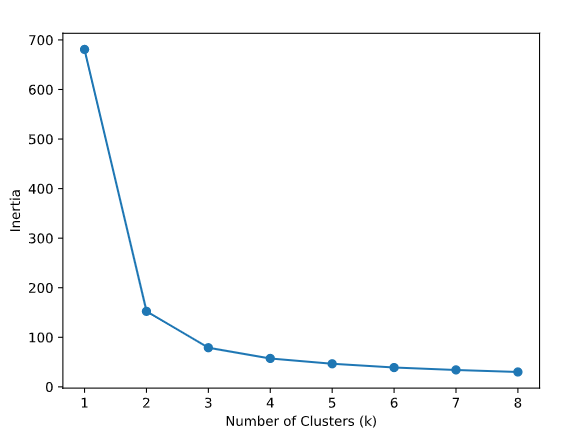
\includegraphics[scale=.53]{inertia}
	\end{minipage} \\
	
	\noindent In the traditional K-Means algorithms, the starting positions of the centroids are initialized completely randomly. This can result in sub-optimal clusters. \textbf{K-Means++} changes the way centroids are initialized to try to fix this problem. \vspace*{2mm} \\
	The K-Means++ algorithm replaces Step 1 of the K-Means algorithm and adds the following: \\
	\hspace*{2mm} 1.1) The first cluster centroid is randomly picked from the data points. \\
	\hspace*{2mm} 1.2) For each remaining data point, find the distance from the point to its nearest cluster centroid. \\
	\hspace*{2mm} 1.3) The next cluster centroid is picked according to a probability proportional to the distance of each \hspace*{10mm} point to its nearest cluster centroid. This makes it likely for the next cluster centroid to be far \hspace*{10mm} away from the already initialized centroids. Repeat 1.2/1.3 until k centroids are chosen. \vspace*{2mm} \\
	We can use the \textbf{sklearn.cluster} module similarly to the K-Means algorithm, but when initializing our model we pass init=`k-means++'. Note that this is actually the default parameter, and if you wanted to use the original K-Means clustering method you would pass init=`random' to the model. \newpage
%%%% PAGE 101 %%%%

	\section{Advanced Machine Learning Topics}
	\subsection{Perceptrons and Neural Nets}
	A \textbf{neural network} is a programming model that simulates the human brain. The \textbf{Perceptron} algorithm allows an artificial neuron to simulate a biological neuron. The artificial neuron could take in an input, process it based on some rules, and fire a result. This was impressive because the artificial neuron could train itself based on its own results, and fire better results in the future (learn by trial and error). \vspace*{1.5mm} \\
	It was found out that creating multiple layers of neurons - with one layer feeding its output to the next layer as input - could process a wide range of inputs, make complex decisions, and still produce meaningful results. With some tweaks, the algorithm became known as the \textbf{Multilayer Perceptron}, also known as a \textit{Feedforward Neural Network}. \vspace*{2mm} \\
	The perceptron has three main components: \\
	1) \textbf{Inputs} - each input corresponds to a feature. \\
	2) \textbf{Weights} - each input also has a weight which assigns a certain amount of importance to the input. \\
	3) \textbf{Output} - the perceptron uses the inputs and weights to produce an output. The type of the output \hspace*{21mm} varies depending on the nature of the problem (can be binary, a range, etc.). \vspace*{2mm} \\
	The first step is to find the \textbf{weighted sum}, which is found by: $x_1w_1 + x_2w_2 + ... + x_nw_n$ \vspace*{1.5mm} \\
	The second step is to constrain the weighted sum to produce a desired output through an \textbf{activation function}. For example, if you want to train a perceptron to detect whether a point is above or below a line, you might want the output to be a +1 or -1 label. We would want our function to return +1 if the weight sum is positive, or -1 if the weight sum is negative. 
	\begin{lstlisting}
	class Perceptron:
		def __init__(self, num_inputs=2, weights=[1,1]):
			self.num_inputs = num_inputs
			self.weights = weights
		
		def weighted_sum(self, inputs):
			weighted_sum = sum([self.weights[i] * inputs[i] for i in range(self.num_inputs)])
			return weighted_sum
		
		def activation(self, weighted_sum):
			if weighted_sum >= 0:
				return 1
			else:
				return -1 \end{lstlisting} \vspace*{1mm}
	We must provide the perceptron a \textbf{training set}, a collection of random inputs with correctly predicted outputs, in order to get the perceptron to produce accurate results (compare against the expected labels). Every time the output mismatches the expected label, we say that the perceptron has made a \textbf{training error}, a quantity that measures ``how bad" the perceptron is performing. We find this value by subtracting the predicted label value from the actual label value. \vspace*{1.5mm} \\
	The goal is to nudge the perceptron towards zero training error. The only way to do that is to change the parameters that define the perceptron (the weights). We want to find the optimal combination of weights that will produce the correct output for as many points as possible in the dataset. \vspace*{1.5mm} \\
	The \textbf{Perceptron Algorithm} helps us optimally tweak the weights towards a zero training error. We use the \textit{update rule} where: weights = weight + (error*input). We keep on tweaking the weights until all possible labels are correctly predicted by the perceptron. \newpage
	\begin{lstlisting}
	# within our Perceptron class above, we define the training function
	def training(self, training_set):
		foundLine = False # whether the perceptron found a line to seperate the labels
			while not foundLine: # continue to train while no line found
			total_error = 0 # count the total error made in each round
			for inputs in training_set:
				prediction = self.activation(self.weighted_sum(inputs))
				actual = training_set[inputs]
				error = actual - prediction
				total_error += abs(error) # update total error each round
				for i in range(self.num_inputs):
					self.weights[i] += error * inputs[i] # update rule (change weights)
			if total_error == 0: # if all labels correctly predicted
				foundLine = True \end{lstlisting} \vspace*{1mm}
	There are times when a minor adjustment is needed for the perceptron to be more accurate. This supporting role is played by the \textbf{bias weight}. It takes a default input value of 1 and some random weight value. The new weighted sum equation is: $x_1w_1 + x_2w_2 + ... + x_nw_n + 1w_b$
	\begin{lstlisting}
	# the only thing that needs to be changed is in init method (add 1 input & weight)
	class Perceptron:
		def __init__(self, num_inputs=3, weights=[1,1,1]): \end{lstlisting} \vspace*{1mm}
	We can visualize the changing of weights throughout training by using them to \textbf{represent a line}. A perceptron’s weights can be used to find the slope and intercept of the line that the perceptron represents: \\
	\hspace*{4mm} slope = -self.weights[0] / self.weights[1] \\
	\hspace*{4mm} intercept = -self.weights[2] / self.weights[1] \vspace*{2mm} \\
	What does it mean for the perceptron to correctly classify every point in the training set? Tt means that the perceptron found a \textbf{linear classifier}, or a \textit{decision boundary}, that separates the two distinct set of points in the training set (when the data is linearly separable). \vspace*{1mm} \\
	A single perceptron with only two inputs wouldn't work for such a scenario because it cannot represent a non-linear decision boundary. By increasing the number of features and perceptrons, we can give rise to the \textbf{Multilayer Perceptrons}, also known as \textit{Neural Networks}. \vspace*{2mm} \\
	We can use the \textbf{sklearn} module to use a built in implementation of the Perceptron. Note that the default max\_iter (number of times it loops through the training data) is 1000. Also, the .decision\_function( ) method takes a list of points and returns the distance they are from the decision boundary. 
	\begin{lstlisting}
	from sklearn.linear_model import Perceptron
	from itertools import product
	
	data = [[0,0], [0,1], [1,0], [1,1]] # inputs for AND gate
	labels = [0, 0, 0, 1] # corresponding outputs for AND gate
	
	plt.scatter([p[0] for p in data], [p[1] for p in data], c = labels)
	
	classifier = Perceptron(max_iter = 40) # create model
	classifier.fit(data, labels) # train the model on our data
	
	x_values = np.linspace(0, 1, 100) # 100 evenly spaced decimals between 0 and 1
	y_values = np.linspace(0, 1, 100) # 100 evenly spaced decimals between 0 and 1
	point_grid = list(product(x_values, y_values)) # all possible combinations
	
	distances = classifier.decision_function(point_grid) # get distances from line
	abs_distance = [abs(x) for x in distances] # all values should be a positive distance
	distance_matrix = np.reshape(abs_distance, (100,100)) # reshape to 2D matrix
	
	heatmap = plt.pcolormesh(x_values, y_values, distance_matrix) # gradient visual
	plt.colorbar(heatmap) # add legend to our graph \end{lstlisting} \newpage
%%%% PAGE 103 %%%%

	\subsection{Natural Language Processing}
	\textbf{Natural Language Processing (NLP)} is the field is at the intersection of linguistics, artificial intelligence, and computer science by enabling computers to interpret, analyze, and approximate the generation of human languages. \vspace*{2mm} \\
	Cleaning and preparation are crucial for many tasks, and NLP is no exception. \textbf{Text preprocessing} is usually the first step you’ll take when faced with an NLP task. By using Regex and NLTK (Python's NLP library), we can do the following common tasks: \\
	\hspace*{2mm} - \textbf{Noise Removal} : stripping text of formatting (such as HTML tags). \\
	\hspace*{2mm} - \textbf{Tokenization} : breaking text into individual words. \\
	\hspace*{2mm} - \textbf{Normalization} : clean text data in any other way (including the following): \\
	\hspace*{8mm} 1) \textbf{Stemming} : chop off word prefixes and suffixes (`booing'/`booed' become `boo'). \\
	\hspace*{8mm} 2) \textbf{Lemmatization} : bring words down to their root forms (`am' and `are' related to `be').
	\begin{lstlisting}
	import re
	import nltk
	from nltk.tokenize import word_tokenize
	from nltk.stem import PorterStemmer
	from nltk.stem import WordNetLemmatizer
	from part_of_speech import get_part_of_speech # for lemmatization
	
	text = "So many squids are jumping out of suitcases these days that you can barely go 
	        anywhere without seeing one burst forth from a tightly packed valise. I went 
	        to the dentist the other day, and sure enough I saw an angry one jump out of 
	        my dentist's bag within minutes of arriving. She hardly even noticed."
	
	cleaned = re.sub('\W+', ' ', text) # remove non letter characters (. , ') 
	tokenized = word_tokenize(cleaned) # create list of each word
	
	stemmer = PorterStemmer() # create object
	stemmed = [stemmer.stem(token) for token in tokenized] # normalize text with stemming
	
	lemmatizer = WordNetLemmatizer() # create object
	lemmatized = [lemmatizer.lemmatize(token, get_part_of_speech(token)) for token in 
	              tokenized] # normalize text with lemmatization \end{lstlisting} \vspace*{1mm}
	We now have a preprocessed, clean list of words. \textbf{Parsing} is a stage of NLP concerned with segmenting text based on syntax (know how the words relate to each other and the underlying syntax). \\
	\hspace*{2mm} - \textbf{Part-of-speech tagging (POS tagging)} : identifies parts of speech (verbs, nouns, adjectives, etc). \\
	\hspace*{2mm} - \textbf{Named entity recognition (NER)} : help identify proper nouns in a text (helps with text topic).\\
	\hspace*{2mm} - \textbf{Dependency grammar trees} : understand the relationship between words in a sentence (\textit{spaCy}). \\
	\hspace*{2mm} - \textbf{Regex parsing} : find common patterns within large text chunks (with POS tagging -$>$ find phrases). \\~\\
	We can help computers make predictions about language by training a language model on a \textit{corpus} (a bunch of example text). \textbf{Language models} are probabilistic computer models of language. We build and use these models to figure out the likelihood that a given sound, letter, word, or phrase will be used. \\~\\
	One of the most common language models is the \textit{unigram model}, a statistical language model commonly known as \textbf{bag-of-words}. This model doesn't have much order but it has a tally count of each instance for each word (map each word to it's appearance count). Note that when grammar and word order are irrelevant, this is probably a good model to use. We can use a Python Counter object to turn a list of words into a bag-of-words. \newpage
%%%% PAGE 104 %%%%
	
	\noindent For parsing entire phrases or conducting language prediction, you will want to use a model that pays attention to each word’s neighbors. The \textbf{n-gram} model considers a sequence of some number (n) units and calculates the probability of each unit in a body of language given the preceding sequence of length n. The larger the n, the better the language prediction. \vspace*{1.5mm} \\
	Two issues can occur with the n-gram model: \\
	1) During training, your model will probably come across test words that it has never encountered \\ \hspace*{3mm} before. A tactic known as \textit{language smoothing} can help adjust probabilities for unknown words, but \hspace*{3mm} it isn’t always ideal. \\
	2) We want n to be as large as possible. As the sequence length grows, the number of examples of each \hspace*{3mm} sequence within your training corpus shrinks. With too few examples, you won’t have enough data to \hspace*{3mm} make many predictions. \vspace*{2mm} \\
	This can be fixed with \textbf{neural language models (NLM)}. Much recent work within NLP has involved developing and training neural networks to approximate the approach our human brains take towards language. This deep learning approach allows computers a much more adaptive tack to processing human language.
	\begin{lstlisting}
	import nltk, re
	from nltk.tokenize import word_tokenize
	from nltk.util import ngrams
	from collections import Counter
	from looking_glass import looking_glass_full_text
	
	cleaned = re.sub('\W+', ' ', looking_glass_full_text).lower()
	tokenized = word_tokenize(cleaned)
	
	looking_glass_bigrams = ngrams(tokenized, 2) # n-gram with n = 2 (known as bigram)
	looking_glass_bigrams_frequency = Counter(looking_glass_bigrams)  \end{lstlisting} \vspace*{1mm}
	\textbf{Topic modeling} is an area of NLP dedicated to uncovering latent, or hidden, topics within a body of language. A common technique is to deprioritize the most common words and prioritize less frequently used terms as topics in a process known as \textbf{term frequency-inverse document frequency (tf-idf)}. Note that the Python libraries \textit{gensim} and \textit{sklearn} have modules to handle tf-idf. \vspace*{1mm} \\
	The next step in your topic modeling journey is often \textbf{latent Dirichlet allocation (LDA)}. LDA is a statistical model that takes your documents and determines which words keep popping up together in the same contexts (we can use \textit{sklearn} for this). If you have any interest in visualizing your newly minted topics, \textbf{word2vec} can map out your topic model results spatially as vectors so that similarly used words are closer together. This word-to-vector mapping is known as a word \textit{embedding}.
	\begin{lstlisting}
	from sklearn.feature_extraction.text import CountVectorizer, TfidfVectorizer
	from sklearn.decomposition import LatentDirichletAllocation	\end{lstlisting} \vspace*{1mm}
	Addressing \textbf{text similarity}, including spelling correction, is a major challenge within natural language processing. Addressing word similarity and misspelling for spellcheck or auto correct often involves considering the \textbf{Levenshtein distance} or minimal edit distance between two words. The distance is calculated through the minimum number of insertions, deletions, and substitutions that would need to occur for one word to become another. Some other challenging similarities for NLP are: \\
	\hspace*{2mm} - \textbf{Phonetic similarity} : how much two words or phrases sound the same. \\
	\hspace*{2mm} - \textbf{Lexical similarity} : the degree to which texts use the same vocabulary and phrases (plagiarism). \\
	\hspace*{2mm} - \textbf{Semantic similarity} : the degree to which documents contain similar meaning/topics.
	\begin{lstlisting}
	from nltk.metrics import edit_distance # build in Levenshtein distance function	
	
	word_one, word_two = 'hello', 'help'
	print("The Levenshtein distance: {}".format(edit_distance(word_one, word_two))) 
	# The Levenshtein distance: 2 \end{lstlisting} \newpage
%%%% PAGE 105 %%%%
	
	\noindent \textbf{Language prediction} is an application of NLP concerned with predicting text given preceding text. Auto-suggest, auto complete, and suggested replies are common forms of language prediction. We must pick a language model for our prediction (these are the two most common): \vspace*{1mm} \\
	1) If you go the \textit{n-gram} route, you will most likely rely on \textbf{Markov chains} to predict the statistical likelihood of each following word (or character) based on the training corpus. Markov chains are memory-less and make statistical predictions based entirely on the current n-gram on hand. \vspace*{1mm} \\
	2) A more advanced approach, using a neural language model, is the \textbf{Long Short Term Memory (LSTM)} model. LSTM uses deep learning with a network of artificial “cells” that manage memory, making them better suited for text prediction than traditional neural networks.
	\subsubsection{Parsing with Regular Expressions}
	Before you dive into more complex syntax parsing, you’ll begin with basic regular expressions in Python using the \textbf{re module}. Lets take a look at a few methods we can use from this module: \\
	\hspace*{2mm} - \textit{.compile()} takes a re pattern and compiles into an object we can later use to find matching text. \\
	\hspace*{2mm} - \textit{.match()} looks for a single match to the re that starts at the beginning of the string.
	\begin{lstlisting}
	import re
	
	character_1 = "Dorothy"
	character_2 = "Henry"
	
	regular_expression = re.compile('[A-Za-z]{7}') # compile re
	result_1 = regular_expression.match(character_1) # check for match
	match_1 = result_1.group(0) # store match
	print(match_1) # Dorothy
	
	result_2 = re.match('[A-Za-z]{7}', character_2) # compile and check match
	print(result_2) # None	\end{lstlisting} \vspace*{1mm}
	Unlike the match function, \textbf{.search()} will look left to right through an entire piece of text and return a match object for the first match to the regular expression given. Similarly, \textbf{.findall()} will return a list of all non-overlapping matches of the regular expression in the string (not just the first like search does). 
	\begin{lstlisting}
	oz_text = open("the_wizard_of_oz_text.txt",encoding='utf-8').read().lower()
	
	found_wizard = re.search('wizard', oz_text) # search for an occurrence of 'wizard'
	print(found_wizard)
	
	all_lions = re.findall('lion', oz_text) # find all the occurrences of 'lion'
	number_lions = len(all_lions)
	print(number_lions)	\end{lstlisting} \vspace*{1mm}
	You can often find more meaning by analyzing text on a word-by-word basis, focusing on the part of speech of each word in a sentence. This process of identifying and labeling the part of speech of words is known as \textbf{part-of-speech tagging}. You can automate this process with NLTK's \textit{pos\_tag()} function, which takes a list of words in the order they appear in a sentence and returns a list of tuples (where the first entry in the tuple is a word and the second is the part-of-speech tag). \href{https://www.ling.upenn.edu/courses/Fall_2003/ling001/penn_treebank_pos.html}{Click here to see all tags}.
	\begin{lstlisting}
	import nltk
	from nltk import pos_tag
	from word_tokenized_oz import word_tokenized_oz
		
	pos_tagged_oz = []
	for word in word_tokenized_oz: # go through each tokenized word
		pos_tagged_oz.append(pos_tag(word)) # append part-of-speech tag
	
	print(pos_tagged_oz[100]) # [('the', 'DT'), ('house', 'NN'), ('must', 'MD'), 
	# ('have', 'VB'), ('fallen', 'VBN'), ('on', 'IN'), ('her', 'PRP'), ('.', '.')]	\end{lstlisting} \newpage
%%%% PAGE 106 %%%%

	\noindent Given your part-of-speech tagged text, you can now use regular expressions to find patterns in sentence structure that give insight into the meaning of a text. This technique of grouping words by their part-of-speech tag is called \textbf{chunking}. You can define a pattern of parts-of-speech tags using a modified notation of regular expressions, called \textit{chunk grammar}. Then you must create a nltk \textit{RegexpParser} object and give it a piece of chunk grammar as an argument. You can then use the \textit{.parse()} method (which takes a list of pos tagged words) and identifies where such chunks occur in a sentence. 
	\begin{lstlisting}
	from nltk import RegexpParser, Tree
	# use pos_tagged_oz from above code
	
	chunk_grammar = 'AN: {<JJ><NN>}' # AN is a name we choose (can be anything)
	# this chunk grammar will find a adjective (JJ) followed by a noun (NN)
	
	chunk_parser = RegexpParser(chunk_grammar) # create RegexpParser object
	
	# chunk the pos-tagged sentence at index 282 in pos_tagged_oz
	scaredy_cat = chunk_parser.parse(pos_tagged_oz[282])
	print(scaredy_cat) 
	# (S ``/`` where/WRB is/VBZ the/DT (AN emerald/JJ city/NN) ?/. ''/'')
	
	Tree.fromstring(str(scaredy_cat)).pretty_print() # prints tree to visualize AN	\end{lstlisting} \vspace*{1mm}
	There are certain types of chunking that are linguistically helpful for determining meaning and bias in a piece of text. One such type of chunking is \textbf{NP-chunking}, or \textit{noun phrase chunking}. A noun phrase is a phrase that contains a noun and operates, as a unit, as a noun. A popular form of noun phrase begins with a determiner DT, which specifies the noun being referenced, followed by any number of adjectives JJ, which describe the noun, and ends with a noun NN. By finding all the NP-chunks in a text, you can perform a frequency analysis and identify important, recurring noun phrases.
	\begin{lstlisting}
	from nltk import RegexpParser
	# use pos_tagged_oz from above code	
	
	chunk_grammar = "NP: {<DT>?<JJ>*<NN>}" # noun-phrase chunk grammar
	# this will find DT (optional), JJ (0 or more), NN (single)
	
	chunk_parser = RegexpParser(chunk_grammar) # create RegexpParser
	
	np_chunked_oz = list() # list to hold noun-phrase chunked sentences
	
	for sentence in pos_tagged_oz: # every pos-tagged sentence in pos_tagged_oz
		np_chunked_oz.append(chunk_parser.parse(sentence)) # chunk each sentence \end{lstlisting} \vspace*{1mm}
	Another popular type of chunking is \textbf{VP-chunking}, or \textit{verb phrase chunking}. A verb phrase is a phrase that contains a verb and its complements, objects, or modifiers. Verb phrases can take a variety of structures. The first structure begins with a verb VB of any tense, followed by a noun phrase, and ends with an optional adverb RB of any form. The second structure switches the order of the verb and the noun phrase, but also ends with an optional adverb. Just like with NP-chunks, you can find all the VP-chunks in a text and perform a frequency analysis to identify important, recurring verb phrases. 
	\begin{lstlisting}
	chunk_grammar = "VP: {<VB.*><DT>?<JJ>*<NN><RB.?>?}"
	# find any VB (VB, VBD, VBN), noun phrase, any optional adverb (RB, RBR, RBS)
	
	chunk_parser = RegexpParser(chunk_grammar) # create RegexpParser
	
	vp_chunked_oz = list() # list to hold verb-phrase chunked sentences
	for sentence in pos_tagged_oz:
	vp_chunked_oz.append(chunk_parser.parse(sentence)) # chunk each sentence \end{lstlisting} \newpage
%%%% PAGE 107 %%%%

	\noindent Another option you have to find chunks in your text is \textbf{chunk filtering}. Chunk filtering lets you define what parts of speech you do not want in a chunk and remove them. A popular method for performing chunk filtering is to chunk an entire sentence together and then indicate which parts of speech are to be filtered out. 
	\begin{lstlisting}
	# {<.*>+} matches every part of speech in sentence
	chunk_grammar = "NP: {<.*>+}
	                 }<VB.?|IN>+{" # filters out any verbs or prepositions
	
	chunk_parser = RegexpParser(chunk_grammar) # create RegexpParser
	filtered_dancers = chunk_parser.parse(pos_tagged_oz[230])\end{lstlisting} \vspace*{1mm}
	
	\subsubsection{Bag-of-Words Language Model}
	The Bag-of-Words model has many use cases including: determining topics in a song, filtering spam from your inbox, finding out if a tweet has positive or negative sentiment, or creating word clouds. \vspace*{1.5mm} \\
	\textbf{Bag-of-words (BoW)} is a statistical language model based on word count. A \textbf{statistical language model} is a way for computers to make sense of language based on probability, for which the BoW model focuses on the \textit{word count} (how many times each word appears in a document). The BoW model is also referred to as the \textit{unigram model}, since it is a special case of the n-gram statistical model with n = 1. \vspace*{1.5mm} \\
	One of the most common ways to implement the BoW model is as a \textbf{Python dictionary} with each key set to a word and each value set to the number of times that word appears. For statistical models, we call the text that we use to build the model our \textbf{training data}. Usually, we need to prepare our text data by breaking it up into \textit{documents} (shorter strings of text, generally sentences).
	\begin{lstlisting}
	from preprocessing import preprocess_text
	
	def text_to_bow(some_text):
		bow_dictionary = {} # create empty dictionary
		tokens = preprocess_text(some_text) # turn sentence into list of words
		for token in tokens: # go through each word
			if token in bow_dictionary: # if word exits in dictionary
				bow_dictionary[token] += 1 # increment count
			else: # if word not in dictionary
				bow_dictionary[token] = 1 # creat key/value pair
		return bow_dictionary # return dictionary contains words/counts	\end{lstlisting} \vspace*{1mm}
	Sometimes a dictionary just won’t fit the bill. A \textbf{feature vector} is a numeric representation of an item’s important features. Each feature has its own column. If the feature exists for the item, you could represent that with a 1. If the feature does not exist for that item, you could represent that with a 0. Turning text into a BoW vector is known as \textbf{feature extraction} or \textbf{vectorization}. When building BoW vectors, we generally create a \textbf{features dictionary} of all vocabulary in our training data (usually several documents) mapped to indices. 
	\begin{lstlisting}
	def create_features_dictionary(documents):
		features_dictionary = {}
		merged = ' '.join(documents) # merge all documents into one string
		tokens = preprocess_text(merged) # turn string into list of words
		index = 0 # first words vector index
		for token in tokens: # go through each word in list
			if token not in features_dictionary: # if word is not in dictionary
				features_dictionary[token] = index # create key/value with index
				index += 1 # increment index position
		return features_dictionary	\end{lstlisting} \vspace*{1mm}
	Note that the above function will return a dictionary of unique values only (no repeating words) with each position being represented by the value in the dictionary. \newpage
%%%% PAGE 108 %%%%

	\noindent Now that we have a feature dictionary, we can build the BoW vector. In Python, we can use a list to represent a vector. Each index in the list will correspond to a word and be set to its count. 
	\begin{lstlisting}
	def text_to_bow_vector(some_text, features_dictionary):
		bow_vector = [0] * len(features_dictionary) # create list of 0's
		tokens = preprocess_text(some_text) # turn text into list of words
		for token in tokens: # go through each word in list
			feature_index = features_dictionary[token] # find the feature index
			bow_vector[feature_index] += 1 # increment count at given index
		return bow_vector	\end{lstlisting} \vspace*{1mm}
	Now that we know these functions, we can use \textbf{built in Python libraries} to simplify these tasks. For building the BoW vector, we can use the collections module \textit{Counter()}. For vectorization, we can use sklearn's \textit{CountVectorizer} module with the .fit() and .transform() methods. Note that BoW \textbf{test data} is the new text that is converted to a BoW vector using a trained features dictionary.
	\begin{lstlisting}
	from spam_data import training_spam_docs, training_doc_tokens, training_labels, 
	                      test_labels, test_spam_docs, training_docs, test_docs
	from sklearn.naive_bayes import MultinomialNB
	from sklearn.feature_extraction.text import CountVectorizer
	
	bow_vectorizer = CountVectorizer()
	
	# fit_transform with create the features dic and vectorize the training data
	training_vectors = bow_vectorizer.fit_transform(training_docs)
	test_vectors = bow_vectorizer.transform(test_docs)
	
	spam_classifier = MultinomialNB()
	
	spam_classifier.fit(training_vectors, training_labels)
	
	predictions = spam_classifier.score(test_vectors, test_labels) # 100% accurate \end{lstlisting} \vspace*{1mm}	
	Because bag-of-words relies on single words, rather than sequences of words, there are more examples of each unit of language in the training corpus (it has less \textit{data sparsity}). While BoW still suffers from \textbf{overfitting} in terms of vocabulary, it overfits less than other statistical models, allowing for more flexibility in grammar and word choice. The combination of low data sparsity and less overfitting makes the bag-of-words model more reliable with smaller training data sets than other statistical models. \vspace*{1.5mm} \\
	There are a few drawbacks for the BoW model to keep in mind. Bag-of-words has high \textbf{perplexity}, meaning that it’s not a very accurate model for language prediction. The probability of the following word is always just the most frequently used words. The BoW model’s word tokens lack context, which can make a word’s intended meaning unclear. There can also be issues when the model comes across a word that wasn't in the training data. A common approach to solve this issue is through \textbf{language smoothing} in which some probability is siphoned from the known words and given to unknown words. \vspace*{1.5mm} \\
	
	
		
		
		
		
	
	\end{spacing}
\end{document}